\chapter{CORRIDA DOS NÚMEROS}
\markboth{Módulo 1}{}

\coment{Neste módulo, vamos trabalhar com os alunos as habilidades referentes à
manipulação dos algarismos, de modo que o aluno consiga formar, ordenar
e utilizar alguns números, de até 3 ordens, em diversas aplicações de
contagem, ordenação e identificação.}

\colorsec{HABILIDADES DO SAEB}

\begin{itemize}
\item
  Reconhecer o que os números naturais indicam em diferentes situações:
  quantidade, ordem, medida ou código de identificação.
\item
  Identificar a posição ordinal de um objeto ou termo em uma sequência
  (1º, 2º etc.).
\item
  Escrever números naturais de até 3 ordens em sua representação por
  algarismos ou em língua materna ou associar o registro numérico de
  números naturais de até 3 ordens ao registro em língua materna.
\item
  Comparar ou ordenar quantidades de objetos (até 2 ordens).
\item
  Comparar ou ordenar números naturais de até 3 ordens com ou sem
  suporte da reta numérica.
\item
  Identificar a ordem ocupada por um algarismo ou seu valor posicional
  (ou valor relativo) em um número natural de até 3 ordens.
\end{itemize}

\colorsec{HABILIDADES DA BNCC}

\begin{itemize}
  \item EF01MA01, EF01MA03, EF01MA05.
\end{itemize}

\conteudo{
OS AMIGOS DO CONDOMÍNIO DE JOÃO RESOLVERAM FAZER UMA CORRIDA COM SEUS
CARRINHOS. HAVIA \textbf{QUINZE} GAROTOS, E CADA UM DELES TROUXE
\textbf{UM} CARRINHO PARA A CORRIDA. QUEM CHEGARÁ EM
\textbf{PRIMEIRO} LUGAR? QUEM CHEGARÁ EM \textbf{SEGUNDO}
LUGAR? QUEM COMPLETARÁ O PÓDIO, NO \textbf{TERCEIRO} LUGAR?
PARA MELHORAR O CONTROLE DA CORRIDA, OS MENINOS RESOLVERAM CODIFICAR
CADA CARRINHO COM UM NÚMERO. JOÃO, QUE FOI QUEM TEVE A IDEIA DA CORRIDA,
TRATOU LOGO DE ESCOLHER O NÚMERO DE SEU PILOTO FAVORITO DE FÓRMULA 1. OS
OUTROS MENINOS ESCOLHERAM NÚMEROS DE QUE ELES GOSTAVAM. UM ERA O CARRO
\textbf{44}, OUTRO ERA O CARRO \textbf{12}, POR EXEMPLO.

%\textless{}Verificar a possibilidade de uso da referência: https://br.freepik.com/vetores-gratis/cinco-criancas-correndo-em-um-carro juntas\_19796038.htm\#query=CARRINHOS\%20DE\%20CORRIDA\&position=26\&from\_view=search\&track=ais\textgreater{}

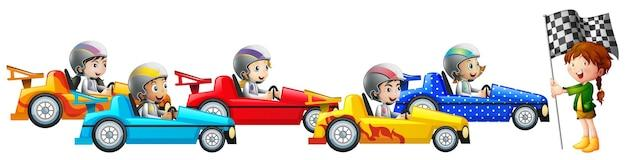
\includegraphics[width=\textwidth]{media/image1.jpg}

VOCÊ PERCEBEU COMO USAMOS OS NÚMEROS DE DIVERSAS FORMAS? ELES FORAM
ÚTEIS PARA NOS AJUDAR A CONTAR OS CARROS E A QUANTIDADE DE PARTICIPANTES
DA CORRIDA. ELES TAMBÉM NOS AJUDARAM A DEFINIR A CLASSIFICAÇÃO DOS
CORREDORES, E ATÉ NOS INDICARAM O VENCEDOR, OU SEJA, O PRIMEIRO A CRUZAR
A LINHA DE CHEGADA. ALÉM DISSO, OS NÚMEROS NÃO SERVEM SOMENTE PARA
CONTARMOS, MAS TAMBÉM PARA IDENTIFICARMOS ALGO. OS
AMIGOS CORREDORES DERAM NÚMEROS DE IDENTIFICAÇÃO A SEUS CARROS.
NOSSAS CASAS TAMBÉM TÊM NÚMEROS. ESSE É MAIS UM EXEMPLO DE
NÚMEROS IDENTIFICANDO, EM VEZ DE CONTAR.
}

\colorsec{ATIVIDADES}

\num{1} CIRCULE A FIGURA QUE CONTÉM UM NÚMERO USADO COMO CÓDIGO DE IDENTIFICAÇÃO.

%\textless{}https://stock.adobe.com/br/images/id/363300782?get\_facets=1\&order=relevance\&safe\_search=1\&k=r\%C3\%A9gua\&clickref=1100lwwNzM24\&mv=affiliate\&mv2=Freepik\&as\_camptype=\&as\_channel=affiliate\&as\_source=partnerize\&as\_campaign=Freepik\&as\_content=api\&as\_audience=srp\&sdid=6WTV6YJ5; https://stock.adobe.com/br/search?load\_type=search\&is\_recent\_search=\&search\_type=usertyped\&k=NUMERO+DE+CASA\&native\_visual\_search=\&similar\_content\_id=\&asset\_id=506848063; https://stock.adobe.com/br/search?filters\%5Bcontent\_type\%3Aphoto\%5D=1\&filters\%5Bcontent\_type\%3Aillustration\%5D=1\&filters\%5Bcontent\_type\%3Azip\_vector\%5D=1\&filters\%5Bcontent\_type\%3Avideo\%5D=1\&filters\%5Bcontent\_type\%3Atemplate\%5D=1\&filters\%5Bcontent\_type\%3A3d\%5D=1\&filters\%5Bcontent\_type\%3Aimage\%5D=1\&order=relevance\&safe\_search=1\&limit=100\&search\_page=1\&k=1+KG\&search\_type=usertyped\&acp=\&aco=1+KG\&get\_facets=0\&asset\_id=418803262. Inserir um diagrama com as 4 figuras, conforme modelo a seguir. É importante que as imagens tenham um tamanho grande, para que os alunos consigam enxergar os números.\textgreater{}

\begin{figure}[htpb!]
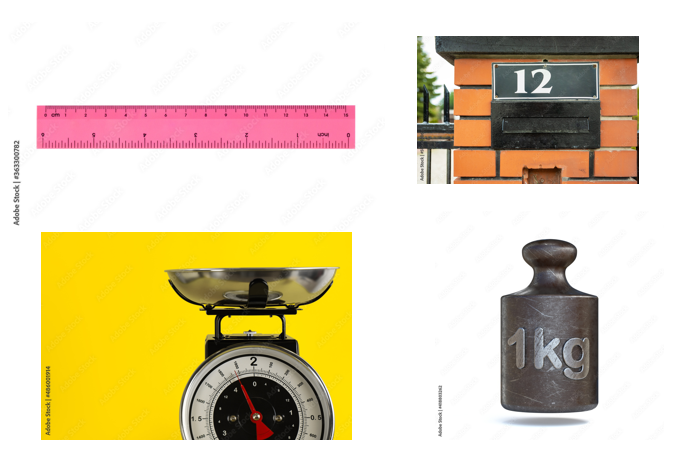
\includegraphics[width=\textwidth]{media/image2.png}
\end{figure}

\coment{Somente na figura da caixa de correio, encontramos
um número identificador. Em todas as outras imagens, os números são usados para
quantificar medidas.}

\num{2} INDIQUE OS NÚMEROS DOS CARROS NA POSIÇÃO EM QUE CRUZARAM A LINHA DE CHEGADA. CONSIDERE QUE NINGUÉM ULTRAPASSOU NINGUÉM.

%\textless{}Inserir o diagrama a seguir conforme modelo. Licenciar a figura: https://br.freepik.com/vetores-gratis/no-jogo-de-corrida-de-velocidade-o-jogador-do-driver-do-monstro-da-competicao-usou-o-carro-de-alta-velocidade-para-vencer-no-jogo\_16304604.htm\#query=carros\%20com\%20n\%C3\%BAmeros\&position=11\&from\_view=search\&track=ais.\textgreater{}

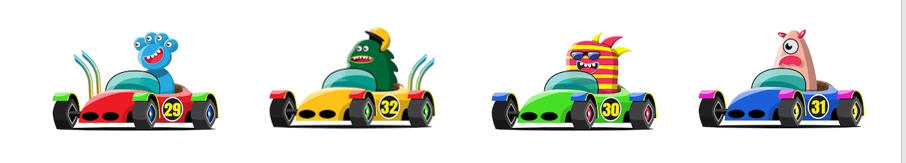
\includegraphics[width=\textwidth]{media/image3.png}

%\textless{}Criar uma figura de um podium, com círculos acima das posições, onde os alunos colocarão os números dos carros.\textgreater{}
\begin{figure}[htpb!]
\centering
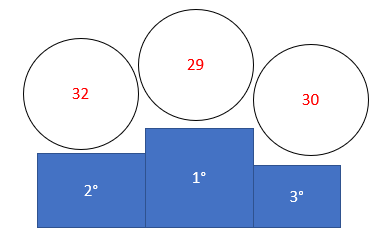
\includegraphics[width=3.92763in,height=2.54202in]{media/image4.png}
\end{figure}

\coment{Oriente os alunos acerca das funções dos números de
identificação dos carros, destacando que eles não são os números que
indicarão a ordem de chegada deles. Oriente-os para que entendam que a
ordem se inicia da esquerda para a direita.}

\num{3} LIGUE OS NÚMEROS CORRETAMENTE.

\begin{longtable}[]{@{}ll@{}}
\toprule
326 & CEM\tabularnewline
100 & CENTO E CINQUENTA E QUATRO\tabularnewline
154 & CENTO E QUARENTA\tabularnewline
451 & QUATROCENTOS E QUINZE\tabularnewline
514 & SEISCENTOS E VINTE E TRÊS\tabularnewline
140 & QUINHENTOS E CATORZE\tabularnewline
415 & TREZENTOS E VINTE E SEIS\tabularnewline
623 & QUATROCENTOS E CINQUENTA E UM\tabularnewline
\bottomrule
\end{longtable}


\num{4} ALBERTO TEM UMA COLEÇÃO DE CAMISAS DE FUTEBOL. JÚNIOR TEM UMA COLEÇÃO DE BOLAS. QUAL DAS DUAS COLEÇÕES É A MAIOR?

%\textless{}Inserir figuras: https://br.freepik.com/vetores-gratis/time-de-futebol-ou-jogadores-de-time-de-futebol-em-fundo-branco\_10600572.htm\#query=cole\%C3\%A7\%C3\%A3o\%20de\%20figurinhas\&position=11\&from\_view=search\&track=ais; https://br.freepik.com/vetores-gratis/bolas-definir-ilustracao-vetorial\_4559016.htm\#query=cole\%C3\%A7\%C3\%A3o\%20de\%20bolas\&position=0\&from\_view=search\&track=ais. Não precisa traduzir os textos em inglês, pois eles não são necessários à resolução.\textgreater{}

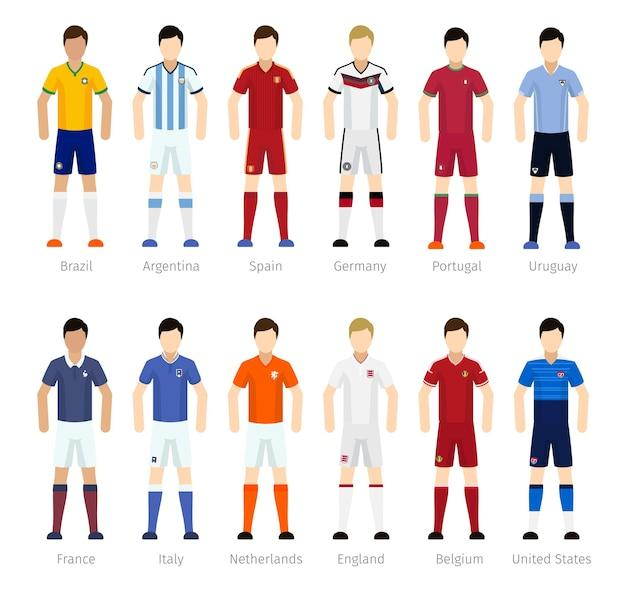
\includegraphics[width=2.90024in,height=2.77508in]{media/image5.jpg}
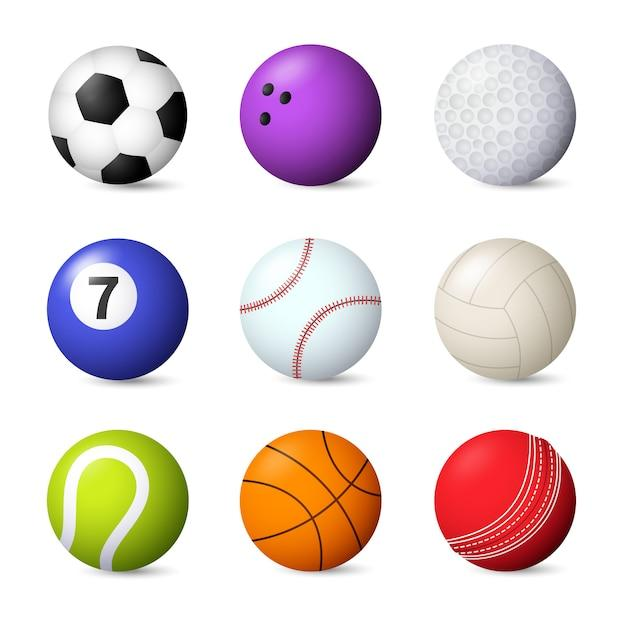
\includegraphics[width=2.59375in,height=2.59375in]{media/image6.jpg}

\coment{O aluno deve contar as duas coleções e perceber que a coleção de camisas
de Alberto é maior, pois tem mais unidades do que a coleção de Júnior.}

\num{5} AINDA SOBRE A SITUAÇÃO APRESENTADA NA ATIVIDADE ANTERIOR, RESPONDA AO QUE SE PERGUNTA A SEGUIR.

\begin{enumerate}
\item
  QUANTAS CAMISAS ALBERTO TEM? \reduline{12 camisas.\hfill}

\item
  QUANTAS BOLAS JÚNIOR TEM? \reduline{9 bolas.\hfill}

\item
  QUANTOS ITENS ALBERTO TEM EM SUA COLEÇÃO A MAIS QUE OS ITENS QUE JÚNIOR TEM EM SUA COLEÇÃO?
  \reduline{3 itens.\hfill}

\end{enumerate}

\num{6} CIRCULE O CONJUNTO DE DADOS COM O MAIOR RESULTADO.

%\textless{} Inserir um quadro com as imagens conforme o modelo a seguir. https://br.freepik.com/vetores-gratis/dados-isometricos-cubos-de-jogo-pretos-variantes-isolados-no-fundo-branco-coleta-de-todas-as-voltas-possiveis\_13090027.htm\#query=dice\&position=1\&from\_view=search\&track=sph.\textgreater{}

\begin{figure}[htpb!]
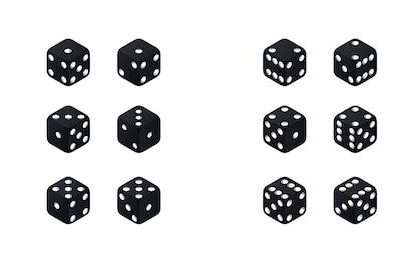
\includegraphics[width=\textwidth]{media/image7.jpg}
\end{figure}

\coment{Oriente os alunos a olharem para o resultado da face
superior do dado, da mesma forma como eles fariam ao jogar um jogo
de tabuleiro. A imagem a ser circulada é a da direita,
pois a soma dos valores dos dados representados é maior do que a soma dos valores representados nos dados da imagem da esquerda.}

\num{7} AINDA SOBRE A ATIVIDADE ANTERIOR, FAÇA O QUE SE PEDE A SEGUIR.

\begin{escolha}
\item PINTE DE AZUL O QUADRADINHO QUE TEM O NÚMERO DA SOMA DOS DADOS DA DIREITA.

\item PINTE DE VERDE O QUADRADINHO QUE TEM O NÚMERO DA SOMA DOS DADOS DA ESQUERDA.

\item PINTE DE AMARELO A DIFERENÇA ENTRE AS DUAS SOMAS.
\end{escolha}

\begin{longtable}[]{@{}lllll@{}}
\toprule
12 & 24 & 30 & 40 & 10\tabularnewline
6 & 21 & 20 & 8 & 5\tabularnewline
7 & 18 & 4 & 22 & 13\tabularnewline
19 & 2 & 1 & 23 & 15\tabularnewline
25 & 11 & 9 & 17 & 32\tabularnewline
\bottomrule
\end{longtable}

\coment{O aluno deve pintar o número 18 de verde, o número 22 de azul e o número
4 de amarelo.}

\num{8} ESCREVA OS SEGUINTES NÚMEROS EM ORDEM CRESCENTE.

\begin{escolha}
\item 516 -- 645 -- 215 -- 326 - 789

\reduline{215 -- 326 -- 516 -- 645 -- 789\hfill}


\item 132 -- 165 -- 112 -- 115 -- 100

\reduline{100 -- 112 -- 115 -- 132 -- 165\hfill}


\item 325 -- 854 -- 127 -- 974 -- 546

\reduline{127 -- 325 -- 546 -- 854 -- 974\hfill}


\item 415 -- 418 -- 411 -- 410 -- 417

\reduline{410 -- 411 -- 415 -- 417 -- 418\hfill}


\item 798 -- 987 -- 879 -- 897 -- 978

\reduline{798 -- 879 -- 897 -- 978 -- 987\hfill}


\item 623 -- 236 -- 362 -- 326 -- 263

\reduline{236 -- 263 -- 326 -- 362 -- 623\hfill}
\end{escolha}

\num{9} ESCREVA OS SEGUINTES NÚMEROS EM ORDEM DECRESCENTE.

\begin{escolha}
\item 564 -- 456 -- 546 -- 645 -- 465

\reduline{645 -- 564 -- 546 -- 465 -- 456\hfill}

\item 138 -- 831 -- 318 -- 183 -- 813

\reduline{831 -- 813 -- 318 -- 183 -- 138\hfill}

\item 715 -- 517 -- 751 -- 571 -- 175

\reduline{751 -- 715 -- 571 -- 517 -- 175\hfill}

\item 833 -- 383 -- 838 -- 338 -- 388

\reduline{838 -- 833 -- 388 -- 383 -- 338\hfill}

\item 717 -- 177 -171 -- 117 -- 771

\reduline{771 -- 717 -- 177 -- 171 -- 117\hfill}

\item 100 -- 200 -- 300 - 400 -- 500

\reduline{500 -- 400 -- 300 -- 200 -- 100\hfill}
\end{escolha}

\num{10} JERÔNIMO MORA NA CASA 328 DA RUA SANTOS, EM SUA
CIDADE. LIGUE CORRETAMENTE OS ALGARISMOS DO NÚMERO DA CASA ÀS ORDENS
CORRESPONDENTES.

\begin{longtable}[]{@{}ll@{}}
\toprule
3 & DEZENAS\tabularnewline
2 & CENTENAS\tabularnewline
8 & UNIDADES\tabularnewline
\bottomrule
\end{longtable}

\num{11} PINTE OS QUADRADOS COM A COR DA ORDEM CORRESPONDENTE.

%\textless{}Criar um afigura conforme o modelo a seguir.\textgreater{}

\begin{figure}[htpb!]
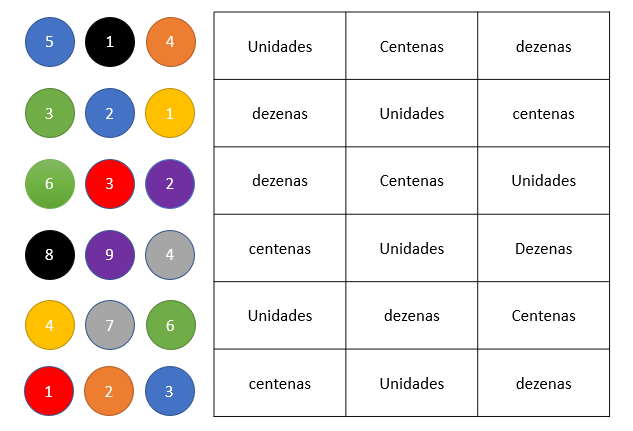
\includegraphics[width=5.90556in,height=4.02083in]{media/image8.png}
\end{figure}

\rosa{
\begin{longtable}[]{@{}lll@{}}
\toprule
laranja & azul & Preto\tabularnewline
azul & amarelo & Verde\tabularnewline
vermelho & verde & Roxo\tabularnewline
preto & cinza & Roxo\tabularnewline
verde & cinza & Amarelo\tabularnewline
vermelho & azul & Laranja\tabularnewline
\bottomrule
\end{longtable}
}

\num{12} OS TRÊS COMPETIDORES REPRESENTADOS ESTÃO NO PÓDIO. ELES TÊM OS NOMES ESCRITOS NA CAMISETA. DESCUBRA QUAL É A PONTUAÇÃO DE CADA UM DELES E ESCREVA SEUS NOMES NA TABELA.

%\textless{}Inserir a figura de referência: https://br.freepik.com/vetores-gratis/podio-esportes\_1040693.htm\#query=podium\%20com\%20competidores\&position=1\&from\_view=search\&track=ais. Acrescente os nomes dos competidores, conforme o modelo a seguir.\textgreater{}

\begin{figure}[htpb!]
\centering
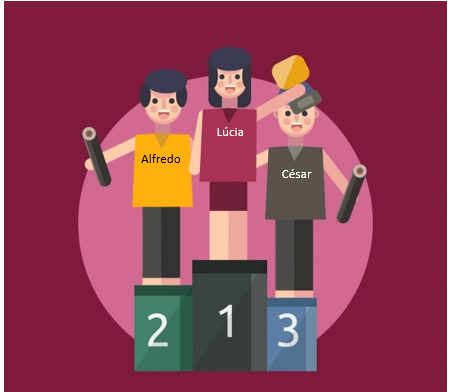
\includegraphics[width=3.84950in,height=3.34590in]{media/image9.png}
\end{figure}

\begin{longtable}[]{@{}ll@{}}
\toprule
\textbf{PONTOS} & \textbf{NOMES}\tabularnewline
1~000 PONTOS & \rosa{César}\tabularnewline
1~005 PONTOS & \rosa{Lúcia}\tabularnewline
1~0004 PONTOS & \rosa{Alfredo}\tabularnewline
\bottomrule
\end{longtable}

\coment{É importante que os alunos compreendam que o primeiro
colocado deve ter feito a maior quantidade de pontos, e assim por
diante.}

\pagebreak
\num{13} A RETA NUMERADA A SEGUIR REPRESENTA UMA RUA QUALQUER DE UM BAIRRO. LIGUE AS CASAS ÀS SUAS RESPECTIVAS POSIÇÕES CONFORME O NÚMERO.

%\textless{}Criar uma reta numérica conforme o modelo a seguir. Depois colocar a figura de referência: https://br.freepik.com/vetores-gratis/pacote-de-belas-fachadas-de-casas-desenhadas-a-mao\_1198631.htm\#page=2\&query=casas\%20coloridas\&position=11\&from\_view=search\&track=ais com os respectivos números conforme o modelo.

\begin{figure}[htpb!]
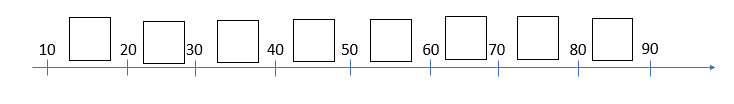
\includegraphics[width=\textwidth]{media/image10.png}

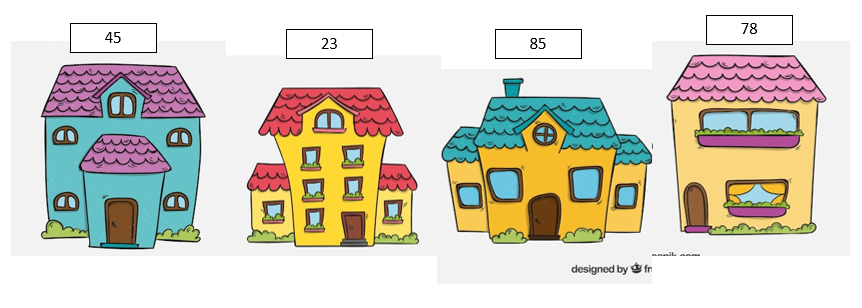
\includegraphics[width=\textwidth]{media/image11.png}
\end{figure}

\num{14} ESCREVA OS NÚMEROS A SEGUIR COM ALGARISMOS.

\begin{longtable}[]{@{}ll@{}}
\toprule
SEISCENTOS E DEZENOVE & \rosa{619}\tabularnewline
OITOCENTOS E TRINTA E SETE & \rosa{837}\tabularnewline
NOVECENTOS E QUARENTA E UM & \rosa{941}\tabularnewline
CENTO E DOIS & \rosa{102}\tabularnewline
CENTO E TRINTA E OITO & \rosa{138}\tabularnewline
DUZENTOS E VINTE E CINCO & \rosa{225}\tabularnewline
TREZENTOS E OITENTA E QUATRO & \rosa{384}\tabularnewline
QUATROCENTOS E QUINZE & \rosa{415}\tabularnewline
QUINHENTOS E SETENTA E SETE & \rosa{577}\tabularnewline
SETECENTOS E DEZESSEIS & \rosa{716}\tabularnewline
CENTO E CINQUENTA E TRÊS & \rosa{153}\tabularnewline
\bottomrule
\end{longtable}

\colorsec{TREINO}

\num{1} NA CARTEIRINHA DA ESCOLA DE JÚLIA, APARECE SUA FOTO, SEU NOME E O NÚMERO DO
REGISTRO DE MATRÍCULA. NO CASO DE JÚLIA, ESSE NÚMERO É O 363. ESSE NÚMERO INDICA

\begin{escolha}
\item
  QUANTIDADE.
\item
  ORDEM.
\item
  MEDIDA.
\item
  IDENTIFICAÇÃO.
\end{escolha}

\coment{SAEB: Reconhecer o que os números naturais indicam em diferentes
situações: quantidade, ordem, medida ou código de identificação.
BNCC: EF01MA01 -- Utilizar números naturais como indicador de quantidade
ou de ordem em diferentes situações cotidianas e reconhecer situações em
que os números não indicam contagem nem ordem, mas sim código de
identificação.}


\num{2} NA IMAGEM, MOSTRAM-SE QUATRO COLEÇÕES DE AMIGOS QUE GOSTAM DE COLECIONAR
BOLINHAS DE GUDE.

%\textless{}Criar a figura conforme modelo a seguir.\textgreater{}

\begin{figure}[htpb!]
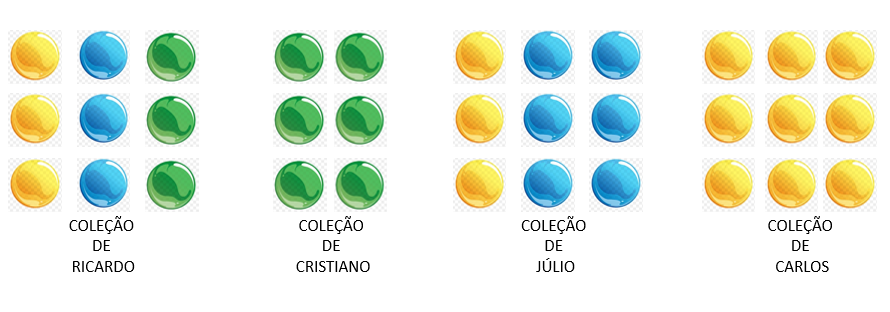
\includegraphics[width=\textwidth]{media/image12.png}
\end{figure}

QUAL COLEÇÃO TEM A MAIOR QUANTIDADE DE BOLAS DE UMA ÚNICA COR?

\begin{escolha}
\item
  CARLOS.
\item
  CRISTIANO.
\item
  JÚLIO.
\item
  RICARDO.
\end{escolha}

\coment{SAEB: Comparar ou ordenar quantidade de objetos (até 2 ordens).

BNCC: EF01MA05 -- Comparar números naturais de até duas ordens em
situações cotidianas, com e sem suporte da reta numérica.}

\num{3} ENTRE 0 E 100, QUANTOS NÚMEROS TERMINAM COM O NÚMERO ZERO NA ORDEM DAS UNIDADES?

\begin{escolha}
\item
  1.
\item
  9.
\item
  10.
\item
  11.
\end{escolha}

\coment{SAEB: Identificar a ordem ocupada por um algarismo OU seu valor
posicional (ou valor relativo) em um número natural de até 3 ordens.

BNCC: EF01MA03 -- Estimar e comparar quantidades de objetos de dois
conjuntos (em torno de 20 elementos), por estimativa e/ou por
correspondência (um a um, dois a dois) para indicar ``tem mais'', ``tem
menos'' ou ``tem a mesma quantidade''.}

\chapter{JUNTAR OU TIRAR?}
\markboth{Módulo 2}{}

\coment{Neste módulo, vamos desenvolver a habilidade de desenvolvimento de
cálculos, tanto no sentido de escolher a melhor estratégia, quanto no
sentido de resolver o problema. Faremos essa abordagem de forma
abstrata, mas também de forma contextualizada, com o fim de desenvolver
nos alunos a motivação para resolverem problemas reais.\\
HABILIDADES DA BNCC: EF01MA07, EF01MA08.}


\colorsec{HABILIDADES DO SAEB}

\begin{itemize}
\item Calcular o resultado de adições e subtrações, envolvendo número
naturais de até 3 ordens.

\item Compor ou decompor números naturais de até 3 ordens por meio de
diferentes adições.

\item Resolver problemas de adição ou de subtração, envolvendo números
naturais de até 3 ordens, com os significados de juntar, acrescentar,
separar ou retirar.
\end{itemize}

\conteudo{
MÁRCIA GANHOU DO PAI DUAS NOTAS DE DEZ REAIS E DECIDIU QUE
QUERIA COMPRAR UM BRINQUEDO QUE CUSTAVA QUINZE REAIS. MÁRCIA PERCEBEU
QUE TINHA UM PROBLEMA: PARA SABER SE ELA TERIA CONDIÇÕES DE COMPRAR
AQUELE BRINQUEDO, ELA TERIA DE DESCOBRIR QUANTO DINHEIRO TINHA, MAS SEU PAI
RESOLVEU AJUDAR. ELE PEGOU A QUANTIDADE DE PALITOS EQUIVALENTE AO VALOR DAS
NOTAS. OBSERVE:

%\textless{}Criar uma ilustração com duas carreiras de 10 palitos alinhadas a uma cédula de 10 reais, conforme o modelo a seguir. https://www.istockphoto.com/br/foto/dez-real-brasileiro-gm181402095-26926813?utm\_campaign=srp\_photos\_inline\&utm\_content=https\%3A\%2F\%2Fwww.pexels.com\%2Fprocurar\%2F10\%2520reais\%2F\&utm\_medium=affiliate\&utm\_source=pexels\&utm\_term=10+reais https://br.freepik.com/fotos-premium/uma-partida-com-cabeca-verde-em-um-fundo-branco\_31512045.htm\#page=3\&query=palito\%20de\%20f\%C3\%B3sforo\&position=18\&from\_view=search\&track=ais\textgreater{}

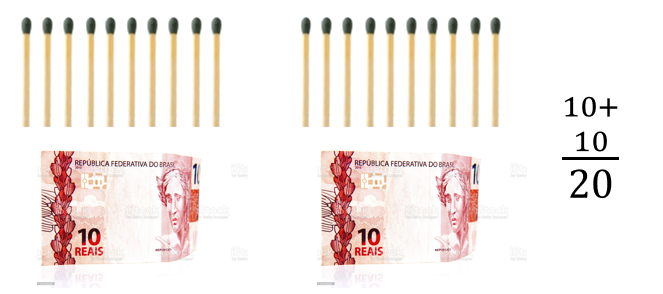
\includegraphics[width=\textwidth]{media/image13.png}

MÁRCIA CONTOU OS PALITOS E PERCEBEU QUE TINHA 20 REAIS. AGORA, ELA
PRECISAVA SABER SE ESSES 20 REAIS SERIAM SUFICIENTES PARA COMPRAR O
BRINQUEDO. A PRÓPRIA MÁRCIA PEGOU MAIS QUINZE PALITINHOS E OS ALINHOU DA
SEGUINTE FORMA:

%\textless{}Criar uma figura com duas linhas de palito alinhados. Na primeira linha 20 e na segunda linha 15. Colocar a operação ao lado, conforme modelo a seguir.\textgreater{}

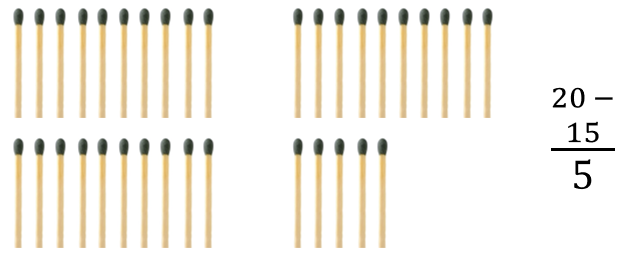
\includegraphics[width=\textwidth]{media/image14.png}

MÁRCIA FICOU MUITO FELIZ AO PERCEBER QUE PODERIA COMPRAR SEU BRINQUEDO.
E AINDA LHE SOBRARIAM CINCO REAIS PARA COMPRAR UM LANCHE.
}

\pagebreak
\colorsec{ATIVIDADES}

\num{1} PINTE O FOGUETE COM AS CORES CORRETAS. DESCUBRA AS CORES RESOLVENDO AS
ADIÇÕES.

%\textless{}Inserir um quadro conforme o modelo a seguir. https://br.freepik.com/vetores-premium/foguete-de-desenho-bonito-de-cor-planilha-para criancas\_22159996.htm\#page=6\&query=para\%20colorir\%20foguete\&position=7\&from\_view=search\&track=ais.\textgreater{}

\begin{figure}[htpb!]
\centering
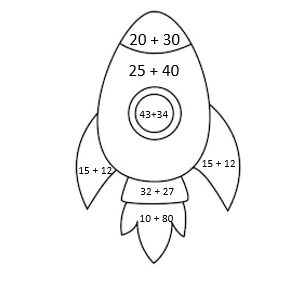
\includegraphics[width=3.09611in,height=2.97268in]{media/image15.png}
\end{figure}

\begin{mdframed}[linewidth=2pt,linecolor=salmao,roundcorner=10pt]\Huge
\textcolor{green}{59}\hfill\textcolor{purple}{65}\hfill\textcolor{blue}{77}\hfill\textcolor{orange}{90}\hfill\textcolor{red}{50}\hfill\textcolor{yellow}{27}
\end{mdframed}


\coment{Oriente os alunos a resolverem as adições primeiro, antes
de começarem a pintar o foguete. No quadro à esquerda, temos as
resoluções das adições. Nele, o aluno deve pintar o pedaço do foguete com
a cor correspondente.}

%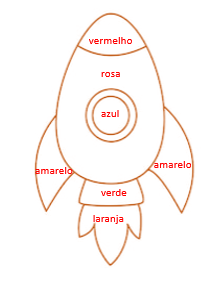
\includegraphics[width=1.43098in,height=1.89472in]{media/image16.png}

\num{2} EFETUE AS ADIÇÕES A SEGUIR.

\begin{center}
\begin{tabular}{llllllllllllll}
51 &  &  & 32 &  &  & 13 &  &  & 74 &  &  & 23 &  \\
12 & $+$ &  & 21 & $+$ &  & 15 & $+$ &  & 20 & $+$ &  & 31 & $+$ \\ \cline{1-1} \cline{4-4} \cline{7-7} \cline{10-10} \cline{13-13}
\rosa{63} &  &  & \rosa{53} &  &  & \rosa{28} &  &  & \rosa{94} &  &  & \rosa{54} & 
\end{tabular}
\end{center}

\begin{center}
\begin{tabular}{llllllllllllll}
24 &  &  & 41 &  &  & 11 &  &  & 10 &  &  & 29 &  \\
13 & $+$ &  & 36 & $+$ &  & 11 & $+$ &  & 60 & $+$ &  & 15 & $+$ \\ \cline{1-1} \cline{4-4} \cline{7-7} \cline{10-10} \cline{13-13}
\rosa{37} &  &  & \rosa{77} &  &  & \rosa{22} &  &  & \rosa{70} &  &  & \rosa{44} & 
\end{tabular}
\end{center}

\coment{Oriente os alunos a iniciarem as adições pela ordem das
unidades, seguindo pela ordem das dezenas e, finalmente, passando à das centenas,
para obter o resultado.}

\num{3} EFETUE AS SUBTRAÇÕES A SEGUIR.

\begin{center}
\begin{tabular}{llllllllllllll}
51 &  &  & 32 &  &  & 15 &  &  & 74 &  &  & 31 &  \\
12 & $-$ &  & 21 & $-$ &  & 13 & $-$ &  & 20 & $-$ &  & 23 & $-$ \\ \cline{1-1} \cline{4-4} \cline{7-7} \cline{10-10} \cline{13-13}
\rosa{39} &  &  & \rosa{11} &  &  & \rosa{2} &  &  & \rosa{54} &  &  & \rosa{8} & 
\end{tabular}
\end{center}

\begin{center}
\begin{tabular}{llllllllllllll}
24 &  &  & 41 &  &  & 11 &  &  & 60 &  &  & 29 &  \\
13 & $-$ &  & 36 & $-$ &  & 11 & $-$ &  & 10 & $-$ &  & 15 & $-$ \\ \cline{1-1} \cline{4-4} \cline{7-7} \cline{10-10} \cline{13-13}
\rosa{11} &  &  & \rosa{5} &  &  & \rosa{0} &  &  & \rosa{50} &  &  & \rosa{14} & 
\end{tabular}
\end{center}

\coment{Alguns termos desta atividade são iguais aos
termos da atividade anterior. É importante que você destaque isso com os
alunos, com o fim de que eles percebam que os resultados são diferentes,
em função da operação. É importante que percebam com clareza que os
resultados obtidos nas subtrações são sempre menores do que os
resultados obtidos nas adições quando os números envolvidos são os mesmos.}

\num{4} PARA CONSEGUIR DAR O PRÓXIMO PASSO, O PATO PRECISA DESCOBRIR O PRÓXIMO VALOR. AJUDE-O.

%\textless{}Criar um caminho conforme o modelo a seguir. As referências dos patos são: https://br.freepik.com/vetores-premium/desenho-de-pato-bonitinho-posando\_22341752.htm\#query=pato\&position=35\&from\_view=search\&track=sph

%https://br.freepik.com/vetores-gratis/pato-fofo-em-branco\_7042481.htm\#query=pato\&position=0\&from\_view=search\&track=sph

\begin{figure}[htpb!]
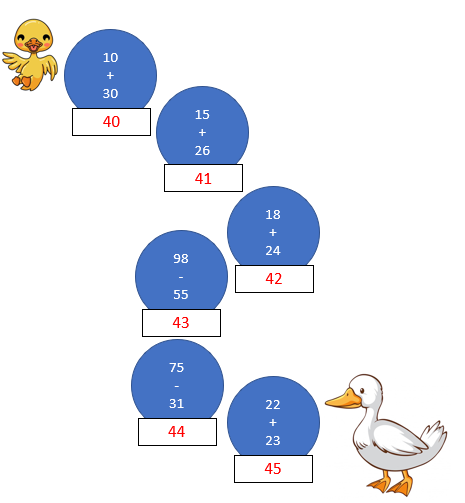
\includegraphics[width=4.84443in,height=5.24031in]{media/image17.png}
\end{figure}

\num{5} PAULO TEM UMA COLEÇÃO ENORME DE FIGURINHAS: 20 FIGURINHAS DE
JOGADORES DE FUTEBOL, 15 FIGURINHAS DE CARROS ESPORTIVOS, 17 FIGURINHAS
DE JOGOS DE \textit{VIDEOGAME} E 26 FIGURINHAS DE SEU PERSONAGEM
PREFERIDO. NA ESCOLA, PAULO PERDEU 10 FIGURINHAS, JOGANDO TAPÃO. COM
QUANTAS FIGURINHAS ELE FICOU NO TOTAL?

\reduline{O aluno precisa
usar a adição e a subtração para obter a resposta. Oriente as crianças caso
estejam com dificuldade de encontrar a resposta correta, além de ler o
problema com eles, visto que ainda têm dificuldade de leitura e escrita.
Se necessário, distribua palitos para auxiliar os alunos na contagem.
Oriente-os a fazer uma adição por vez, assim como a fazer a subtração
somente no final. (15 + 17 + 26 = 58) (\rightarrow \ \ 58 - 10 = 48).\hfill}

\num{6} JOANA TEM MUITA VONTADE DE COMPARAR UMA BOLA NOVA, DEPOIS QUE PERDEU A QUE TINHA, E DESCOBRIU QUE, NA LOJA PERTO DE SUA CASA, UMA BEM LEGAL CUSTA 56 REAIS. A MENINA ABRIU SEU COFRINHO E CONTOU 25 REAIS, MAS JÁ CONTAVA COM A MESADA DE 15 REAIS QUE RECEBERIA NO FINAL DA SEMANA. QUANTO AINDA VAI FALTAR PARA JOANA COMPRAR A BOLA?

\linhas{4}


\num{7} DEMONSTRE VÁRIAS FORMAS DE FORMARMOS O NUMERO 100 POR MEIO DA ADIÇÃO DE
DUAS PARCELAS.

\begin{center}
\begin{tabular}{llllllllllllll}
50 &  &  & \mbox{} &  &  & \mbox{} &  &  & \mbox{} &  &  & \mbox{} &  \\
50 & $+$ &  & \mbox{} & $+$ &  & \mbox{} & $+$ &  & \mbox{} & $+$ &  & \mbox{} & $+$ \\ \cline{1-1} \cline{4-4} \cline{7-7} \cline{10-10} \cline{13-13}
100 &  &  & 100 &  &  & 100 &  &  & 100 &  &  & 100 & 
\end{tabular}
\end{center}

\begin{center}
\begin{tabular}{llllllllllllll}
\mbox{} &  &  & \mbox{} &  &  & \mbox{} &  &  & \mbox{} &  &  & \mbox{} &  \\
\mbox{} & $+$ &  & \mbox{} & $+$ &  & \mbox{} & $+$ &  & \mbox{} & $+$ &  & \mbox{} & $+$ \\ \cline{1-1} \cline{4-4} \cline{7-7} \cline{10-10} \cline{13-13}
100 &  &  & 100 &  &  & 100 &  &  & 100 &  &  & 100 & 
\end{tabular}
\end{center}

\coment{Crie alguns
exemplos com os alunos e oriente-os a utilizarem números mais simples,
como 10, 20 etc. Aproveite para lembrar-lhes o conceito de parcelas,
pois, talvez, alguns não saibam ainda o que significa essa palavra.
A atividade pode ser aproveitada para ampliar o vocabulário dos alunos.}

\num{8} DEMONSTRE VÁRIAS FORMAS DE FORMARMOS O NUMERO 10 POR MEIO DA SUBTRAÇÃO DE
DUAS PARCELAS.

\begin{center}
\begin{tabular}{llllllllllllll}
100 &  &  & \mbox{} &  &  & \mbox{} &  &  & \mbox{} &  &  & \mbox{} &  \\
90 & $-$ &  & \mbox{} & $-$ &  & \mbox{} & $-$ &  & \mbox{} & $-$ &  & \mbox{} & $-$ \\ \cline{1-1} \cline{4-4} \cline{7-7} \cline{10-10} \cline{13-13}
10 &  &  & 10 &  &  & 10 &  &  & 10 &  &  & 10 & 
\end{tabular}
\end{center}

\begin{center}
\begin{tabular}{llllllllllllll}
\mbox{} &  &  & \mbox{} &  &  & \mbox{} &  &  & \mbox{} &  &  & \mbox{} &  \\
\mbox{} & $-$ &  & \mbox{} & $-$ &  & \mbox{} & $-$ &  & \mbox{} & $-$ &  & \mbox{} & $-$ \\ \cline{1-1} \cline{4-4} \cline{7-7} \cline{10-10} \cline{13-13}
10 &  &  & 10 &  &  & 10 &  &  & 10 &  &  & 10 & 
\end{tabular}
\end{center}


\num{9} RESOLVA O ENIGMA E DESCUBRA QUAL É O NÚMERO. PINTE-O NO QUADRO.

\begin{itemize}
\item Sou maior que 5.

\item sou menor que 50.

\item uma das minhas parcelas pode ser 12.

\item uma das minhas parcelas também pode ser 10.

\item se uma das minhas parcelas for 20, a outra não pode ser maior do que dois.
\end{itemize}

\begin{center}
{\LARGE
\begin{tabular}{|c|c|c|}
\hline
22 & 12 & 10 \\ \hline
32 & 50 & 5 \\ \hline
20 & 2 & 42 \\ \hline
\end{tabular}
}
\end{center}

\coment{O número em questão é o 22.}

\num{10} PINTE DA MESMA COR OS NÚMEROS QUE, ADICIONADOS, EM TRÊS PARCELAS, PODEM
FORMAR OS NÚMEROS QUE SE PEDEM.

\begin{center}
{\LARGE
\begin{tabular}{|c|c|c|c|}
\hline
2 & 10 & 5 & \textcolor{yellow}{10} \\ \hline
25 & 3 & 22 & \textcolor{green}{50} \\ \hline
28 & 50 & 15 & \textcolor{blue}{100} \\ \hline
\end{tabular}
}
\end{center}

\coment{Explique aos alunos que só existe uma combinação possível
para cada número. Oriente também a pintarem as parcelas na cor
equivalente aos resultados esperados na coluna do lado direito. Peça
a eles que confiram antes de pintar. As combinações são:

\begin{longtable}[]{@{}lllll@{}}
\toprule
amarelo & verde & amarelo & & \(2 + 3 + 5 = 10\)\tabularnewline
verde & amarelo & azul & & \(25 + 10 + 15 = 50\)\tabularnewline
azul & azul & verde & & \(28 + 50 + 22 = 100\)\tabularnewline
\bottomrule
\end{longtable}
}

\num{11} PATRICK QUER VENDER SEU ÁLBUM DE FIGURINHAS POR 56 REAIS. UM AMIGUINHO
QUER COMPRÁ-LO, MAS SÓ TEM 13 REAIS. ALÉM DISSO, SÓ PODERA PAGAR O RESTO
EM DUAS VEZES, E A PRIMEIRA PARCELA DEVERIA SER MENOR QUE A PRIMEIRA.
ELABORE TRÊS FORMAS DE PAGAMENTO PARA O AMIGO DE PATRICK.

\begin{longtable}[]{@{}lll@{}}
\toprule
& 56 -- 13 = & \rosa{43}\tabularnewline
& &\tabularnewline
& MENOR & MAIOR\tabularnewline
1° FORMATO & \rosa{20} & \rosa{23}\tabularnewline
& MENOR & MAIOR\tabularnewline
2° FORMATO & &\tabularnewline
& MENOR & MAIOR\tabularnewline
3° FORMATO & &\tabularnewline
\bottomrule
\end{longtable}

\coment{Oriente os
alunos a primeiro descobrirem quanto falta para o amigo de Patrick pagar
pelo álbum de figurinhas.}

\num{12} ASSINALE UMA FORMA DE AGRUPARMOS 45 REAIS UTILIZANDO AS SEGUINTES
CÉDULAS.

%\textless{}Criar uma figura conforme o modelo a seguir. Se necessário desconfigure as notas de reais, contanto que as cédulas fictícias tenham o mesmo valor. Coloque uma bola para que o aluno assinale. 

\begin{figure}[htpb!]
\centering
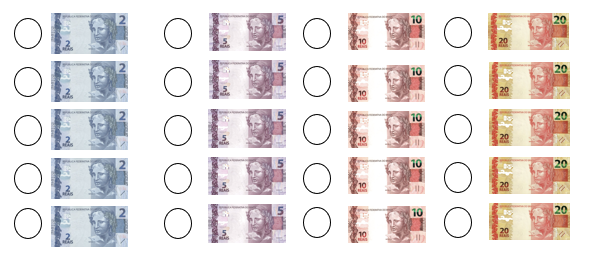
\includegraphics[width=5.90556in,height=2.71667in]{media/image18.png}
\end{figure}

\coment{Há várias respostas possíveis. É
importante que o aluno consiga compreender a ideia de composição por
diferentes adições. Peça às crianças que criem outra forma além da
encontrada na atividade e registrem na lousa. Esta atividade é
importante para trabalhar educação financeira. Algumas das combinações
podem ser: (20 + 20 + 5,\ \ \ \ 10 + 10 + 10 + 10 + 5), 2 + 2 + 2 + 2 + 2 + 10 + 20 + 5 etc.}

\num{13} NUMA PARTIDA DE FUTEBOL, ESTAVAM JOGANDO DOIS TIMES: O TIME A E O TIME B. FORAM MARCADOS 10 GOLS, E O TIME A VENCEU A PARTIDA. IDENTIDIQUE OS POSSÍVEIS PLACARES.

%\textless{}Inserir uma figura conforme o modelo a seguir. https://br.freepik.com/vetores-gratis/conjunto-de-simbolos-ou-emblemas-de-escudo-de-nove\_8998384.htm\#query=escudo\%20de\%20time\&position=5\&from\_view=search\&track=ais.\textgreater{}

\begin{figure}[htpb!]
\centering
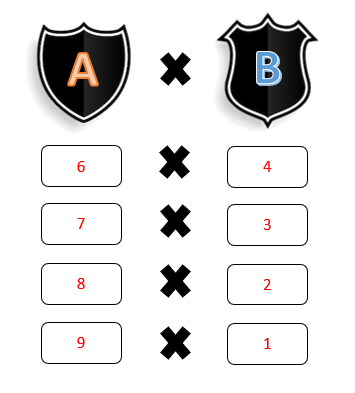
\includegraphics[width=2.78474in,height=3.08282in]{media/image19.png}
\end{figure}

\coment{Oriente os alunos sobre o fato de haver exatamente quatro
resultados possíveis.}

\num{14} A MÃE DE REINALDO VAI CHAMAR 50 PESSOAS PARA A FESTA DE ANIVERSÁRIO DELE,
MAS REINALDO TEM 10 TIOS, 8 TIAS, 15 PRIMOS, 9 AMIGOS E 4 VIZINHOS. SOBRE ESSA SITUAÇÃO, RESPONDA AO QUE SE PERGUNTA A SEGUIR.

\begin{escolha}
\item CONVIDANDO-SE TODAS ESSAS PESSOAS MENCIONADAS, PODEM-SE ACRESCENTAR CONVIDADOS OU SERÁ NECESSÁRIO RETIRAR PESSOAS DA LISTA?

\reduline{O aluno precisa somar o número de pessoas: (10 + 8 + 15 + 9 + 4 = 46). Com isso, ele descobre que se podem acrescentar quatro pessoas ainda.\hfill}

\item QUANTOS CONVIDADOS PODEM SER ACRESCENTADOS OU QUANTAS PESSOAS PRECISAM SER
  RETIRADAS?

\reduline{Subtraindo-se o número de pessoas da lista do número de convites para a festa, tem-se: (50 - 46 = 4). Podem ser convidadas ainda outras quatro pessoas.\hfill}
\end{escolha}

\num{15} ANALISE AS CAIXAS COM AS FIGURAS GEOMÉTRICAS. PRECISAMOS ORGANIZÁ-LAS PARA QUE CADA CAIXA TENHA A MESMA QUANTIDADE DE FIGURAS. SÃO 16 CÍRCULOS, 16 QUADRADOS E 16 TRIÂNGULOS; ENTÃO CADA CAIXA DEVE CONTER 4 QUADRADOS, 4 TRIÂNGULOS E 4 CÍRCULOS.

%\textless{}Inserir uma figura com quatro caixas, identificadas por letras, contendo círculos, quadrados e triângulos, espalhados de forma aleatória, conforme o modelo a seguir.

\begin{figure}[htpb!]
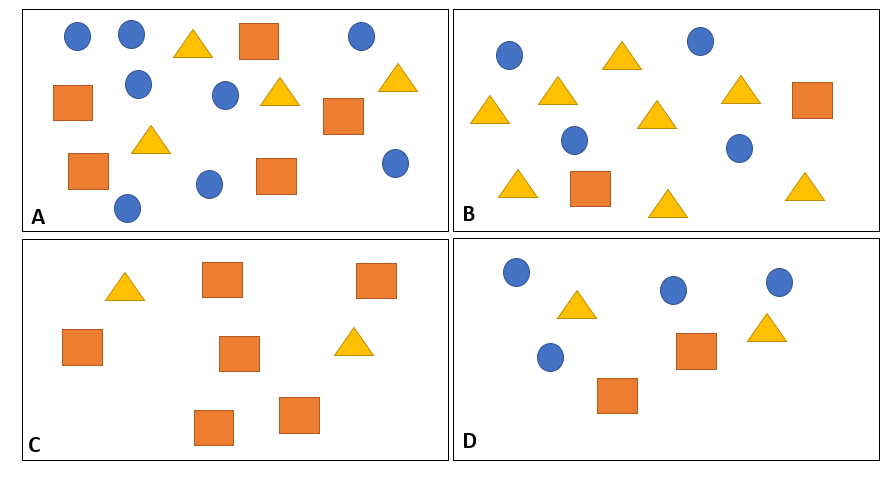
\includegraphics[width=5.90556in,height=3.22917in]{media/image20.png}
\end{figure}

\begin{escolha}
\item QUANTOS CÍRCULOS DEVEM SER RETIRADOS DA CAIXA \textbf{A}?

\reduline{2  círculos.\hfill}

\item QUANTOS TRIÂNGULOS DEVEM SER RETIRADOS DA CAIXA \textbf{B}?

\reduline{4 triângulos.\hfill}

\item QUANTOS TRIÂNGULOS DEVEM SER ADICIONADOS ÀS CAIXAS \textbf{C} E \textbf{D}?

\reduline{2 triângulos a cada uma.\hfill}

\item QUANTOS QUADRADOS DEVEM SER RETIRADOS DA CAIXA \textbf{A}?

\reduline{1 quadrado.\hfill}

\item QUANTOS QUADRADOS DEVEM SER RETIRADOS DA CAIXA \textbf{C}?

\reduline{2 quadrados.\hfill}

\item QUANTOS QUADRADOS DEVEM SER ADICIONADOS ÀS CAIXAS \textbf{B} E \textbf{D}?

\reduline{2 quadrados a cada uma.\hfill}

\item CRIANDO-SE UMA QUINTA CAIXA (\textbf{E}), COM TODAS AS FIGURAS JUNTAS, ESSA CAIXA \textbf{E} FICARIA COM QUANTAS FIGURAS?

\reduline{(16 + 16 + 16 + 16 = 64) figuras.\hfill}
\end{escolha}

\colorsec{TREINO}

\num{1} BENÍCIO E BERNARDO SÃO IRMÃOS E RESOLVERAM JUNTAR TODAS AS
SUAS FIGURINHAS: AS 25 DE BENÍCIO E AS 32 DE BERNARDO. QUANTAS FIGURINHAS OS
IRMÃOS TÊM JUNTOS?

\begin{escolha}
\item
  7.
\item
  25.
\item
  32.
\item
  57.
\end{escolha}

\coment{SAEB: Calcular o resultado de adições e subtrações, envolvendo
número naturais de até 3 ordens.
BNCC: EF01MA08 -- Resolver e elaborar problemas de adição e de subtração,
envolvendo números de até dois algarismos, com os significados de juntar, acrescentar, separar e retirar, com o suporte de imagens e/ou material manipulável, utilizando estratégias e formas de registro pessoais.}

\num{2} EM UM COLÉGIO, O PRIMEIRO ANO DIVIDIU-SE EM DOIS TIMES PARA JOGAREM BASQUETE: O TIME PEQUENOS CAMPEÕES E O TIME BASQUETEIROS. AO TODO, NO JOGO, OS DOIS TIMES FIZERAM 30 CESTAS, E OS PEQUENOS CAMPEÕES VENCERAM OS BASQUETEIROS. ENTRE AS OPÇÕES A SEGUIR, QUAL FOI O PLACAR FINAL DA PARTIDA?

\begin{escolha}
\item
  PEQUENOS CAMPEÕES 16 X BASQUETEIROS 15.
\item
  PEQUENOS CAMPEÕES 16 X BASQUETEIROS 14.
\item
  PEQUENOS CAMPEÕES 15 X BASQUETEIROS 14.
\item
  PEQUENOS CAMPEÕES 15 X BASQUETEIROS 13.
\end{escolha}

\coment{SAEB: Compor ou decompor números naturais de até 3 ordens por
meio de diferentes adições.
BNCC: EF01MA07 -- Compor e decompor número de até duas ordens, por meio
de diferentes adições, com o suporte de material manipulável,
contribuindo para a compreensão de características do sistema de
numeração decimal e o desenvolvimento de estratégias de cálculo.}


\num{3} VINÍCIUS QUER COMPRAR UM LANCHE, MAS SÓ TEM 15 REAIS. PEDIU A SUA MÃE, E
ELA LHE DEU MAIS 12 REAIS. DEPOIS, PEDIU DINHEIRO À AVÓ, E ELA
LHE DEU MAIS 10 REAIS. ENTÃO, VINÍCIUS PERCEBEU QUE CONSEGUIRIA COMPRAR O LANCHE E UM SORVETE DE 5 REAIS. QUAL É O PREÇO DO LANCHE?

\begin{escolha}
\item
  15.
\item
  32.
\item
  37.
\item
  42.
\end{escolha}

\coment{SAEB: Resolver problemas de adição ou de subtração, envolvendo
números naturais de até 3 ordens, com os significados de juntar,
acrescentar, separar ou retirar.
BNCC: EF01MA08 -- Resolver e elaborar problemas de adição e de subtração,
envolvendo números de até dois algarismos, com os significados de
juntar, acrescentar, separar e retirar, com o suporte de imagens e/ou
material manipulável, utilizando estratégias e formas de registro
pessoais.}

\chapter{MAMÃE, ESTOU CRESCENDO!}
\markboth{Módulo 3}{}

\coment{Neste módulo, vamos desenvolver as habilidades relativas
aos conceitos de massa, volume e comprimento. Desenvolver nos alunos a
ideia da necessidade de criarmos padrões de comparação para que medidas
sejam feitas com cada vez mais precisão.\\
Habilidade da BNCC EF01MA15}

\colorsec{Habilidades do SAEB}

\begin{itemize}
\item
  Comparar comprimentos, capacidades ou massas ou ordenar imagens de
  objetos com base na comparação visual de seus comprimentos,
  capacidades ou massas.
\item
  Estimar/inferir medida de comprimento, capacidade ou massa de objetos,
  utilizando unidades de medida convencionais ou não ou medir
  comprimento, capacidade ou massa de objetos.
\item
  Identificar a medida de comprimento, da capacidade ou da massa de
  objetos, dada a imagem de um instrumento de medida.
\item
  Reconhecer unidades de medida e/ou instrumentos utilizados para medir
  comprimento, tempo, massa ou capacidade.
\end{itemize}



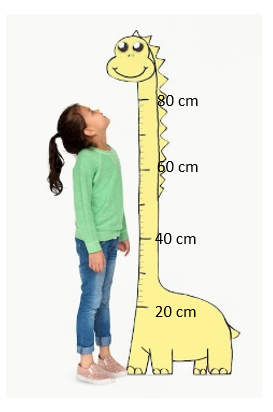
\includegraphics[width=1.67708in,height=2.53098in]{media/image21.png}

\conteudo{
MARIANA É UMA MENINA MUITO ESPERTA, QUE CRESCE DE FORMA SAUDÁVEL A CADA
ANO. SUA MÃE COLOU UMA MEDIDOR NA PAREDE DE SEU QUARTO, E A CADA ANO
ELAS ANOTAM A ALTURA DE MARIANA JUNTAS.

%\textless{}https://br.freepik.com/fotos-premium/escala-crescente-da-altura-alta-da-medida-da-crianca\_3375107.htm\#query=altura\%20de\%20crian\%C3\%A7a\&position=25\&from\_view=search\&track=ais. Favor colocar as cotas de altura.\textgreater{}

MARIANA ESTÁ AGORA COM 80 CENTÍMETROS DE \textbf{ALTURA}, QUE, EM GERAL, É A ALTURA DE UMA MESA DE ESCRITÓRIO.
ALÉM DISSO, A MÃE DE MARIANA TAMBÉM COMPROU UMA BALANÇA PARA MEDIR SEU
``PESO'' -- QUE, NA REALIDADE, É SUA MASSA. OBSERVE:

%\textless{}https://br.freepik.com/vetores-premium/ilustracao-em-escala-industrial-em-fundo-transparente\_23844742.htm\#query=balan\%C3\%A7a\%20digital\&position=37\&from\_view=search\&track=ais. Colocar o peso de Mariana em 18 kg.\textgreater{}

\begin{wrapfigure}{l}{.5\textwidth}
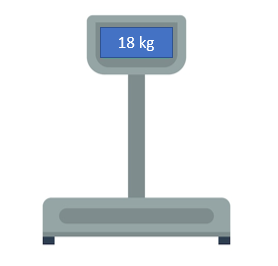
\includegraphics[width=.5\textwidth]{media/image22.png}
\end{wrapfigure}

MARIANA ESTÁ AGORA COM 18 QUILOGRAMAS DE \textbf{MASSA}, OU SEJA, A MESMA QUE UMA POLTRONA PODE TER. SE UMA POLTRONA E MARIANA TÊM A MESMA MASSA, POR QUE A POLTRONA É
TÃO MAIOR QUE MARIANA? CADA CORPO TEM UMA CAPACIDADE DIFERENTE DE OCUPAR
ESPAÇO. ESSA CAPACIDADE É O QUE CHAMAMOS DE \textbf{VOLUME}.

PARA MEDIRMOS COMPRIMENTOS, USAMOS A UNIDADE METROS, POR EXEMPLO. PARA MEDIRMOS MASSAS, USAMOS A MEDIDA
QUILOGRAMA, POR EXEMPLO. PARA MEDIRMOS O ESPAÇO OCUPADO, OU SEJA, O VOLUME, USAMOS
A MEDIDA LITRO, POR EXEMPLO.
}

\pagebreak
\colorsec{ATIVIDADES}

\num{1} CRICULE DE AZUL O QUE COMPRAMOS POR QUILOGRAMA (KG), DE VERDE O QUE
COMPRAMOS POR LITRO (L) E DE VERMELHO O QUE COMPRAMOS POR UNIDADE.\bigskip

%\textless{} https://br.freepik.com/vetores-premium/compra-de-mantimentos-frescos\_19552867.htm\#query=market\%20products\&position=9\&from\_view=search\&track=ais

\begin{minipage}{.5\textwidth}
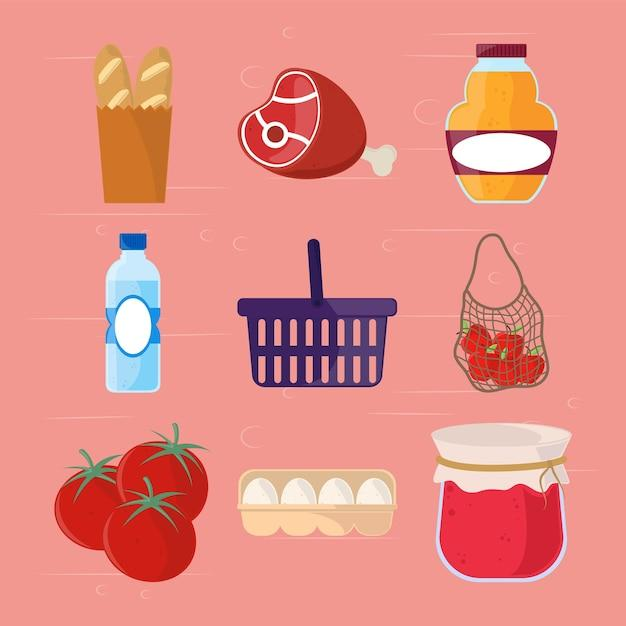
\includegraphics[width=\textwidth]{media/image23.jpg}
\end{minipage}\hspace{.5cm}
\sidetext{Oriente os alunos a se lembrarem das vezes em que foram ao
supermercado, por exemplo. Corrija a atividade com eles, mas permita que
eles tentem fazer sozinhos. Alguns dos itens são pedidos por unidades,
porém são pagos pela unidade de medidas, como é o caso dos pães. Se eles
colocarem na categoria do vendido por unidade, não considere erro, mas ressignifique, explicando
que, para o pagamento ser justo, é necessário que a cobrança seja feita, em alguns casos,
por quilograma ou litro. Assim, os alunos começam a perceber a real
importância das unidades de medida. Alguns alunos podem caracterizar a geleia como o vendido por litro. Se isso acontecer, explique
que somente líquidos são medidos assim e que massas pastosas são
medidas em quilogramas.}

\bigskip

\num{2} CIRCULE OS ITENS QUE PODEM SER MEDIDOS EM METROS.

%\textless{}Crie a figura conforme o modelo, utilizando as referências: https://br.freepik.com/vetores-premium/mesa-de-madeira\_31804490.htm\#query=mesa\%20desenho\&position=5\&from\_view=search\&track=ais; https://br.freepik.com/vetores-gratis/adesivo-de-pacote-de-saco-de-acucar-em-fundo-branco\_18055550.htm\#query=a\%C3\%A7ucar\%20desenho\&position=2\&from\_view=search\&track=ais (traduzir -- açúcar); https://br.freepik.com/vetores-gratis/fatia-de-queijo-saboroso\_3077481.htm\#query=queijo\%20desenho\&position=7\&from\_view=search\&track=ais; https://br.freepik.com/vetores-gratis/beber\_23715247.htm\#query=refri\%20desenho\&position=9\&from\_view=search\&track=ais; https://br.freepik.com/vetores-gratis/desenho-de-adesivo-com-rolo-de-corda-isolado\_18184169.htm\#query=cordadesenho\&position=0\&from\_view=search\&track=ais; \href{https://br.freepik.com/vetores-premium/oleo-de-motor-de-substituicao-mecanico-de-automoveis-segurando-uma-lata-de-oleo-de-motor-isolado-no-fundo-branco-manutencao-do-servico-da-estacao-motor-e-mecanismos-de-lubrificacao-design-plano-de-ilustracao-vetorial_23005619.htm\#query=gasolina\%20gal\%C3\%A3odesenho\&position=6\&from_view=search\&track=ais}{\emph{https://br.freepik.com/vetores-premium/oleo-de-motor-de-substituicao-mecanico-de-automoveis-segurando-uma-lata-de-oleo-de-motor-isolado-no-fundo-branco-manutencao-do-servico-da-estacao-motor-e-mecanismos-de-lubrificacao-design-plano-de-ilustracao-vetorial\_23005619.htm\#query=gasolina\%20gal\%C3\%A3odesenho\&position=6\&from\_view=search\&track=ais}}.\textgreater{} 

\begin{minipage}{.5\textwidth}
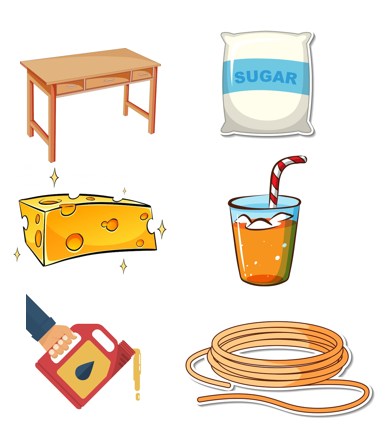
\includegraphics[width=\textwidth]{media/image24.png}
\end{minipage}\hspace{.5cm}
\sidetext{É importante que o aluno perceba que somente a mesa e a
corda podem ser medidas em metro.}

\pagebreak
\num{3} LIGUE CADA PRODUTO À UNIDADE MAIS ADEQUADA PARA MEDI-LO.

%\textless{}Inserir quadro conforme o modelo a seguir.\textgreater{}

\begin{figure}[htpb!]
\centering
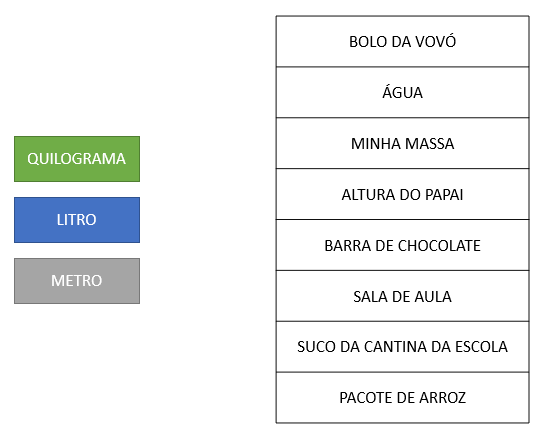
\includegraphics[width=4.86920in,height=3.96016in]{media/image25.png}
\end{figure}

\pagebreak
\num{4} EM CADA QUADRO A SEGUIR, DESENHE ALGO QUE POSSA SER MEDIDO COM O INSTRUMENTO REPRESENTADO.

%\textless{} insira os quadros e as figuras, conforme o modelo a seguir, utilizando as referências: https://br.freepik.com/vetores-premium/bonito-governante-engracado-acenando-o-personagem-de-mao\_23415941.htm\#page=3\&query=UMA\%20R\%C3\%89GUA\%20DESENHO\&position=39\&from\_view=search\&track=ais; https://br.freepik.com/vetores-gratis/balanca-digital-em-fundo-branco\_16262850.htm\#query=BALAN\%C3\%87A\%20DESENHO\&position=3\&from\_view=search\&track=ais; https://br.freepik.com/vetores-gratis/adesivo-de-copo-de-medicao-em-fundo-branco\_18180135.htm\#query=COPO\%20MEDIDORDESENHO\&position=2\&from\_view=search\&track=ais; https://br.freepik.com/vetores-premium/fita-metrica-para-medir-a-distancia-em-centimetros-e-milimetros-rabiscar-a-coloracao-linear-dos-desenhos-animados\_30247681.htm\#query=TRENA\%20DESENHO\&position=45\&from\_view=search\&track=ais.\textgreater{}

\begin{figure}[htpb!]
\centering
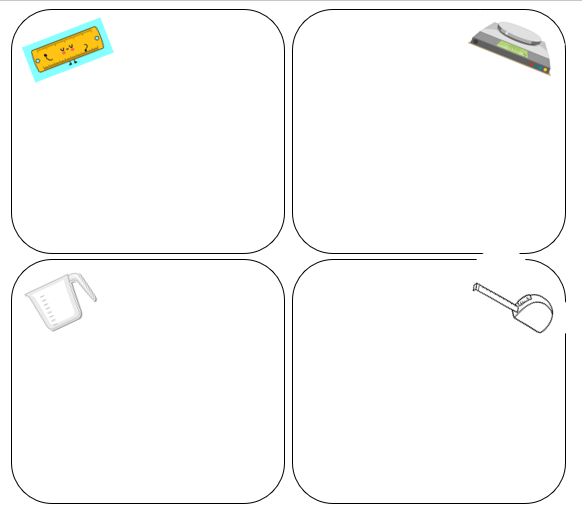
\includegraphics[width=6.43650in,height=5.62891in]{media/image26.png}
\end{figure}

\pagebreak
\num{5} LIGUE CADA PESSOA À SUA CAMA.

%\textless{}Crie um quadro conforme o modelo a seguir, utilizando as referências: https://br.freepik.com/vetores-premium/homem-segurando-binoculos-pessoa-olhando-para-o-horizonte-futuro\_30928646.htm\#query=adulto\%20alto\%20DESENHO\&position=6\&from\_view=search\&track=ais; https://br.freepik.com/vetores-premium/rapaz-dos-desenhos-animados-com-guitarra-criancas-tocando-instrumento-musical-em-casa-aula-ou-performance-artista-de-educacao-musical-ou-ferramentas-de-som-publicidade-vector-hobby-carreira-e-ilustracao-de-atividade-de-lazer\_26152103.htm\#query=adulto\%20baixo\%20DESENHO\&position=8\&from\_view=search\&track=ais; https://br.freepik.com/vetores-gratis/personagem-de-desenho-animado-de-menino-bonito-em-fundo-branco\_28457881.htm\#query=menino\%20DESENHO\&position=5\&from\_view=search\&track=ais; https://br.freepik.com/vetores-gratis/cama-com-travesseiro-e-lencol-azul\_2204447.htm\#query=cama\%20DESENHO\&position=1\&from\_view=search\&track=ais.\textgreater{}

\begin{figure}[htpb!]
\centering
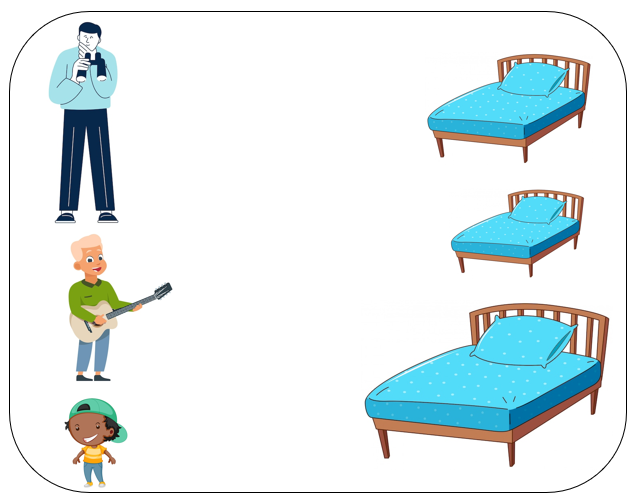
\includegraphics[width=6.28790in,height=4.93257in]{media/image27.png}
\end{figure}

\coment{É importante que o aluno reconheça que as diferenças de
altura entre as pessoas se reflete na diferença de tamanho das camas.
É assim que o aluno conseguirá inferir a medida de comprimento.}

\pagebreak
\num{6} PINTE COMO A JARRA MAIOR FICARIA SE FOR COLOCADO NELA TODO O LÍQUIDO DAS
JARRAS MENORES.

%\protect\hypertarget{_heading=h.gjdgxs}{}{}\textless{}Inserir a figura usando a referência: https://br.freepik.com/vetores-gratis/adesivo-de-copo-de-medicao-em-fundo-branco\_18180135.htm\#query=COPO\%20MEDIDORDESENHO\&position=2\&from\_view=search\&track=ais. Colocar as quantidades conforme o modelo a seguir.\textgreater{}

\begin{figure}[htpb!]
\centering
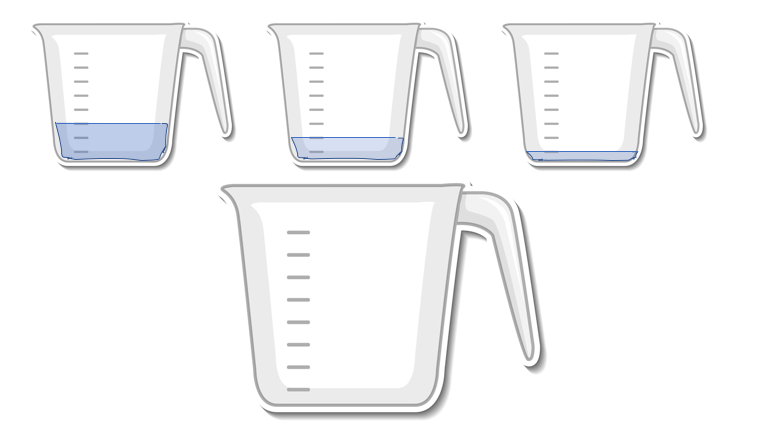
\includegraphics[width=5.90556in,height=3.37222in]{media/image28.png}
\end{figure}

\coment{É importante desenvolver nos alunos uma capacidade de
medição empírica, já que não existe a unidade precisa na jarra.
Oriente os alunos a contarem a quantidade de riscos das jarras. Eles
devem pintar até a sexta marcação.}

\num{7} AINDA SOBRE A ATIVIDADE ANTERIOR, SE CADA MARCAÇÃO DA JARRA MAIOR MEDIR MEIO LITRO,
QUANTOS LITROS TERIAM SIDO COLOCADOS NELA?

\reduline{3 litros.\hfill}


\num{8} QUAL É A CAPACIDADE TOTAL DA JARRA MAIOR DAS ATIVIDADES ANTERIORES? CONSIDERE, MAIS UMA VEZ, QUE CADA MARCAÇÃO CORRESPONDE A MEIO LITRO.

\reduline{4 litros.\hfill}

\pagebreak
\num{9} UTILIZE UMA RÉGUA E ESTIME O COMPRIMENTO DE CADA FIGURA A SEGUIR.

%\textless{}Inserir os quadros com as figuras conforme os modelos a
%seguir. Referências na figura.\textgreater{}
%
%\begin{longtable}[]{@{}l@{}}
%\toprule
%\begin{minipage}[t]{0.97\columnwidth}\raggedright\strut
\begin{figure}[htpb!]

\includegraphics[width=\textwidth]{media/image29.jpg}
\caption{MEDIDA:}
\end{figure}
% https://br.freepik.com/vetores-premium/icone-de-lapis-em-estilo-simples-ilustracao-vetorial-de-equipamentos-de-educacao-em-fundo-isolado-conceito-de-negocio-de-sinal-de-ferramenta-de-desenho\_30026502.htm\#%query=lapis\&position=6\&from\_view=search\&track=sph\strut
%\end{minipage}\tabularnewline
%medida:\tabularnewline
%\bottomrule
%\end{longtable}
%
%\begin{longtable}[]{@{}l@{}}
%\toprule
%\begin{minipage}[t]{0.97\columnwidth}\raggedright\strut
\begin{figure}[htpb!]
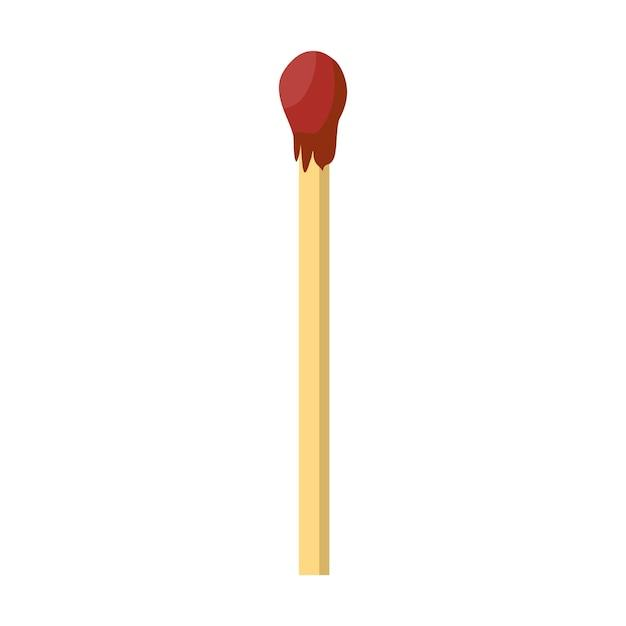
\includegraphics[width=.5\textwidth]{media/image30.jpg}
\caption{MEDIDA:}
\end{figure}
% https://br.freepik.com/vetores-premium/objetos-vetoriais-isolados-de-desenho-animado-combinam-e-fogo\_29291308.htm\#query=palito\%20de\%20f\%C3\%B3sforo\%20desenho\&position=9\&from\_view=search\&track=ais\%strut
%\end{minipage}\tabularnewline
%medida:\tabularnewline
%\bottomrule
%\end{longtable}
%
%\begin{longtable}[]{@{}l@{}}
%\toprule
%\begin{minipage}[t]{0.97\columnwidth}\raggedright\strut
\begin{figure}[htpb!]
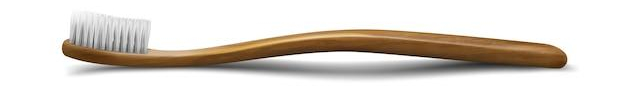
\includegraphics[width=.9\textwidth]{media/image31.jpg}
\caption{MEDIDA:}
\end{figure}
% https://br.freepik.com/vetores-premium/objetos-vetoriais-isolados-de-desenho-animado-combinam-e-fogo\_29291308.htm\#query=palito\%20de\%20f\%C3\%B3sforo\%20desenho\&position=9\&from\_view=search\&track=ais\%strut
%\end{minipage}\tabularnewline
%medida:\tabularnewline
%\bottomrule
%\end{longtable}

\coment{Oriente os alunos quanto ao fato de suas réguas medirem
comprimentos menores do que um metro. Explique que o centímetro
é uma subdivisão dessa unidade de medida. Este não é o momento de quantificar essa subdivisão.
Basta que entendam que se trata de outra unidade para medir
comprimentos.}

\pagebreak
\colorsec{TREINO}

\num{1} COMPARE AS ALTURAS DAS CRIANÇAS REPRESENTADAS A SEGUIR.

%\textless{} https://br.freepik.com/vetores-gratis/quatro-criancas\_4906544.htm\#page=2\&query=crian\%C3\%A7as\%20com\%20diferentes\%20alturas\%20desenho\&position=13\&from\_view=search\&track=ais.\textgreater{}

\begin{figure}[htpb!]
\centering
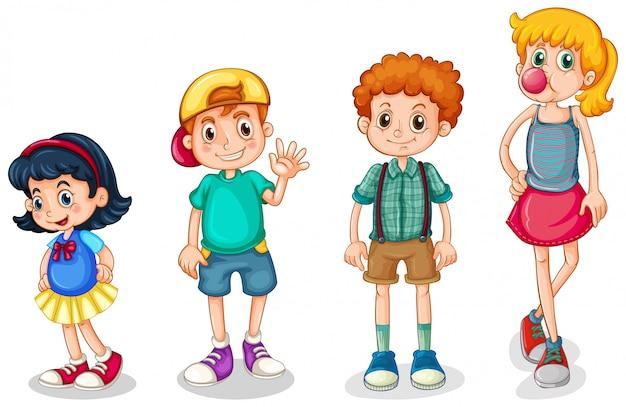
\includegraphics[width=4.23198in,height=2.75148in]{media/image32.jpg}
\end{figure}

A CRIANÇA MAIS ALTA É

\begin{escolha}
\item A MENINA DE SAIA AMARELA.

\item A MENINA MASCANDO GOMA.

\item O MENINO DE BONÉ.

\item O MENINO DE TÊNIS AZUL.
\end{escolha}

\coment{SAEB: Comparar comprimentos, capacidades ou massas ou ordenar
imagens de objetos com base na comparação visual de seus comprimentos,
capacidades ou massas.
BNCC: EF01MA15 -- Comparar comprimentos, capacidades ou massas,
utilizando termos como mais alto, mais baixo, mais comprido, mais curto,
mais grosso, mais fino, mais largo, mais pesado, mais leve, cabe mais,
cabe menos, entre outros, para ordenar objetos de uso cotidiano.}



\num{2} OBSERVE ESTA IMAGEM:

\begin{figure}[htpb!]
\centering
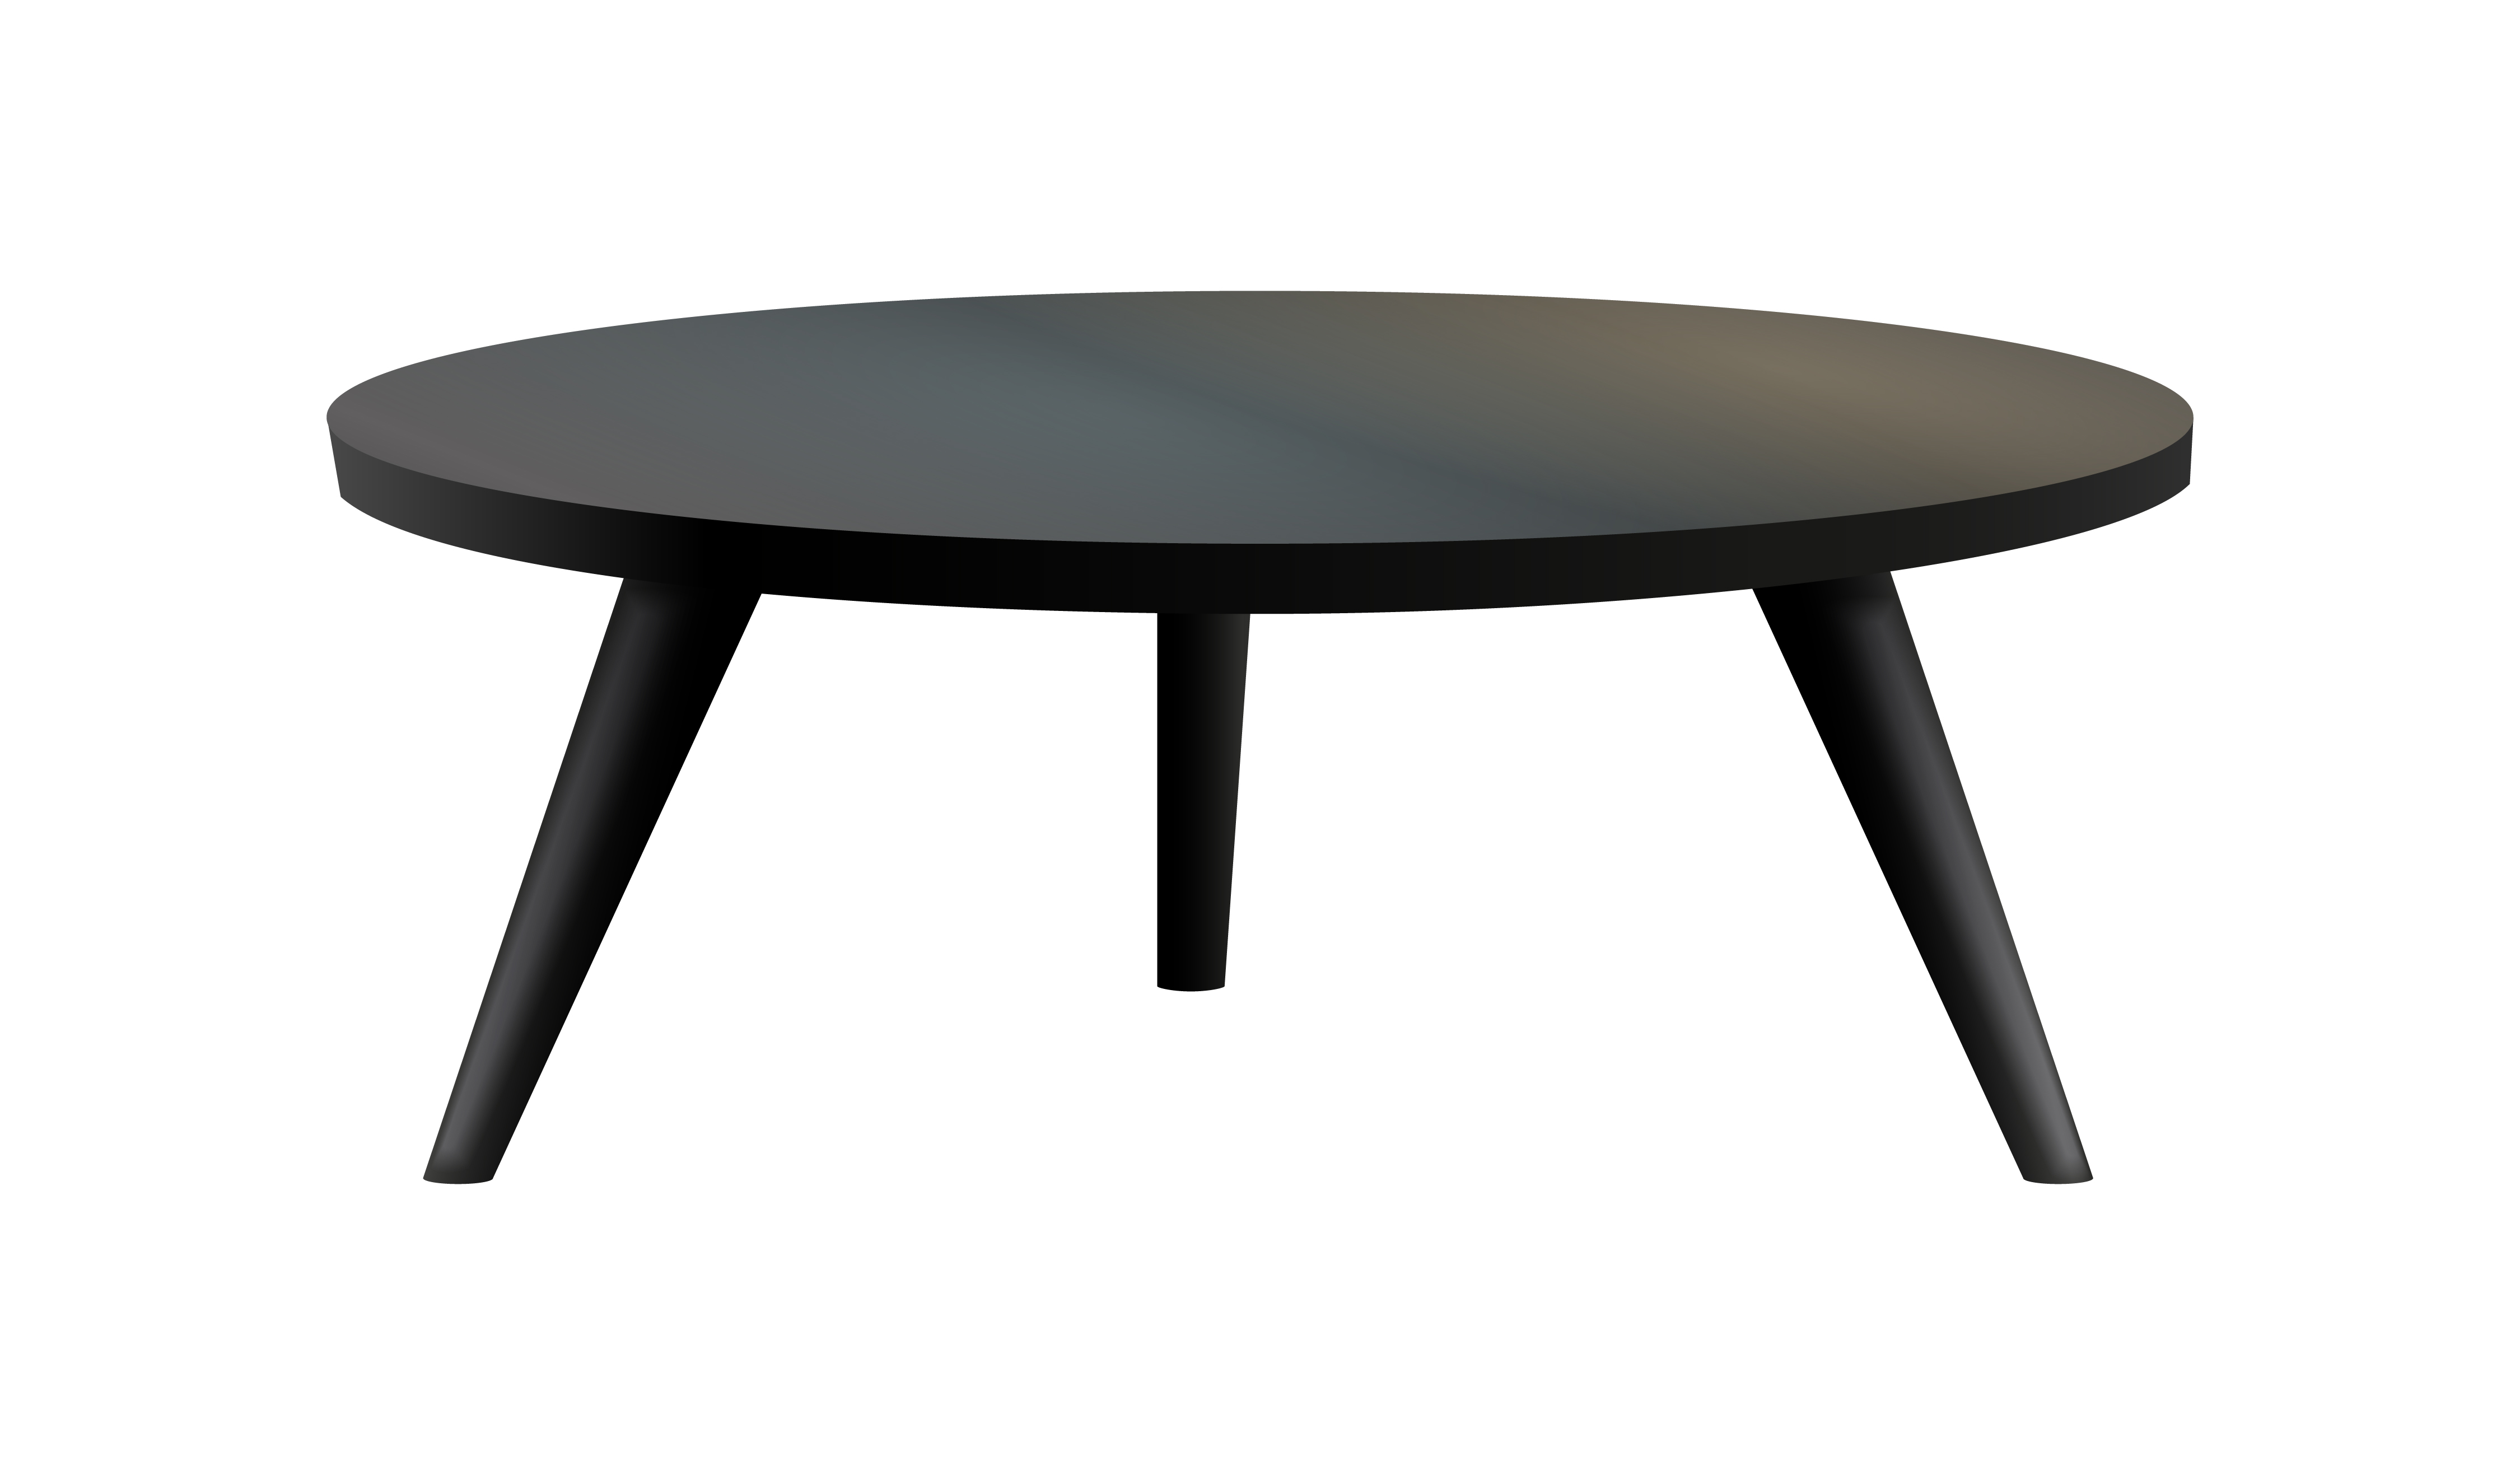
\includegraphics[width=.5\textwidth]{media/image32b.jpg}
\end{figure}

QUAL DESTES É O MELHOR INSTRUMENTO DE MEDIDA PARA SE MEDIR A DISTÂNCIA DO TAMPO DA MESA ATÉ O CHÃO?

\begin{escolha}
\item UMA BALANÇA

\item UM COPO DE MEDIÇÃO.

\item UMA RÉGUA.

\item UMA PANELA.
\end{escolha}

\coment{SAEB: Reconhecer unidades de medida e/ou instrumentos utilizados
para medir comprimento, tempo, massa ou capacidade.
BNCC: EF01MA15 -- Comparar comprimentos, capacidades ou massas,
utilizando termos como mais alto, mais baixo, mais comprido, mais curto,
mais grosso, mais fino, mais largo, mais pesado, mais leve, cabe mais,
cabe menos, entre outros, para ordenar objetos de uso cotidiano.}


\num{3} VEJA A IMAGEM.

%\textless{}https://br.freepik.com/fotos-gratis/closeup-de-peso-escalas-conceito-de-excesso-de-peso-e-obesidade\_3219089.htm\#page=5\&query=regua\%20medindo\&position=49\&from\_view=search\&track=ais\textgreater{}

\begin{figure}[htpb!]
\centering
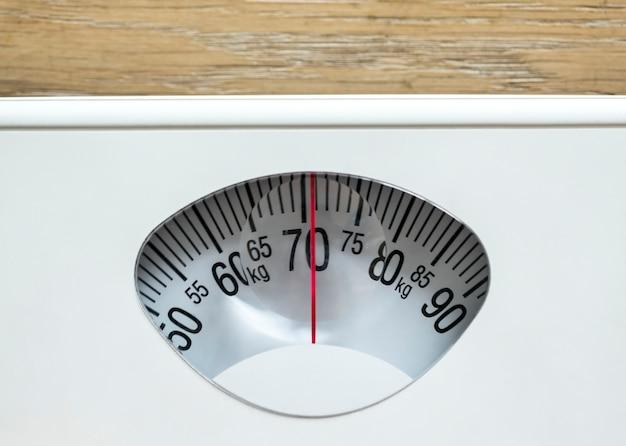
\includegraphics[width=3.03770in,height=1.48580in]{media/image33.jpg}
\end{figure}

NA IMAGEM, MOSTRA-SE A MEDIÇÃO DA MASSA DA MÃE DE JULIANA NO VISOR DA
BALANÇA. QUAL É A MASSA DA MÃE DE JULIANA, MEDIDA EM QUILOGRAMAS?

\begin{escolha}
\item 69.

\item 70.

\item 71.

\item 72.
\end{escolha}

\coment{SAEB: Identificar a medida de comprimento, da capacidade ou da
massa de objetos, dada a imagem de um instrumento de medida.
BNCC: EF01MA15 -- Comparar comprimentos, capacidades ou massas,
utilizando termos como mais alto, mais baixo, mais comprido, mais curto,
mais grosso, mais fino, mais largo, mais pesado, mais leve, cabe mais,
cabe menos, entre outros, para ordenar objetos de uso cotidiano.}

\chapter{EM QUE DIA DA SEMANA CAI MEU ANIVERSÁRIO?}
\markboth{Módulo 4}{}

\coment{Neste módulo, vamos desenvolver nos alunos a habilidade de orientar-se no
tempo, sabendo identificar o tempo presente, assim como prever dias e
horários de eventos futuros.\\
Habilidades da BNCC EF01MA16, EF01MA17, EF01MA18.}

\colorsec{Habilidades do SAEB}

\begin{itemize}
\item Identificar sequência de acontecimentos relativos a um dia.
\item Identificar datas, dias da semana ou meses do ano em calendário ou
escrever uma data, apresentando o dia, o mês e o ano.
\item Determinar a data de início, a data de término ou a duração de um
acontecimento entre duas datas.
\item Determinar o horário de início, o horário de término ou a duração de
um acontecimento.
\end{itemize}

\conteudo{\begin{wrapfigure}{l}{.5\textwidth}
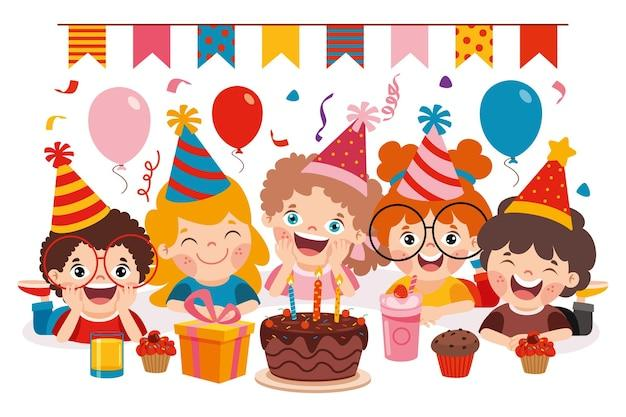
\includegraphics[width=.5\textwidth]{media/image34.jpg}
\end{wrapfigure}

É COMUM AS PESSOAS FICAREM ANSIOSAS PARA CHEGAR O DIA DO PRÓPRIO ANIVERSÁRIO!
NÃO VEMOS A HORA DE GANHAR PRESENTES, COMER BOLO, ASSOPRAR A VELA E
FICAR COM OS AMIGOS. VOCÊ SABE EM QUE DIA ISSO ACONTECERÁ? E EM QUE DIA
DA SEMANA? VOCÊ SABE DIZER A QUE HORAS VAI COMEÇAR OU TERMINAR A 
FESTA DE ANIVERSÁRIO?

%\textless{}https://br.freepik.com/vetores-premium/personagens-de-desenhos-animados-comemorando-a-festa-de-aniversario\_28760759.htm\#query=festa\%20de\%20aniversario\%20crian\%C3\%A7as\&position=10\&from\_view=search\&track=ais\textgreater{}

VAMOS LEMBRAR COMO É ORGANIZADO NOSSO CALENDÁRIO.

O ANO É DIVIDIDO EM 365 DIAS, E CADA DIA TEM 24 HORAS. ALÉM DISSO, O ANO
TAMBÉM É DIVIDIDO EM 12 MESES, E OS MESES TÊM ENTRE 28 E 31 DIAS. VOCÊ LEMBRA O NOME DOS MESES E A QUANTIDADE
DE DIAS DE CADA UM? OBSERVE:

%{\footnotesize
%\begin{longtable}[]{@{}llllll@{}}
%\toprule
%\textbf{JANEIRO} & \textbf{FEVEREIRO} & \textbf{MARÇO} & \textbf{ABRIL} & \textbf{MAIO} & \textbf{JUNHO}\%tabularnewline
%31 DIAS & 28/29 DIAS & 31 DIAS & 30 DIAS & 31 DIAS & 30 DIAS\tabularnewline
%\textbf{JULHO} & \textbf{AGOSTO} & \textbf{SETEMBRO} & \textbf{OUTUBRO} & \textbf{NOVEMBRO} & \textbf{%DEZEMBRO}\tabularnewline
%31 DIAS & 31 DIAS & 30 DIAS & 31 DIAS & 30 DIAS & 31 DIAS\tabularnewline
%\bottomrule
%\end{longtable}
%}

\begin{center}
\begin{tabular}{ll}
\textbf{JANEIRO} & 31 DIAS \\
\textbf{FEVEREIRO} & 28/29 DIAS \\
\textbf{MARÇO} & 31 DIAS \\
\textbf{ABRIL} & 30 DIAS \\
\textbf{MAIO} & 31 DIAS \\
\textbf{JUNHO} &30 DIAS\\
\textbf{JULHO} & 31 DIAS \\
\textbf{AGOSTO} & 31 DIAS \\
\textbf{SETEMBRO} & 30 DIAS \\
\textbf{OUTUBRO} & 31 DIAS \\
\textbf{NOVEMBRO} & 30 DIAS \\
\textbf{DEZEMBRO} & 31 DIAS\\
\end{tabular}
\end{center}

OS MESES ESTÃO ORGANIZADOS EM SEMANAS, QUE SÃO DIVIDIDAS EM 7 DIAS. OBSERVE OS NOMES
DESSES DIAS:

\begin{mdframed}[linewidth=2pt,linecolor=salmao,roundcorner=10pt]
DOMINGO \hfill SEGUNDA-FEIRA \hfill TERÇA-FEIRA \hfill QUARTA-FEIRA \hfill QUINTA-FEIRA \hfill SEXTA-FEIRA \hfill
SÁBADO
\end{mdframed}
}

\pagebreak
\colorsec{ATIVIDADES}

\num{1} VAMOS DESCOBRIR QUE DIA É HOJE? ESCREVA O QUE SE PEDE A SEGUIR.

\begin{escolha}
\item Em que ano estamos? \reduline{\mbox{}\hfill}

\item Em que mês estamos? \reduline{\mbox{}\hfill}

\item Que dia do mês é hoje? \reduline{\mbox{}\hfill}

\item Que dia da semana é hoje? \reduline{\mbox{}\hfill}

\item Que horas são neste momento em que você está resolvendo esta atividade? \reduline{\mbox{}\hfill}
\end{escolha}

\coment{O mais importante nesta atividade é fazer com que o aluno
consiga diferenciar cada classificação do tempo, como saber diferenciar dia
do mês e dia da semana, por exemplo. Oriente-os a preencherem o horário
com horas, minutos e segundos. Essa atividade pode e deve ser usada com
fins de avaliação diagnóstica.}

\num{2} PINTE OS QUADRADOS COM A COR EQUIVALENTE.

\begin{center}
{\large
\begin{tabular}{|c|c|c|c|c|}
\hline
\textcolor{blue}{\textbf{Domingo}} & \textcolor{green}{\textbf{30}} & \textcolor{yellow}{\textbf{Março}} & \textcolor{red}{\textbf{2022}} & \textcolor{orange}{\textbf{13:15:00}} \\ \hline
mês & ano & horário & dia do mês & dia da semana \\ \hline
\end{tabular}
}
\end{center}

\coment{A sequência de cores é: amarelo, vermelho, laranja, verde e azul.}

\pagebreak
\num{3} CIRCULE NO CALENDÁRIO O DIA DO SEU ANIVERSÁRIO E ANOTE EM QUE DIA DA SEMANA ELE ESTÁ.

%\textless{} https://br.freepik.com/vetores-premium/calendario-de-cores-para-2023-com-um-coelho-de-personagem-fofo-a-semana-comeca-no-domingo-diversao-e-estilo-de-desenho-animado-de-design-brilhante\_34560382.htm\#query=calend\%C3\%A1rio\%20infantil\%202023\%20em\%20portugu\%C3\%AAs\&position=6\&from\_view=search\&track=ais. Traduzir os nomes dos meses, além das iniciais dos dias da semana.\textgreater{} 

\begin{figure}[htpb!]
\centering
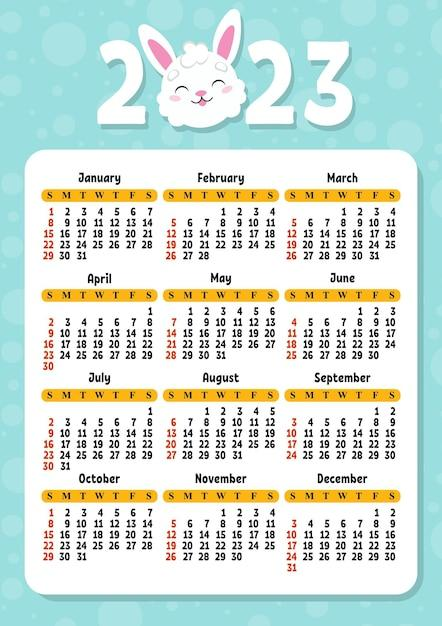
\includegraphics[width=4.71050in,height=6.67143in]{media/image35.jpg}
\end{figure}


\pagebreak
\num{4} ANALISE AS FIGURAS E LISTE A ORDEM DOS ACONTECIMENTOS EM UM DIA.

%\textless{}Inserir as figuras na ordem do modelo a seguir. Utilizar as referências: https://br.freepik.com/vetores-premium/garoto-bonito-comendo-delicioso-arroz-frito\_35549113.htm\#query=crian\%C3\%A7a\%20almo\%C3\%A7ando\&position=48\&from\_view=search\&track=ais; https://br.freepik.com/vetores-gratis/menino-dormir-cama\_4388324.htm\#query=crian\%C3\%A7a\%20acordando\&position=21\&from\_view=search\&track=ais; https://br.freepik.com/vetores-gratis/menino-que-dorme-na-cama\_1021842.htm\#query=crian\%C3\%A7a\%20acordando\&position=23\&from\_view=search\&track=ais; https://br.freepik.com/vetores-gratis/uma-garota-fazendo-o-exame\_2607446.htm\#query=crian\%C3\%A7a\%20estudasndo\&position=0\&from\_view=search\&track=ais e https://br.freepik.com/vetores-gratis/criancas-felizes-brincando-com-brinquedos\_11575551.htm\#query=crian\%C3\%A7a\%20brincando\&position=32\&from\_view=search\&track=ais \textgreater{}

\begin{figure}[htpb!]
\centering
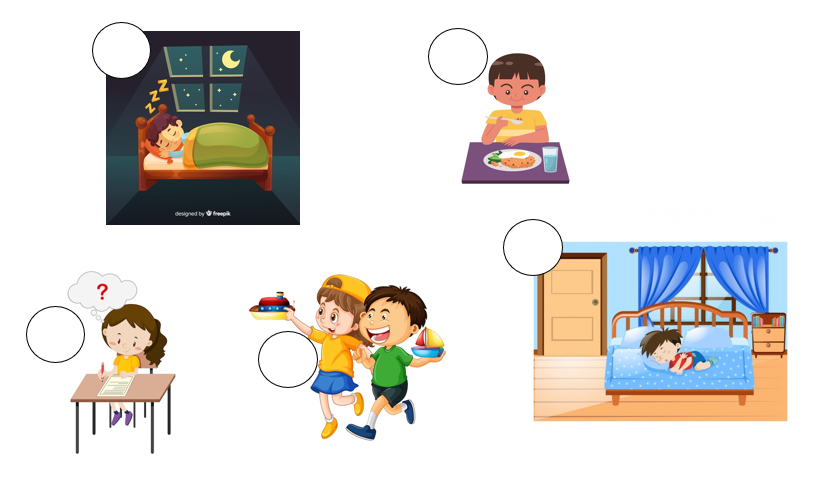
\includegraphics[width=5.90556in,height=3.46597in]{media/image36.png}
\end{figure}

\coment{Espera-se que os alunos sigam a ordem dos acontecimentos
baseando-se nas próprias rotinas. Aproveite para frisar a importância de
se alimentar no horário certo, além de
ressaltar a importância de priorizar o momento dos estudos, ou seja,
estudar antes de brincar. Esta atividade pode ser utilizada também para
os alunos lembrarem a utilização dos números para ordenar.
Oriente-os a utilizarem os números de forma ordinal (1º, 2º, 3º etc.).}

\num{5} COMPLETE OS QUADRADOS EM BRANCO DO CALENDÁRIO A SEGUIR.

\begin{center}
{\large
\begin{tabular}{|ccccccc|}
\hline
\multicolumn{7}{|c|}{\textbf{JANEIRO 2023}} \\ \hline
\multicolumn{1}{|c|}{\textbf{DOM}} & \multicolumn{1}{c|}{\rosa{2ª feira}} & \multicolumn{1}{c|}{\textbf{3ª FEIRA}} & \multicolumn{1}{c|}{\rosa{4ª feira}} & \multicolumn{1}{c|}{\textbf{5ª FEIRA}} & \multicolumn{1}{c|}{\textbf{6ª FEIRA}} & \rosa{Sábado} \\ \hline
\multicolumn{1}{|c|}{1} & \multicolumn{1}{c|}{2} & \multicolumn{1}{c|}{3} & \multicolumn{1}{c|}{\rosa{4}} & \multicolumn{1}{c|}{5} & \multicolumn{1}{c|}{\rosa{6}} & 7 \\ \hline
\multicolumn{1}{|c|}{8} & \multicolumn{1}{c|}{9} & \multicolumn{1}{c|}{\rosa{10}} & \multicolumn{1}{c|}{11} & \multicolumn{1}{c|}{\rosa{12}} & \multicolumn{1}{c|}{13} & 14 \\ \hline
\multicolumn{1}{|c|}{\rosa{15}} & \multicolumn{1}{c|}{16} & \multicolumn{1}{c|}{17} & \multicolumn{1}{c|}{18} & \multicolumn{1}{c|}{19} & \multicolumn{1}{c|}{20} & 21 \\ \hline
\multicolumn{1}{|c|}{22} & \multicolumn{1}{c|}{23} & \multicolumn{1}{c|}{24} & \multicolumn{1}{c|}{\rosa{25}} & \multicolumn{1}{c|}{26} & \multicolumn{1}{c|}{27} & \rosa{28} \\ \hline
\multicolumn{1}{|c|}{29} & \multicolumn{1}{c|}{30} & \multicolumn{1}{c|}{31} & \multicolumn{1}{c|}{} & \multicolumn{1}{c|}{} & \multicolumn{1}{c|}{} &  \\ \hline
\end{tabular}
}
\end{center}

\coment{Os alunos devem preencher os quadrados faltantes dos
dias do mês, assim como dos dias da semana.}

\pagebreak
\num{6} BASEANDO-SE NO CALENDÁRIO DA ATIVIDADE ANTERIOR, RESPONDA AO QUE SE PERGUNTA A SEGUIR.

\begin{escolha}
\item EM QUE DIA DA SEMANA ESTÁ O DIA 18 DE JANEIRO?

\reduline{Quarta-feira.\hfill}

\item QUANTOS SÁBADOS EXISTEM EM JANEIRO DE 2023?

\reduline{São quatro sábados.\hfill}

\item EM QUE DIA DA SEMANA COMEÇA ESSE MÊS DE JANEIRO?

\reduline{Domingo.\hfill}

\item EM QUE DIA DA SEMANA TERMINA ESSE MÊS DE JANEIRO?

\reduline{Terça-feira.\hfill}

\item QUANTOS DOMINGOS EXISTEM NESSE MÊS DE JANEIRO?

\reduline{São cinco domingos.\hfill}
\end{escolha}

\coment{Aproveite para demonstrar que, em alguns meses,
pode haver algum dia da semana se repetindo cinco vezes, ou seja, o fato de
haver quatro semanas em um mês não significa que haverá sempre quatro repetições
de cada dia da semana. Esta atividade é importante para desenvolver no
aluno a habilidade de ler o calendário com entendimento.}

\num{7} ANALISE O BLOCO DE NOTAS DE MARCELA. QUANTOS DIAS ELA ESPERARÁ
PELA RESPOSTA DE QUE PRECISA?

%\textless{}Inserir a figura da referência: https://br.freepik.com/vetores-premium/caderno-e-lapis-em-fundo-branco\_10079541.htm\#query=bloco\%20de\%20anota\%C3\%A7\%C3\%B5es\&position=10\&from\_view=search\&track=ais, incluindo o texto conforme o modelo:\textgreater{}

\begin{figure}[htpb!]
\centering
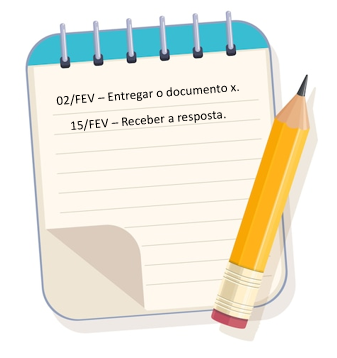
\includegraphics[width=.5\textwidth]{media/image37.png}
\end{figure}

\reduline{Entre os dias 2 e 15, passam-se 13 dias.\hfill}

\num{8} SE O DIA DA SEMANA EM QUE MARCELA ENTREGOU O DOCUMENTO FOSSE
SEXTA-FEIRA, EM QUE DIA DA SEMANA CAIRIA O DIA DA RESPOSTA?

\reduline{Quinta-feira.\hfill}

\num{9} EM UMA ESCOLA, UMA COMPETIÇÃO DE FUTEBOL DE SALÃO DUROU SETE DIAS.
SE A COMPETIÇÃO COMEÇOU NO DIA 10 DE OUTUBRO DE 2021, UM SÁBADO, EM QUE
DATA TERMINOU O CAMPEONATO?

\begin{itemize}
\item ANO: \reduline{2021\hfill}

\item MÊS: \reduline{Outubro\hfill}

\item DIA DO MÊS: \reduline{16\hfill}

\item DIA DA SEMANA: \reduline{Sexta-feira\hfill}
\end{itemize}


\num{10} ANALISE OS RELÓGIOS DIGITAIS DA IMAGEM. DEPOIS, RESPONDA AO QUE SE PERGUNTA A SEGUIR.

%\textless{}Inserir a figura da referência: https://br.freepik.com/vetores-premium/um-conjunto-de-relogios-digitais-numeros-eletronicos-ilustracao-vetorial\_32708528.htm\#query=rel\%C3\%B3gio\%20digital\&position=16\&from\_view=search\&track=ais, inserindo as identificações dos relógios, conforme o modelo a seguir.\textgreater{}

\begin{figure}[htpb!]
\centering
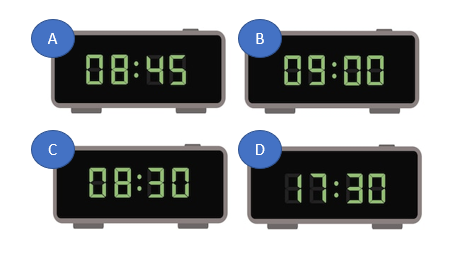
\includegraphics[width=.5\textwidth]{media/image38.png}
\end{figure}

\begin{escolha}
\item QUAL É A DIFERENÇA ENTRE O HORÁRIO DO RELÓGIO \textbf{A} E O DO RELÓGIO \textbf{B}?

\reduline{Uma hora e quarenta e cinco minutos. 01:45:00.\hfill}

\item QUAL É A DIFERENÇA ENTRE O HORÁRIO DO RELÓGIO \textbf{C} E O DO RELÓGIO \textbf{A}?

\reduline{Quinze minutos. 00:15:00.\hfill}

\item QUAL É A DIFERENÇA ENTRE O HORÁRIO DO RELÓGIO \textbf{B} E O DO RELÓGIO \textbf{D}?

\reduline{Oito horas e trinta minutos. 08:30:00.\hfill}

\item QUAL É A DIFERENÇA ENTRE O HORÁRIO DO RELÓGIO \textbf{C} E O DO RELÓGIO \textbf{D}?

\reduline{Nove horas. 09:00:00.\hfill}
\end{escolha}

\coment{Oriente os alunos a darem respostas neste formato: hh:mm:ss.}

\num{11} PARA ACORDAR, MARIANO AJUSTOU O ALARME DO CELULAR PARA O HORÁRIO MOSTRADO A SEGUIR.\bigskip

%\textless{}https://br.freepik.com/vetores-gratis/smartphone-de-tela-de-alarme\_2921841.htm\#query=relogio\%20celular\&position=48\&from\_view=search\&track=ais.\textgreater{}

\begin{minipage}{.5\textwidth}
\centering
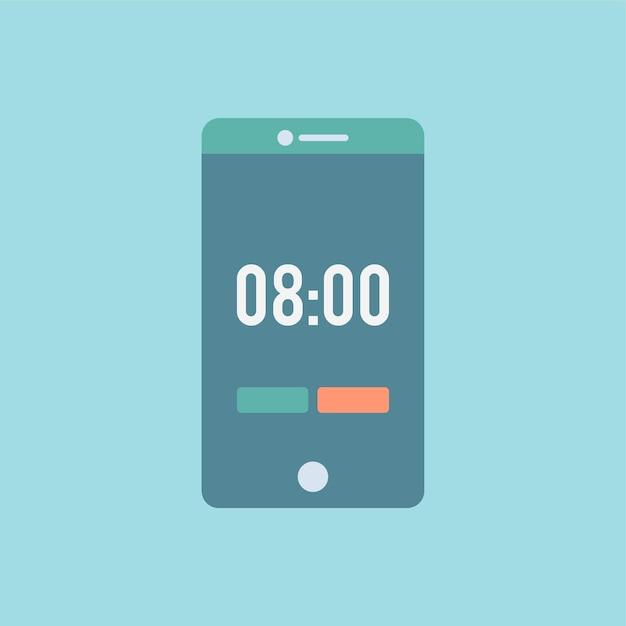
\includegraphics[width=.5\textwidth]{media/image39.jpg}
\end{minipage}\hspace{.5cm}
\begin{minipage}{.5\textwidth}
ELE LEVANTOU-SE, ARRUMOU-SE, TOMOU CAFÉ DA MANHÃ E FOI PARA O TRABALHO. CHEGOU AO TRABALHO 1 HORA E 35 MINUTOS DEPOIS DE ACORDAR. A QUE HORAS ELE CHEGOU AO TRABALHO?
\end{minipage}\bigskip\bigskip

\reduline{09:35:00.\hfill}

\num{12} PEDRO ACORDOU ÀS 07:30 DA MANHÃ.

%https://br.freepik.com/vetores-gratis/um-menino-dormindo-profundamente\_23807622.htm\#query=PEDRINHO\%20ACORDANDO\&position=5\&from\_view=search\&track=ais.\textgreater{}; https://br.freepik.com/vetores-gratis/menino-de-pijama-segurando-a-escova-de-dentes-e-pasta-de-dente\_27547013.htm\#query=ESCOVAR\%20OS\%20DENTES\&position=32\&from\_view=search\&track=ais https://br.freepik.com/vetores-gratis/um-menino-feliz-comendo-na-mesa\_18973385.htm\#query=CAF\%C3\%81\%20DA\%20MANH\%C3\%83\%20MENINO\&position=12\&from\_view=search\&track=ais; https://br.freepik.com/vetores-premium/um-menino-brincando-com-gato-fofo\_29183474.htm\#page=2\&query=BRINCANDO\%20COM\%20O\%20GATO\&position=6\&from\_view=search\&track=ais. \textgreater{} \begin{quote} 

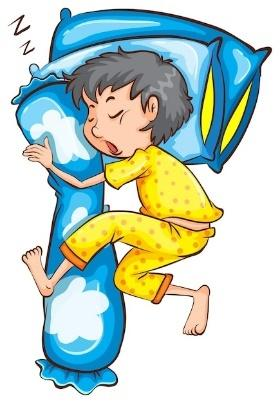
\includegraphics[width=1.27248in,height=1.83120in]{media/image40.jpg}
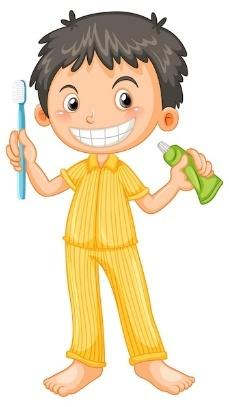
\includegraphics[width=1.04250in,height=1.85399in]{media/image41.jpg}
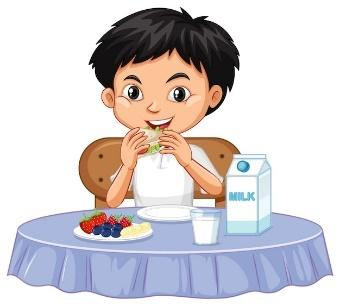
\includegraphics[width=1.54748in,height=1.39171in]{media/image42.jpg}
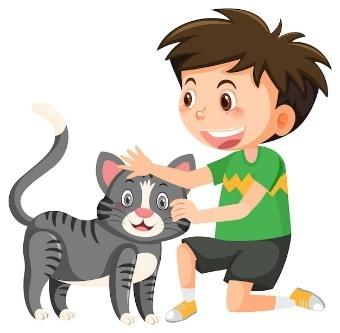
\includegraphics[width=1.54490in,height=1.51274in]{media/image43.jpg}

DEPOIS, DEMOROU 15 MINUTOS PARA IR AO BANHEIRO E ESCOVAR OS DENTES.
DEMOROU MAIS 20 MINUTOS PARA TOMAR O CAFÉ DA MANHÃ. ANTES DE SAIR,
AINDA FICOU 5 MINUTOS BRINCANDO COM O GATO. ENTÃO SAIU PARA A ESCOLA.

PINTE NO RELÓGIO A SEGUIR O HORÁRIO EM QUE PEDRO SAIU PARA IR À ESCOLA.

%\textless{}Inserir uma figura de um relógio, com os números em branco para o aluno preencher, conforme o modelo a seguir:\textgreater{}

\begin{figure}[htpb!]
\centering

\includegraphics[width=.8\textwidth]{media/image44.png}
\end{figure}

\coment{Oriente os alunos a pintarem os quadradinhos para formar o
horário, da mesma forma como aparecem nos relógios digitais. A pintura
deve formar o horário 08:10:00}

\pagebreak
\colorsec{TREINO}

\num{1} ANALISE O CALENDÁRIO A SEGUIR.

\begin{center}
\begin{tabular}{|ccccccc|}
\hline
\multicolumn{7}{|c|}{\textbf{FEVEREIRO 2023}} \\ \hline
\multicolumn{1}{|c|}{\textbf{DOM}} & \multicolumn{1}{c|}{\textbf{2ª FEIRA}} & \multicolumn{1}{c|}{\textbf{3ª FEIRA}} & \multicolumn{1}{c|}{\textbf{4ª FEIRA}} & \multicolumn{1}{c|}{\textbf{5ª FEIRA}} & \multicolumn{1}{c|}{\textbf{6ª FEIRA}} & \textbf{SÁBADO} \\ \hline
\multicolumn{1}{|c|}{} & \multicolumn{1}{c|}{} & \multicolumn{1}{c|}{} & \multicolumn{1}{c|}{1} & \multicolumn{1}{c|}{2} & \multicolumn{1}{c|}{3} & 4 \\ \hline
\multicolumn{1}{|c|}{5} & \multicolumn{1}{c|}{6} & \multicolumn{1}{c|}{7} & \multicolumn{1}{c|}{8} & \multicolumn{1}{c|}{9} & \multicolumn{1}{c|}{10} & 11 \\ \hline
\multicolumn{1}{|c|}{12} & \multicolumn{1}{c|}{13} & \multicolumn{1}{c|}{14} & \multicolumn{1}{c|}{15} & \multicolumn{1}{c|}{16} & \multicolumn{1}{c|}{17} & 18 \\ \hline
\multicolumn{1}{|c|}{19} & \multicolumn{1}{c|}{20} & \multicolumn{1}{c|}{21} & \multicolumn{1}{c|}{22} & \multicolumn{1}{c|}{23} & \multicolumn{1}{c|}{24} & 25 \\ \hline
\multicolumn{1}{|c|}{26} & \multicolumn{1}{c|}{27} & \multicolumn{1}{c|}{28} & \multicolumn{1}{c|}{} & \multicolumn{1}{c|}{} & \multicolumn{1}{c|}{} &  \\ \hline
\end{tabular}
\end{center}

A ÚLTIMA SEGUNDA-FEIRA DESSE MÊS SERÁ O DIA

\begin{minipage}{.5\textwidth}
\begin{escolha}
\item 6.

\item 26.

\item 27.

\item 28.
\end{escolha}
\end{minipage}
\sidetext{SAEB: Identificar datas, dias da semana ou meses do ano em
calendário ou escrever uma data, apresentando o dia, o mês e o ano.
BNCC: EF01MA17 -- Reconhecer e relacionar períodos do dia, dias da semana
e meses do ano, utilizando calendário, quando necessário.}


\num{2} ANALISE AS FIGURAS E INDIQUE QUAL É A SEQUÊNCIA CORRETA DE
ACONTECIMENTOS.

%\textless{}https://br.freepik.com/vetores-gratis/antecedentes-da-paisagem-plana-em-tons-roxos\_1001699.htm\#query=anoitecer\&position=2\&from\_view=search\&track=sph; https://br.freepik.com/vetores-gratis/paisagem-do-por-do-sol-com-lago-nuvens-no-ceu-vermelho-silhuetas-nas-colinas-e-arvores-na-costa\_12407808.htm\#query=amanhecer\&position=1\&from\_view=search\&track=sph

%; https://br.freepik.com/vetores-gratis/paisagem-de-primavera-desenhados-a-mao\_6804642.htm\#query=meio\%20dia\%20paisagem\&position=13\&from\_view=search\&track=ais

%; https://br.freepik.com/vetores-gratis/lua-cheia-noite-oceano-cartoon-ilustracao\_6690817.htm\#query=noite\%20paisagem\&position=10\&from\_view=search\&track=ais

\begin{figure}[htpb!]
\centering
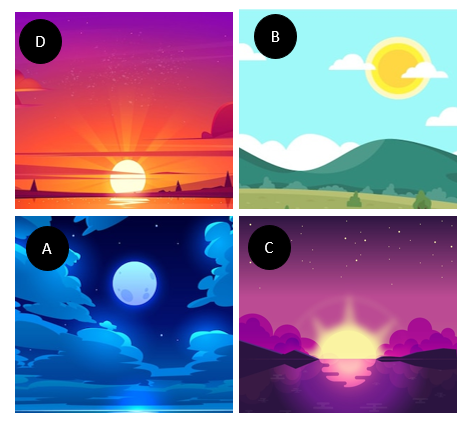
\includegraphics[width=.7\textwidth]{media/image46.png}
\end{figure}

\begin{minipage}{.5\textwidth}
\begin{escolha}
\item A, B, C, D.

\item B, A, C, D.

\item C, B, A, D.

\item D, B, C, A.
\end{escolha}
\end{minipage}
\sidetext{SAEB: Identificar sequência de acontecimentos relativos a um dia.
BNCC: EF01MA16 -- Relatar em linguagem verbal ou não verbal sequência de
acontecimentos relativos a um dia, utilizando, quando possível, os
horários dos eventos.}

\pagebreak
\num{3} UM BALÃO LEVANTA VOÔ ÀS 06:45 E VOLTA AO CHÃO ÀS 07:45. QUAL É A DURAÇÃO
DO VOO?

\begin{escolha}
\item 15 MINUTOS.

\item 45 MINUTOS.

\item 1 HORA.

\item 1 HORA E 45 MINUTOS.
\end{escolha}

\coment{SAEB: Determinar o horário de início, o horário de término ou a
duração de um acontecimento.
BNCC: EF01MA16 -- Relatar em linguagem verbal ou não verbal sequência de
acontecimentos relativos a um dia, utilizando, quando possível, os
horários dos eventos.}


\chapter{MESADA}
\markboth{Módulo 5}{}

\coment{Neste módulo, vamos desenvolver nos alunos a habilidade de reconhecerem o
valor das cédulas de dinheiro, assim como das moedas, por meio da
identificação de suas cores e dos próprios números que as representam.
Também vamos desenvolver nos alunos a capacidade de resolverem situações-problema que favorecem o trabalho com o tema contemporâneo transversal educação financeira.\\
Habilidade da BNCC EF01MA19.
}

\colorsec{Habilidades do SAEB:}

\begin{itemize}
\item Relacionar valores de moedas e/ou cédulas do sistema monetário
brasileiro, com base nas imagens desses objetos.

\item Resolver problemas que envolvam moedas e/ou cédulas do sistema
monetário brasileiro.
\end{itemize}

\conteudo{
OBSERVE ESTA TABELA, QUE
MOSTRA AS CÉDULAS DO DINHEIRO QUE USAMOS NO BRASIL. O NOME DO NOSSO
DINHEIRO É \textbf{REAL} E O SÍMBOLO QUE O REPRESENTA É ESTE: \textbf{R\$}.

%\textless{}referências das figuras das cédulas: https://www.istockphoto.com/br/foto/brasileiro-dinheiro-novo-gm492403657-40519264; https://www.istockphoto.com/br/foto/brasileiro-dinheiro-novo-gm492403659-40519468?phrase=5\%20REAIS; https://www.istockphoto.com/br/foto/brasileiro-dinheiro-novo-gm492494099-40521892?phrase=10\%20REAIS; https://www.istockphoto.com/br/foto/brasileiro-dinheiro-gm177321869-20141056?phrase=20\%20REAIS; https://www.istockphoto.com/br/foto/brasileiro-dinheiro-gm147464521-20139849?phrase=50\%20REAIS; https://www.istockphoto.com/br/foto/brasileiro-dinheiro-novo-gm492339651-40520246?phrase=100\%20REAIS; https://www.istockphoto.com/br/foto/200-reais-bill-gm1285511748-382325664?phrase=200\%20REAIS.

\begin{longtable}[]{@{}llll@{}}
\toprule
IMAGEM & ANIMAL DESENHADO & COR DA CÉDULA & VALOR\tabularnewline
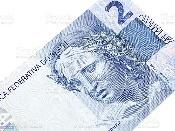
\includegraphics[width=0.79592in,height=0.59694in]{media/image47.jpg} &
TARTARUGA-MARINHA & AZUL & R\$ 2,00\tabularnewline
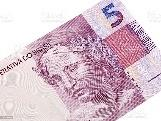
\includegraphics[width=0.73274in,height=0.54956in]{media/image48.jpg} &
GARÇA & ROSA & R\$ 5,00\tabularnewline
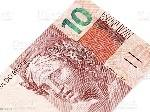
\includegraphics[width=0.68163in,height=0.51122in]{media/image49.jpg} &
ARARA VERMELHA & VERMELHA & R\$ 10,00\tabularnewline
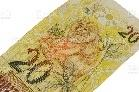
\includegraphics[width=0.63139in,height=0.41990in]{media/image50.jpg} &
MICO-LEÃO-DOURADO & AMARELA & R\$ 20,00\tabularnewline
\includegraphics[width=0.63326in,height=0.42114in]{media/image51.jpg} &
ONÇA-PINTADA & LARANJA & R\$ 50,00\tabularnewline
\includegraphics[width=0.62794in,height=0.47095in]{media/image52.jpg} &
GAROUPA & AZUL & R\$ 100,00\tabularnewline
\includegraphics[width=0.63126in,height=0.42104in]{media/image53.jpg} &
LOBO-GUARÁ & BRANCA & R\$ 200,00\tabularnewline
\bottomrule
\end{longtable}

AGORA, OBSERVE AS MOEDAS E PERCEBA SUAS DIFERENÇAS. A MOEDA DE MENOR VALOR É A DE 1 CENTAVO, QUE REPRESENTA UM REAL DIVIDIDO EM 100 PARTES. A MOEDA DE MAIOR VALOR É A DE 1 REAL, QUE EQUIVALE A CEM CENTAVOS.
}

\coment{É importante que as crianças usem as peculiaridades de
cada cédula, como a cor predominante e o animal estampado, para
identificar o valor, além do número impresso. Se possível, mostre aos alunos cédulas
verdadeiras, com o intuito de lhes mostrar a marca d'água e outras
características que apontem para sua autenticidade.}


%\textless{}https://br.freepik.com/fotos-gratis/dinheiro-moedas-brasileiras-escada\_23076933.htm\#page=9\&query=REAIS\%20moedas\&position=39\&from\_view=search\&track=ais\textgreater{}

\includegraphics[width=5.90556in,height=1.41667in]{media/image54.jpg}

\colorsec{ATIVIDADES}

\num{1} MARQUE, NA ETIQUETA, O VALOR DE CADA PRODUTO.

%\textless{}https://br.freepik.com/vetores-gratis/colecao-de-brinquedos-de-natal-desenhada-a-mao\_11105919.htm\#query=brinquedos\%20com\%20etiquetas\&position=14\&from\_view=search\&track=ais. Inserir na coluna da direita uma figura de etiqueta para o aluno preencher o valor da mercadoria.\textgreater{}

\begin{longtable}[]{@{}lll@{}}
\toprule
\includegraphics[width=1.70857in,height=2.10446in]{media/image55.png} &
Cento e trinta e cinco reais e vinte centavos. &
\includegraphics[width=2.19822in,height=2.44826in]{media/image56.png}\tabularnewline
\bottomrule
\end{longtable}

%R\$ 135,20.

\begin{longtable}[]{@{}lll@{}}
\toprule
\includegraphics[width=1.16683in,height=1.08348in]{media/image57.png} &
cinquenta e cinco reais e vinte e cinco centavos. &
\includegraphics[width=2.19822in,height=2.44826in]{media/image56.png}\tabularnewline
\bottomrule
\end{longtable}

%R\$ 55,25.

\pagebreak

\begin{longtable}[]{@{}lll@{}}
\toprule
\includegraphics[width=1.96902in,height=1.29185in]{media/image58.png} &
noventa e oito reais. &
\includegraphics[width=2.19822in,height=2.44826in]{media/image56.png}\tabularnewline
\bottomrule
\end{longtable}

%R\$ 98,00.

\begin{longtable}[]{@{}lll@{}}
\toprule
\includegraphics[width=1.60439in,height=1.38561in]{media/image59.png} &
quarenta e dois reais e noventa e nove centavos. &
\includegraphics[width=2.19822in,height=2.44826in]{media/image56.png}\tabularnewline
\bottomrule
\end{longtable}

%R\$ 42,99.

\num{2} ESCREVA POR EXTENSO OS VALORES EM REAIS.

%\textless{}Inserir a tabela conforme o modelo abaixo\textgreater{}

\begin{escolha}
\item R\$ 135,60 \reduline{Cento e trinta e cinco reais e sessenta centavos.\hfill}

\item R\$ 465,00 \reduline{Quatrocentos e sessenta e cinco reais.\hfill}

\item R\$ 59,30 \reduline{Cinquenta e nove reais e trinta centavos.\hfill}

\item R\$ 74,15 \reduline{Setenta e quatro reais e quinze centavos.\hfill}

\item R\$ 63,20 \reduline{Sessenta e três reais e vinte centavos.\hfill}

\item R\$ 15,15 \reduline{Quinze reais e quinze centavos.\hfill}
\end{escolha}

\pagebreak
\num{3} LIGUE CORRETAMENTE CADA VALOR A UMA IMAGEM.

%\textless{}https://br.freepik.com/fotos-gratis/dinheiro-moedas-brasileiras-1-real\_22809605.htm\#query=moeda\%20de\%201\%20real\%20dineiro\%20barssileiro\&position=1\&from\_view=search\&track=ais; https://br.freepik.com/fotos-gratis/dinheiro-moedas-brasileiras-5-centavos\_22781620.htm\#query=moeda\%20de\%205\%20centavos\%20dineiro\%20barssileiro\&position=2\&from\_view=search\&track=ais; https://br.freepik.com/fotos-gratis/dinheiro-moedas-brasileiras-10-centavos\_22781622.htm\#query=moeda\%20de\%2010\%20centavos\%20dineiro\%20barssileiro\&position=6\&from\_view=search\&track=ais;

\begin{multicols}{2}
R\$ 0,05 

R\$ 0,50 

R\$ 0,25 

R\$ 0,10 

R\$ 1,00 

\columnbreak


\includegraphics[width=0.80577in,height=0.79447in]{media/image60.jpg}

\includegraphics[width=0.69145in,height=0.53632in]{media/image61.jpg}

\includegraphics[width=0.75523in,height=0.67928in]{media/image62.jpg}

\includegraphics[width=0.67617in,height=0.63139in]{media/image63.jpg}

\includegraphics[width=0.69044in,height=0.66964in]{media/image64.jpg}
\end{multicols}

\coment{Se os alunos tiverem alguma dificuldade com esta atividade,
uma vez que ainda não tiveram contato com números fracionários, ajude-os
a associarem os valores às imagens das moedas.}

\num{4} PREENCHA CADA ESPAÇO COM A QUANTIDADE DE CÉDULAS NECESSÁRIAS PARA COMPRAR O ITEM CORRESPONDENTE. USE SOMENTE CÉDULAS.

%\textless{}https://www.istockphoto.com/br/foto/notas-de-dinheiro-do-brasil-em-composto-detalhes-de-notas-de-200-50-10-5-e-2-reais-gm1280319451-378658163?phrase=200\%20REAIS. Inserir quadros para que os alunos consigam colocar a quantidade de notas necessárias.\textgreater{}

\begin{escolha}
\item UM CARRINHO DE R\$ 100,00.

\includegraphics[width=.8\textwidth]{media/image65.png}

\item UMA BONECA DE R\$ 70,00.

\includegraphics[width=.8\textwidth]{media/image66.png}

\item UMA CALÇA DE R\$ 137,00.

\includegraphics[width=.8\textwidth]{media/image67.png}

\item UMA SAIA DE R\$ 85,00.

\includegraphics[width=.8\textwidth]{media/image68.png}

\item UM CHOCOLATE DE R\$ 6,00.

\includegraphics[width=.8\textwidth]{media/image69.png}

\item UM PAR DE ÓCULOS ESCUROS DE R\$ 450,00.

\includegraphics[width=.8\textwidth]{media/image70.png}
\end{escolha}

\coment{Exceto para o chocolate, de R\$ 6,00, há mais de uma combinação possível para cada item. É de suma importância
trabalhar com os alunos as respostas diferentes.}

\num{5} PREENCHA CADA CÍRCULO COM A QUANTIDADE DE MOEDAS NECESSÁRIAS PARA COMPRAR O ITEM CORRESPONDENTE. USE SOMENTE MOEDAS.

%\textless{}https://br.freepik.com/fotos-gratis/dinheiro-moedas-brasileiras-escada\_23076933.htm\#page=9\&query=REAIS\%20moedas\&position=39\&from\_view=search\&track=ais. Inserir os círculos abaixo de cada moeda para o aluno preencher a quantidade necessária.\textgreater{}

\begin{escolha}
\item UM PIRULITO DE R\$ 0,35 (TRINTA E CINCO CENTAVOS).

\includegraphics[width=.7\textwidth]{media/image71.png}

\item UMA BALA DE R\$ 0,15 (QUINZE CENTAVOS).

\includegraphics[width=.7\textwidth]{media/image72.png}

\item UM APITO DE R\$ 0,30 (TRINTA CENTAVOS).

\includegraphics[width=.7\textwidth]{media/image73.png}

\item UM CHAVEIRO DE SUPER-HERÓI DE R\$ 3,75 (TRÊS REAIS E SETENTA E CINCO

\includegraphics[width=.7\textwidth]{media/image74.png}
\end{escolha}

\coment{Os alunos precisarão de uma ajuda extra por não conhecerem números fracionários.}

\num{6} JOÃO E BIANCA GANHARAM R\$ 10,00 (CADA UM). JOÃO COMPROU UM DOCE DE R\$ 6,00,
E BIANCA COMPROU UM DOCE DE R\$ 5,00. SOBRE ESSA SITUAÇÃO, RESPONDA AO QUE SE PERGUNTA A SEGUIR.

\begin{escolha}
\item QUANTO JOÃO E BIANCA GANHARAM JUNTOS? RESPONDA COM ALGARISMOS E POR EXTENSO.

\reduline{R\$ 10,00 + R\$ 10,00 = R\$ 20,00 -- vinte reais.\hfill}

\item QUANTO JOÃO E BIANCA GASTARAM JUNTOS?

\reduline{R\$ 6,00 + R\$ 5,00 = R\$ 11,00 -- onze reais.\hfill}

\item QUANTO DINHEIRO SOBROU PARA JOÃO E BIANCA JUNTOS?

\reduline{R\$ 20,00 -- R\$ 11,00 = R\$ 9,00 -- nove reais.\hfill}

\item DESENHE, INCLUSIVE COM CORES, AS CÉDULAS E AS MOEDAS DO REAL. TENTE SE LEMBRAR DO MAIOR NÚMERO POSSÍVEL DE DETALHES DE CADA UMA.
\end{escolha}

\begin{mdframed}[linewidth=2pt,linecolor=salmao,roundcorner=10pt]
\vspace{13cm}
\end{mdframed}


\colorsec{TREINO}

\num{1} OBSERVE A IMAGEM A SEGUIR.

%\textless{}https://www.istockphoto.com/br/foto/brasileiro-dinheiro-novo-gm492494099-40521892?phrase=10\%20REAIS\textgreater{}

\begin{figure}[htpb!]
\centering
\includegraphics[width=1.92157in,height=1.43284in]{media/image75.png}
\end{figure}

O VALOR DA CÉDULA REPRESENTADA NA IMAGEM É DE


\begin{escolha}
\item R\$ 0,10.

\item R\$ 1,00.

\item R\$ 10,00.

\item R\$ 100,00.
\end{escolha}

\coment{SAEB: Relacionar valores de moedas e/ou cédulas do sistema
monetário brasileiro, com base nas imagens desses objetos.
BNCC: EF01MA19 -- Reconhecer e relacionar valores de moedas e cédulas do
sistema monetário brasileiro para resolver situações simples do
cotidiano do estudante.}

\num{2} CRISTIANO COMPROU UM CHAPÉU DE R\$ 75,00. DE QUE FORMA ELE PODE TER PAGADO POR ESSE CHAPÉU?

\begin{escolha}
\item COM DUAS CÉDULAS DE R\$ 50,00.

\item COM TRÊS CÉDULAS DE R\$ 25,00.

\item COM TRÊS CÉDULAS DE R\$ 10,00.

\item COM TRÊS CÉDULAS DE R\$ 5,00.
\end{escolha}

\coment{SAEB: Resolver problemas que envolvam moedas e/ou cédulas do
sistema monetário brasileiro.
BNCC: EF01MA19 -- Reconhecer e relacionar valores de moedas e cédulas do
sistema monetário brasileiro para resolver situações simples do
cotidiano do estudante.}



\num{3} ANA PRECISA PAGAR UMA FATURA DE R\$ 182,00. ELA ESTÁ COM UMA CÉDULA DE R\$ 100,00, UMA CÉDULA DE R\$ 50,00, UMA CÉDULA DE R\$ 20,00 E DUAS CÉDULAS DE R\$ 5,00. PODE-SE AFIRMAR QUE ANA

\begin{escolha}
\item TEM O VALOR EXATO PARA PAGAR A FATURA.

\item CONSEGUE COMPLETAR O VALOR COM UMA MOEDA SÓ.

\item PRECISA TER PELO MENOS MAIS UMA CÉDULA DE R\$ 2,00.

\item CONTINUARIA SEM O VALOR CERTO MESMO COM MAIS UMA CÉDULA DE R\$ 5,00.
\end{escolha}

\coment{SAEB: Resolver problemas que envolvam moedas e/ou cédulas do
sistema monetário brasileiro.
BNCC: EF01MA19 -- Reconhecer e relacionar valores de moedas e cédulas do
sistema monetário brasileiro para resolver situações simples do
cotidiano do estudante.}

\chapter{SERÁ QUE VAI CHOVER?}
\markboth{Módulo 6}{}

\coment{Neste módulo, vamos trabalhar a habilidade dos alunos de
perceber que alguns fatos podem ser previsíveis, e outros não. A
noção de probabilidade matemática pode ser um pouco complexa para
crianças da idade, porém, com situações do cotidiano, pode-se fazer com que elas percebam que é mais provável que isto ou aquilo aconteça.\\
Habilidade da BNCC EF01MA20.
}

\colorsec{Habilidade do SAEB:}

\begin{itemize}
\item Classificar resultados de eventos cotidianos aleatórios como ``pouco
prováveis'', ``muito prováveis'', ``certos'' ou ``impossíveis''.
\end{itemize}


\conteudo{
COMO É POSSIVEL SABER SE VAI CHOVER OU NÃO? EXISTE TODA UMA CIÊNCIA POR TRÁS DESSA PREVISÃO: A METEOROLOGIA.
NO ENTANTO, SE OLHAMOS PARA O CÉU E O VEMOS ESCURO, CRIAMOS A EXPECTATIVA DE VAI CHOVER, MESMO SEM USAR UMA CIÊNCIA MAIS PRECISA. NA METEOROLOGIA, UMA SÉRIE DE ACONTECIMENTOS
PERMITE AOS TÉCNICOS FAZER UMA PREVISÃO DO TEMPO, MAS NÓS TAMBÉM PODEMOS FAZER PREVISÕES NO DIA A DIA. PODEMOS DIZER QUE EXISTEM QUATRO POSSIBILIDADES. POR EXEMPLO:

%\textless{}Inserir um quadro conforme o modelo a seguir, utilizando as referências: https://br.freepik.com/vetores-premium/pequeno-elefante-voar-para-o-ceu\_6579577.htm\#query=elefante\%20voando\&position=9\&from\_view=search\&track=ais; https://br.freepik.com/vetores-gratis/fundo-plano-do-polo-norte-da-temporada-de-inverno\_33138109.htm\#query=neve\&position=11\&from\_view=search\&track=sph (alterar a placa colocando nela Brasil no lugar de polo norte.; https://br.freepik.com/vetores-gratis/ilustracao-de-calor-de-verao-plana-com-homem-na-cadeira\_27995494.htm\#query=ver\%C3\%A3o\%20calor\&position=0\&from\_view=search\&track=ais; https://br.freepik.com/vetores-premium/jogador-de-futebol-jogando-futebol-em-pe\_33803714.htm\#query=bola\%20jogada\%20pra\%20cima\&position=7\&from\_view=search\&track=ais.\textgreater{}
%\begin{longtable}[]{@{}llll@{}}
%\toprule
%impossível & quando não existe a menor chance de algo acontecer & um
%elefante sair voando por conta própria &
%\includegraphics[width=1.42708in,height=1.42708in]{media/image76.jpg}\tabularnewline
%pouco provável & quando existe uma pequena chance de algo acontecer &
%nevar no brasil &
%\includegraphics[width=1.52602in,height=1.01167in]{media/image77.png}\tabularnewline
%muito provável & quando existe uma grande chance de algo acontecer &
%fazer calor no verão &
%\includegraphics[width=1.30208in,height=1.30208in]{media/image78.jpg}\tabularnewline
%certeza & quando é certo que algo vai acontecer & uma bola cair quando
%for jogada para cima &
%\includegraphics[width=1.04437in,height=1.39696in]{media/image79.jpg}\tabularnewline
%\bottomrule
%\end{longtable}
}

\coment{É importante ressaltar com os alunos que, no Brasil, é raro
nevar, mas pode acontecer, principalmente na região Sul. Vale
ressaltar também que nem todos os dias do verão são quentes, ou seja, a
temperatura pode cair em alguns dias.}

\colorsec{ATIVIDADES}

\num{1} PINTE OS CÍRCULOS COM AS SITUAÇÕES IMPOSSÍVEIS NO QUADRO A SEGUIR. PINTE
DA COR QUE VOCÊ PREFERIR.

%\textless{}criar um quadro com as situações descritas conforme o modelo a seguir.\textgreater{} \includegraphics[width=5.16074in,height=7.09420in]{media/image80.png}

\coment{Esta atividade pode ser importante para trabalhar a
habilidade de leitura dos alunos. As situações impossíveis são: céu
ficando verde, tesoura falando, jacaré voando, leão miando, unicórnios existindo,
chuva caindo para cima e árvore andando.}

\num{2} NOS QUADROS A SEGUIR, DESENHE DUAS SITUAÇÕES QUE VOCÊ CONSIDERE
IMPOSSÍVEIS. NÃO REPITA AS SITUAÇÕES DA ATIVIDADE ANTERIOR CONSIDERADAS IMPOSSÍVEIS.

%\textless{}Inserir dois quadros para os alunos desenharem, tomando toda a página\textgreater{} \includegraphics[width=4.38938in,height=7.65199in]{media/image81.png}

\coment{Permita que os alunos utilizem a
imaginação sem moderação. Começar com os acontecimentos
impossíveis é importante, pois permite que o aluno utilize sua
imaginação, provocando engajamento e envolvimento na criança.}

\num{3} LIGUE CADA SITUAÇÃO COM A IMAGEM CORRESPONDENTE.

%\textless{}https://br.freepik.com/vetores-gratis/chovendo-na-natureza-paisagem\_5769787.htm\#query=rel\%C3\%A3mpago\%20na\%20chuva\&position=6\&from\_view=search\&track=ais; https://br.freepik.com/vetores-gratis/tartaruga-jogando-skate-no-parque\_4119896.htm\#query=sapo\%20jogando\%20volei\&position=0\&from\_view=search\&track=ais;

%\begin{longtable}[]{@{}ll@{}}
%\toprule
%\begin{minipage}[t]{0.48\columnwidth}\raggedright\strut
%\includegraphics[width=2.03487in,height=1.82023in]{media/image82.jpg}
%
%relampejar na chuva\strut
%\end{minipage} & \begin{minipage}[t]{0.48\columnwidth}\raggedright\strut
%impossível\strut
%\end{minipage}\tabularnewline
%\begin{minipage}[t]{0.48\columnwidth}\raggedright\strut
%\includegraphics[width=2.11035in,height=1.45968in]{media/image83.jpg}
%
%tartaruga \textit{skatista}\strut
%\end{minipage} & \begin{minipage}[t]{0.48\columnwidth}\raggedright\strut
%pouco provável\strut
%\end{minipage}\tabularnewline
%\begin{minipage}[t]{0.48\columnwidth}\raggedright\strut
%\includegraphics[width=2.11129in,height=1.37616in]{media/image84.jpg}
%
%acidente aéreo\strut
%\end{minipage} & \begin{minipage}[t]{0.48\columnwidth}\raggedright\strut
%muito provável\strut
%\end{minipage}\tabularnewline
%\begin{minipage}[t]{0.48\columnwidth}\raggedright\strut
%\includegraphics[width=1.86458in,height=1.86458in]{media/image85.jpg}
%
%sentir fome\strut
%\end{minipage} & \begin{minipage}[t]{0.48\columnwidth}\raggedright\strut
%certo\strut
%\end{minipage}\tabularnewline
%\bottomrule
%\end{longtable}

\num{4} PREENCHA COM UM X AS POSSIBILIDADES DO QUADRO A SEGUIR.

\begin{longtable}[]{@{}lllll@{}}
\toprule
situação & impossível & pouco provável & muito provável &
certa\tabularnewline
esquecer-se de escovar os dentes & & & &\tabularnewline
esquecer-se de fazer a lição & & & &\tabularnewline
jogar \textit{videogame} todo o dia & & & &\tabularnewline
sentir vontade de ir ao banheiro & & & &\tabularnewline
brincar com um adulto & & & &\tabularnewline
brincar com outra criança & & & &\tabularnewline
receber um amigo em casa & & & &\tabularnewline
esquecer a luz acesa & & & &\tabularnewline
esquecer-se de dar a descarga depois de usar o banheiro & & &
&\tabularnewline
comer doces fora de hora & & & &\tabularnewline
assitir à tv ou ficar na internet na hora de comer & & & &\tabularnewline
\bottomrule
\end{longtable}

\coment{Com esta atividade, pode-se auxiliar o aluno a fazer uma autoavaliação de como ele administra seu tempo diariamente, além de ajudá-lo
a criar suas prioridades. A atividade favorece o trabalho com os temas contemporâneos transversair sáude e vida familiar e social.}

\num{5} ZÉLIA ESTAVA BRINCANDO DE JOGAR UM DADO. NO QUADRO A SEGUIR, PINTE QUAIS SÃO
OS RESULTADOS PROVÁVEIS DE SAÍREM QUANDO ZÉLIA JOGAR UMA VEZ.

\begin{longtable}[]{@{}llll@{}}
\toprule
%\includegraphics[width=1.55208in,height=1.55208in]{media/image86.jpg} &
1 & 15 & 6\tabularnewline
& 20 & 3 & 8\tabularnewline
& 5 & 10 & 9\tabularnewline
& 11 & 4 & 12\tabularnewline
& 13 & 14 & 2\tabularnewline
\bottomrule
\end{longtable}

\coment{Espera-se que os alunos percebram que só podem sair os
resultados de 1 a 6, visto que são os únicos números que há em um
dado. Se possível, mostre um dado para os alunos durante a
atividade.}

\num{6} DESCUBRA QUAL DOS JOGADORES A SEGUIR TEM A MAIOR CHANCE DE GANHAR O JOGO
DE DOMINÓS. CIRCULE O NOME DESSE JOGADOR.

%\textless{}https://br.freepik.com/vetores-gratis/ilustracao-realista-de-jogo-de-domino\_22656073.htm\#query=domin\%C3\%B3\%20jogada\&position=29\&from\_view=search\&track=ais; https://br.freepik.com/vetores-premium/stock-vector-domino-conjunto-completo-ilustracao-realista-colecao-de-cartoes-de-domino-de-cor-preto-e-branco\_22221437.htm\#query=domin\%C3\%B3\%20jogada\&position=35\&from\_view=search\&track=ais\textgreater{} \includegraphics[width=4.84499in,height=2.71476in]{media/image87.png}

\coment{Solange é a única
jogadora que possui uma pedra com o número 5. Nenhum outro jogador
possui uma pedra assim; logo a chance de vitória de Solange é maior.}

\num{7} BERNARDO ESTÁ BRINCANDO DE COLOCAR DIFERENTES TIPOS DE BOLA NA ÁGUA
PARA VER QUAL FLUTUA. VOCÊ CONSEGUE PREVER QUAL SERÁ O RESULTADO? ASSINALE
COM UM X.

%\textless{}Inserir quadro conforme o modelo a seguir, utilizando as referências: https://br.freepik.com/fotos-premium/bola-de-papel-amassado\_25578632.htm?query=bola\%20de\%20papel\#from\_view=detail\_alsolike https://br.freepik.com/vetores-premium/bola-de-cromo-3d-realista-isolada-no-fundo-branco\_34098681.htm\#query=bola\%20de\%20metal\&position=24\&from\_view=search\&track=ais; https://br.freepik.com/vetores-premium/esfera-branca-bola-ilustracao\_9402860.htm\#query=bola\%20de\%20isopor\&position=13\&from\_view=search\&track=ais; https://br.freepik.com/vetores-premium/bola-de-bilhar\_26468289.htm\#query=bola\%20de\%20bilhar\&position=46\&from\_view=search\&track=ais \textgreater{}

%\begin{longtable}[]{@{}llll@{}}
%\toprule
%\begin{minipage}[t]{0.24\columnwidth}\raggedright\strut
%\includegraphics[width=1.06165in,height=0.99037in]{media/image88.jpg}
%
%Bola de papel flutua?\strut
%\end{minipage} & \begin{minipage}[t]{0.24\columnwidth}\raggedright\strut
%\includegraphics[width=0.98125in,height=0.98125in]{media/image89.jpg}
%
%Bola de metal flutua?\strut
%\end{minipage} & \begin{minipage}[t]{0.24\columnwidth}\raggedright\strut
%\includegraphics[width=0.83333in,height=0.83333in]{media/image90.jpg}
%
%Bola de isopor flutua?\strut
%\end{minipage} & \begin{minipage}[t]{0.24\columnwidth}\raggedright\strut
%\includegraphics[width=0.83333in,height=0.83333in]{media/image91.jpg}
%
%Bola de bilhar flutua?\strut
%\end{minipage}\tabularnewline
%sim & & sim &\tabularnewline
%não & & não &\tabularnewline
%talvez & & talvez &\tabularnewline
%\bottomrule
%\end{longtable}

\coment{Ainda que os alunos não conheçam o
conceito de flutuabilidade, é importante
desenvolver suas habilidades de prever um acontecimento, baseando-se no
senso comum ou até em experiências pessoais. Alguns alunos podem ter
manipulado algumas dessas bolas ou feito alguma experiência
desse tipo. Se julgar necessário, se for possível, faça a experiência em
sala de aula. Você pode promover um jogo de adivinhação, promovendo
maior engajamento dos alunos. Não é viável entrar no conceito de
densidade por ser um assunto muito complexo para a idade, porém deve-se
tomar cuidado para não criar um subsunçor na estrutura cognitiva do
aluno acerca da massa das bolas como se fosse o fator determinante para a
flutuação.}

\num{8} DISCUTA UMA SITUAÇÃO COM OS COLEGAS QUE SEJA MUITO PROVÁVEL E DESENHE
ESSA SITUAÇÃO NO QUADRO A SEGUIR. DEPOIS, DESCREVA QUE SITUAÇÃO É ESSA.

%\textless{}Inserir um quadro para o aluno desenhar além de seis linhas para o aluno descrever a situação. Essa atividade deve preencher uma página\textgreater{} \includegraphics[width=3.24914in,height=2.92171in]{media/image92.png}

\coment{Aproveite a atividade para desenvolver a habilidade de
escrita. Oriente os alunos quanto à escolha da situação.}

\num{9} DISCUTA UMA SITUAÇÃO COM OS COLEGAS QUE SEJA POUCO PROVÁVEL E DESENHE
ESSA SITUAÇÃO NO QUADRO A SEGUIR. DEPOIS, DESCREVA QUE SITUAÇÃO É ESSA.

%\textless{}Inserir um quadro para o aluno desenhar além de seis linhas para o aluno descrever a situação. Essa atividade deve preencher uma página\textgreater{} \includegraphics[width=2.86272in,height=2.57423in]{media/image92.png}


\num{10} DISCUTA UMA SITUAÇÃO COM OS COLEGAS QUE SEJA CERTA (OU SEJA, QUE REPRESENTE UMA CERTEZA) E DESENHE ESSA SITUAÇÃO NO QUADRO A SEGUIR, DEPOIS, DESCREVA QUE SITUAÇÃO É ESSA.

%\textless{}Inserir um quadro para o aluno desenhar além de seis linhas para o aluno descrever a situação. Essa atividade deve preencher uma página\textgreater{} \includegraphics[width=2.86272in,height=2.57423in]{media/image92.png}

\colorsec{TREINO}

\num{1} UMA SITUAÇÃO IMPOSSÍVEL DE ACONTECER É

\begin{escolha}
\item UMA CANETA ESCREVER.

\item UM GATO DORMIR.

\item UM NAVIO FLUTUAR.

\item UM PEIXE CANTAR.
\end{escolha}

\coment{SAEB: Classificar resultados de eventos cotidianos aleatórios como
``pouco prováveis'', ``muito prováveis'', ``certos'' ou ``impossíveis''.
BNCC: EF01MA20 -- Classificar eventos envolvendo o acaso, tais como
``acontecerá com certeza'', ``talvez aconteça'' e ``é impossível
acontecer'', em situações do cotidiano.}

\num{02} INDIQUE QUAL DESTAS SITUAÇÕES É POUCO PROVÁVEL DE ACONTECER.

\begin{escolha}
\item FAZER CALOR NO VERÃO.

\item FAZER FRIO NO VERÃO.

\item NEVAR NO INVERNO.

\item SURGIREM FLORES NA PRIMAVERA.
\end{escolha}

\coment{SAEB: Classificar resultados de eventos cotidianos aleatórios como
``pouco prováveis'', ``muito prováveis'', ``certos'' ou ``impossíveis''.
BNCC: EF01MA20 -- Classificar eventos envolvendo o acaso, tais como
``acontecerá com certeza'', ``talvez aconteça'' e ``é impossível
acontecer'', em situações do cotidiano.}



\num{3} ANALISE ESTA IMAGEM.

%Inserir imagem: https://br.freepik.com/fotos-gratis/bela-vista-de-uma-estrada-vazia-cercada-por-vegetacao-sob-nuvens-escuras-de-tempestade_17110244.htm#query=tempo%20nublado&position=1&from_view=search&track=ais

O QUE SE PODE AFIRMAR SOBRE A POSSIBILIDADE DE CHUVA NA REGIÃO RETRATADA NA IMAGEM?

\begin{escolha}
\item É IMPOSSÍVEL QUE CHOVA.

\item É CERTO QUE CHOVA.

\item É POUCO PROVÁVEL QUE CHOVA.

\item É MUITO PROVÁVEL QUE CHOVA.
\end{escolha}

\coment{SAEB: Classificar
resultados de eventos cotidianos aleatórios como ``pouco prováveis'',
``muito prováveis'', ``certos'' ou ``impossíveis''.
BNCC: EF01MA20 -- Classificar eventos envolvendo o acaso, tais como
``acontecerá com certeza'', ``talvez aconteça'' e ``é impossível
acontecer'', em situações do cotidiano.}

\chapter{TUDO ORGANIZADINHO}
\markboth{Módulo 7}{}

\coment{Neste módulo, vamos desenvolver nos alunos a habilidade de identificar e
colocar informações em gráficos e tabelas.\\
Habilidades da BNCC EF01MA21, EF01MA22.}

\colorsec{Habilidades do SAEB:}

\begin{itemize}
\item Ler/identificar ou comparar dados estatísticos ou informações,
expressos em tabelas (simples ou de dupla entrada).

\item Ler/identificar ou comparar dados estatísticos expressos em gráficos
(barras simples, colunas simples ou pictóricos).

\item Representar os dados de uma pesquisa estatística ou de um levantamento
em listas, tabelas (simples ou de dupla entrada) ou gráficos (barras
simples, colunas simples ou pictóricos).
\end{itemize}


\conteudo{
VOCÊ JÁ PERCEBEU COMO LISTAS
DE COMPRAS, LISTAS DE MATERIAIS DA ESCOLA OU ENTÃO O
\emph{RANKING} DE UM JOGO FICAM ORGANIZADOS? ELES FICAM ORGANIZADOS EM ESTRUTURAS QUE CHAMAMOS DE \textbf{TABELA}. OBSERVE:

%\textless{}Inserir a referência: https://br.freepik.com/vetores-gratis/tabela-de-classificacao-com-fundo-abstrato\_11187227.htm\#query=score\%20game\&position=0\&from\_view=search\&track=ais. Não é necessário traduzir. Os alunos estão habituados a \emph{games} e suas terminologias nessa idade.\textgreater{}

%\includegraphics[width=1.77083in,height=1.77083in]{media/image93.jpg}

a CLASSIFICAÇÃO E OS PONTOS DOS JOGADORES DESSE JOGO SÃO APRESENTADOS EM
UMA TABELA. COMO TEMOS DUAS INFORMAÇÕES, OU SEJA, A CLASSIFICAÇÃO E A
PONTUAÇÃO, DIZEMOS QUE SE TRATA DE UMA \textbf{TABELA DE DUPLA ENTRADA}.

OUTRO MODO DE ORGANIZAR INFORMAÇÕES SÃO OS \textbf{GRÁFICOS}. VEJA:

%\textless{}Criar gráficos conforme o modelo a seguir.\textgreater{}
%{{[}CHART{]}}\includegraphics[width=3.13415in,height=1.79094in]{media/image94.png}

EM UMA ESCOLA, PERGUNTARAM PARA QUE TIME OS ALUNOS DE UMA TURMA TORCIAM. O
RESULTADO ESTÁ NESSES GRÁFICOS. PERCEBA QUE A MAIORIA DAS CRIANÇAS
TORCIA PARA O SABÁTICO. OS GRÁFICOS AJUDAM A PERCEBER ISSO MAIS FACILMENTE. VOCÊ SABERIA DIZER, SÓ OLHANDO PARA ELES, QUAL TIME FOI O MENOS ESCOLHIDO?
}

\colorsec{ATIVIDADES}

\num{1} ANALISE A TABELA, QUE MOSTRA A PONTUAÇÃO DE JOGADORES EM UMA PARTIDA DE
BOLICHE.

%\textless{}Inserir tabela conforme o modelo a seguir. Inserir a referência: https://br.freepik.com/vetores-premium/jogador-de-boliche\_2938032.htm\#query=boliche\%20crian\%C3\%A7as\&position=5\&from\_view=search\&track=ais.\textgreater{} \includegraphics[width=1.88542in,height=1.88542in]{media/image95.jpg}

\begin{longtable}[]{@{}ll@{}}
\toprule
jogador & pontuação\tabularnewline
\midrule
\endhead
marcos & 46\tabularnewline
ricardo & 56\tabularnewline
suzana & 32\tabularnewline
hévilin & 31\tabularnewline
débora & 47\tabularnewline
lucas & 35\tabularnewline
marcelo & 35\tabularnewline
\bottomrule
\end{longtable}

AGORA, RESPONDA AO QUE SE PERGUNTA A SEGUIR.

\begin{escolha}
\item QUEM FEZ MAIS PONTOS?

\reduline{Ricardo tem a maior pontuação.\hfill}

\item QUEM FEZ MENOS PONTOS?

\reduline{Hévilin tem a menor pontuação.\hfill}

\item HOUVE ALGUM EMPATE?

\reduline{Lucas e Marcelo empataram com 35 pontos.\hfill}

\item QUEM SÃO OS TRÊS PRIMEIROS COLADOS AO FINAL DA PARTIDA?

\reduline{Ricardo (1º), Débora (2º) e Marcos (3º).\hfill}
\end{escolha}

\num{02} EM UMA TURMA DE PRIMEIRO ANO, FOI FEITA UMA PESQUISA PARA SABER QUE TIPO DE ALIMENTO AS
CRIANÇAS MAIS COMIAM. O RESULTADO ESTÁ REPRESENTADO NO GRÁFICO A SEGUIR. ANALISE-O.

%\textless{}Inserir gráfico conforme o modelo a seguir.\textgreater{}
%%{{[}CHART{]}}

Agora, responda ao que se pergunta a seguir?

\begin{escolha}
\item QUAL É A COMIDA PREFERIDA DESSA TURMA?

\reduline{A maioria dos alunos prefere massa.\hfill}

\item QUAL É A COMIDA MENOS QUERIDA DESSA TURMA?

\reduline{A minoria dos alunos costuma comer verduras.\hfill}

\item QUAL É A SEGUNDA COMIDA PREFERIDA DOS ALUNOS DESSA TURMA?

\reduline{Doces são a segunda comida preferida dos alunos.\hfill}

\item QUAL DAS COMIDAS VOCÊ TERIA ESCOLHIDO COMO A SUA FAVORITA? POR QUÊ?

\reduline{Resposta pessoal.\hfill}
\linhas{2}
\end{escolha}

\num{3} A TABELA A SEGUIR MOSTRA A LISTA DOS JOGOS MAIS JOGADOS E MAIS CURTIDOS PELOS
ALUNOS DE UMA TURMA DE PRIMEIRO ANO. A TABELA TAMBÉM MOSTRA QUANTOS ALUNOS PREFEREM CADA
JOGO.

\begin{longtable}[]{@{}ll@{}}
\toprule
\emph{minecraft} & 8\tabularnewline
\emph{mario kart 8} & 9\tabularnewline
\emph{animal crossing: new horizons} & 5\tabularnewline
\emph{super mario party} & 3\tabularnewline
\emph{roblox} & 10\tabularnewline
\bottomrule
\end{longtable}

\begin{escolha}
\item NA TABELA A SEGUIR, COLOQUE OS JOGOS EM ORDEM DO MAIS JOGADO PARA O MENOS JOGADO.

\begin{longtable}[]{@{}ll@{}}
\toprule
\emph{minecraft} & 3\tabularnewline
\emph{mario kart 8} & 2\tabularnewline
\emph{animal crossing: new horizons} & 4\tabularnewline
\emph{super mario party} & 5\tabularnewline
\emph{roblox} & 1\tabularnewline
\bottomrule
\end{longtable}

\item PREENCHA O GRÁFICO A SEGUIR, PINTANDO OS QUADRADINHOS CONFORME A TABELA DE ALUNOS.

\begin{longtable}[]{@{}llllll@{}}
\toprule
10 & & & & &\tabularnewline
9 & & & & &\tabularnewline
8 & & & & &\tabularnewline
7 & & & & &\tabularnewline
6 & & & & &\tabularnewline
5 & & & & &\tabularnewline
4 & & & & &\tabularnewline
3 & & & & &\tabularnewline
2 & & & & &\tabularnewline
1 & & & & &\tabularnewline
jogos & \emph{minecraft} & \emph{mario kart 8} & \emph{animal crossing:
new horizons} & \emph{super mario party} & \emph{roblox}\tabularnewline
\bottomrule
\end{longtable}

\end{escolha}

\coment{Oriente os alunos a transferirem as informações da
primeira tabela para o gráfico de barras. Explique aos alunos que cada
quadradinho é um aluno que escolheu o jogo selecionado. Esta atividade
favorece o trabalho com a competência geral 5 da BNCC.}

\num{4} VAMOS BRINCAR DE JOGAR DADO? PEGUE UM DADO DE 6 LADOS E LANCE-O DEZ
VEZES. PINTE A QUANTIDADE DE QUADRADINHOS DE CADA JOGADA NO GRÁFICO
A SEGUIR.

%\textless{}inserir a referência: https://br.freepik.com/vetores-gratis/ilustracao-de-desenho-de-tatuagem\_33488420.htm\#query=dice\%20kids\&position=4\&from\_view=search\&track=ais.\textgreater{} \includegraphics[width=1.31250in,height=1.31250in]{media/image97.jpg}

%\begin{longtable}[]{@{}lllllllllll@{}}
%\toprule
%6 \includegraphics[width=0.56258in,height=0.57300in]{media/image98.png}
%& & & & & & & & & &\tabularnewline
%5 \includegraphics[width=0.53132in,height=0.55216in]{media/image99.png}
%& & & & & & & & & &\tabularnewline
%4 \includegraphics[width=0.61467in,height=0.53132in]{media/image100.png}
%& & & & & & & & & &\tabularnewline
%3 \includegraphics[width=0.56258in,height=0.53132in]{media/image101.png}
%& & & & & & & & & &\tabularnewline
%2 \includegraphics[width=0.57300in,height=0.54174in]{media/image102.png}
%& & & & & & & & & &\tabularnewline
%1 \includegraphics[width=0.58341in,height=0.55216in]{media/image103.png}
%& & & & & & & & & &\tabularnewline
%lançamentos & 1º & 2º & 3º & 4º & 5º & 6º & 7º & 8º & 9º &
%10º\tabularnewline
%\bottomrule
%\end{longtable}

\coment{Distribua dados para os alunos ou projete um dado
\textit{on-line}. Nesta atividade, podem-se trabalhar questões como
aleatoriedade ou probabilidade, conforme módulo anterior.}

\num{5} VAMOS ENTENDER O QUE É DIVERSIDADE? VAMOS FAZER UMA PESQUISA NA TURMA E
DEPOIS PREENCHER A TABELA A SEGUIR. A PERGUNTA É: QUAL É A SUA ETNIA?

\begin{longtable}[]{@{}ll@{}}
\toprule
etnia & quantidade de alunos\tabularnewline
\midrule
\endhead
branca &\tabularnewline
preta &\tabularnewline
parda &\tabularnewline
amarela &\tabularnewline
indígena &\tabularnewline
\bottomrule
\end{longtable}

\coment{É de suma importância que esta atividade seja utilizada para trabalhar com estes temas contemporâneos transversais: diversidade cultural; educação para a valorização das
multiculturalidades nas matrizes históricas e culturais brasileiras.}

\num{6} AGORA, DESENHE UM GRÁFICO DE BARRAS COM OS DADOS DA TABELA.

\begin{longtable}[]{@{}llllll@{}}
\toprule
7 & & & & &\tabularnewline
6 & & & & &\tabularnewline
5 & & & & &\tabularnewline
4 & & & & &\tabularnewline
3 & & & & &\tabularnewline
2 & & & & &\tabularnewline
1 & & & & &\tabularnewline
& branca & preta & parda & amarela & indígena\tabularnewline
\bottomrule
\end{longtable}

\coment{Oriente os alunos a preencherem o gráfico desenhando
barras que tenham a altura correspondente ao número de alunos em cada resposta.
Se a sala tiver mais alunos, oriente-os a montarem o gráfico no caderno.}

\num{7} NA TABELA A SEGUIR, MOSTRAM-SE AS TEMPERATURAS NA CIDADE DE SÃO PAULO EM CINCO
DIAS QUAISQUER.

%\textless{}Inserir a referência: https://br.freepik.com/vetores-gratis/contraste-de-inverno-e-verao-clima-frio-e-quente\_18733427.htm\#query=temperatura\&position=26\&from\_view=search\&track=sph.\textgreater{}\includegraphics[width=2.20878in,height=1.47139in]{media/image104.jpg}

\begin{longtable}[]{@{}lllll@{}}
\toprule
Segunda-feira & Terça-feira & Quarta-feira & Quinta-feira & Sexta-feira\tabularnewline
\midrule
\endhead
37° & 35° & 22° & 20° & 19°\tabularnewline
\bottomrule
\end{longtable}

AGORA, RESPONDA AO QUE SE PERGUNTA A SEGUIR.

\begin{escolha}
\item QUAL FOI O DIA MAIS QUENTE DESSA SEMANA?

\reduline{Foi a segunda-feira.\hfill}

\item QUAL FOI O DIA MAIS FRIO DESSA SEMANA?

\reduline{Foi a sexta-feira.\hfill}

\item AO LONGO DA SEMANA, A TEMPERATURA ESTÁ AUMENTANDO OU DIMINUINDO?

\reduline{Espera-se que os alunos percebam que os valores das temperaturas diminuíram ao longo da semana.\hfill}

\item DESENHE AS BARRAS DE UM GRÁFICO COM OS DADOS DA TABELA.

\begin{longtable}[]{@{}llllll@{}}
\toprule
40 & & & & &\tabularnewline
30 & & & & &\tabularnewline
20 & & & & &\tabularnewline
10 & & & & &\tabularnewline
0 & & & & &\tabularnewline
& Segunda-feira & Terça-feira & Quarta-feira & Quinta-feira & Sexta-feira\tabularnewline
\bottomrule
\end{longtable}

\end{escolha}

\coment{Faça os alunos perceberem que, da esquerda para a direita, as barras têm
tamanhos decrescentes, em virtude de as temperaturas estarem diminuindo
ao logo da semana.}

\num{8} PINTE OS TROFÉUS DO GRÁFICO CONFORME A QUANTIDADE DE TÍTULOS DA COPA DO
MUNDO DA FIFA DE CADA SELEÇÃO. CONFIRA A TABELA.

\begin{longtable}[]{@{}ll@{}}
\toprule
seleção & vitórias em copas do mundo da fifa\tabularnewline
\midrule
\endhead
brasil & 5\tabularnewline
alemanha & 4\tabularnewline
itália & 4\tabularnewline
argentina & 3\tabularnewline
frança & 2\tabularnewline
uruguai & 2\tabularnewline
espanha & 1\tabularnewline
inglaterra & 1\tabularnewline
\bottomrule
\end{longtable}

%\textless{}Inserir um pictograma com as taças da copa para os aluinos colorir na coluna da direita, conforme o modelo a seguir.\textgreater{}

%\begin{longtable}[]{@{}ll@{}}
%\toprule
%brasil &
%\includegraphics[width=3.05575in,height=0.58176in]{media/image105.png}\tabularnewline
%alemanha &
%\includegraphics[width=3.05575in,height=0.58176in]{media/image105.png}\tabularnewline
%itália &
%\includegraphics[width=3.05575in,height=0.58176in]{media/image105.png}\tabularnewline
%argentina &
%\includegraphics[width=3.05575in,height=0.58176in]{media/image105.png}\tabularnewline
%frança &
%\includegraphics[width=3.05575in,height=0.58176in]{media/image105.png}\tabularnewline
%uruguai &
%\includegraphics[width=3.05575in,height=0.58176in]{media/image105.png}\tabularnewline
%espanha &
%\includegraphics[width=3.05575in,height=0.58176in]{media/image105.png}\tabularnewline
%inglaterra &
%\includegraphics[width=3.05575in,height=0.58176in]{media/image105.png}\tabularnewline
%\bottomrule
%\end{longtable}

\colorsec{TREINO}

\num{1} ANALISE O GRÁFICO, QUE MOSTRA A PREFERÊNCIA DE FRUTAS DOS ALUNOS DO PRIMEIRO ANO.

%{{[}CHART{]}}

A fruta mais escolhida é

\begin{escolha}
\item A BANANA.

\item A MAÇÃ.

\item O MORANGO.

\item A PERA.
\end{escolha}

\coment{SAEB: Ler/identificar ou comparar dados estatísticos expressos
em gráficos (barras simples, colunas simples ou pictóricos).
BNCC: EF01MA21 -- Ler dados expressos em tabelas e em gráficos de colunas
simples.}

\num{2} ANALISE A TABELA, QUE FORNECE INFORMAÇÕES SOBRE OS ALUNOS DE UMA ESCOLA QUE OUVEM DETERMINADOS ESTILOS MUSICAIS.

\begin{longtable}[]{@{}ll@{}}
\toprule
estilo musical & número de alunos que ouvem\tabularnewline
\midrule
\endhead
pagode & 2\tabularnewline
rock & 2\tabularnewline
sertanejo & 6\tabularnewline
funk & 2\tabularnewline
clássica & 1\tabularnewline
\bottomrule
\end{longtable}

QUAL É ESTILO DE MÚSICA MENOS OUVIDO PELOS ALUNOS DA ESCOLA?

\begin{escolha}
\item CLÁSSICA.

\item FUNK.

\item ROCK.

\item SERTANEJO.
\end{escolha}

\coment{SAEB: Ler/identificar ou comparar dados estatísticos ou informações, expressos
em tabelas (simples ou de dupla entrada).
BNCC: EF01MA21 -- Ler dados expressos em tabelas e em gráficos de colunas
simples.}


\num{3} ANALISE O GRÁFICO A SEGUIR, QUE DEMONSTRA ESPORTES ESCOLHIDOS POR ALGUNS ALUNOS.

%{{[}CHART{]}}

INDIQUE QUAL É O ESPORTE MENOS ESCOLHIDO PELOS ALUNOS.

\begin{escolha}
\item BASQUETE.

\item FUTEBOL.

\item JUDÔ.

\item TÊNIS DE MESA.
\end{escolha}

\coment{SAEB:
Ler/identificar ou comparar dados estatísticos expressos em gráficos
(barras simples, colunas simples ou pictóricos).
BNCC: EF01MA21 -- Ler dados expressos em tabelas e em gráficos de colunas
simples.}

\chapter{SIMULADO 1}
\markboth{Simulado 1}{}

\num{1} NO PACOTE DE AÇÚCAR QUE COMPRAMOS NO SUPERMERCADO, GERALMENTE HÁ UM NÚMERO
1 SEGUIDO DA UNIDADE ``KG''. O QUE ESSE NÚMERO REPRESENTA?

\begin{escolha}
\item CÓDIGO DE IDENTIFICAÇÃO.

\item MEDIDA.

\item QUANTIDADE.

\item ORDEM.
\end{escolha}

\coment{SAEB: Reconhecer o que os números naturais indicam em diferentes
situações: quantidade, ordem, medida ou código de identificação.
BNCC: EF01MA01 -- Utilizar números naturais como indicador de quantidade
ou de ordem em diferentes situações cotidianas e reconhecer situações em
que os números não indicam contagem nem ordem, mas sim código de
identificação.}



\num{2} ANALISE O ALFABETO.

%\textless{}https://br.freepik.com/vetores-gratis/fontes-alfabeto-inglesas-em-cores-diferentes\_1372652.htm\#query=alfabeto\&position=1\&from\_view=search\&track=sph\textgreater{}

%\includegraphics[width=2.61848in,height=1.85732in]{media/image106.jpg}

INDIQUE QUAL É A POSIÇÃO DA LETRA G.

\begin{escolha}
\item 5 (QUINTA LETRA).

\item 6 (SEXTA LETRA).

\item 7 (SÉTIMA LETRA).

\item 8 (OITAVA LETRA).
\end{escolha}

\coment{SAEB: Identificar a posição ordinal de um objeto ou termo em uma
sequência (1º, 2º etc.)
BNCC: EF01MA01 -- Utilizar números naturais como indicador de quantidade
ou de ordem em diferentes situações cotidianas e reconhecer situações em
que os números não indicam contagem nem ordem, mas sim código de
identificação.}



\num{3}COBSERVE A SOMA.

64 + 46

O RESULTADO É

\begin{escolha}
\item 18.

\item 100.

\item 101.

\item 110.
\end{escolha}

\coment{SAEB: Calcular o resultado de adições e subtrações, envolvendo
número naturais de até 3 ordens.
BNCC: EF01MA08 -- Resolver e elaborar problemas de adição e de subtração,
envolvendo números de até dois algarismos, com os significados de
juntar, acrescentar, separar e retirar, com o suporte de imagens e/ou
material manipulável, utilizando estratégias e formas de registro
pessoais.}

\num{4} INDIQUE UMA FORMA CORRETA DE COMPOR O NÚMERO 50.

\begin{escolha}
\item 25 + 26.

\item 35 + 25.

\item 98 -- 48.

\item 100 -- 45.
\end{escolha}

\coment{SAEB: Compor ou decompor números naturais de até 3 ordens por
meio de diferentes adições.
BNCC: EF01MA07 -- Compor e decompor número de até duas ordens, por meio
de diferentes adições, com o suporte de material manipulável,
contribuindo para a compreensão de características do sistema de
numeração decimal e o desenvolvimento de estratégias de cálculo.}

\num{5} ANALISE A IMAGEM.

%\textless{}Criar uma figura com dois lápis, conforme o modelo a seguir. Utilize a referência: https://br.freepik.com/vetores-premium/icone-de-lapis-em-estilo-simples-ilustracao-vetorial-de-equipamentos-de-educacao-em-fundo-isolado-conceito-de-negocio-de-sinal-de-ferramenta-de-desenho\_30026502.htm\#query=lapis\&position=6\&from\_view=search\&track=sph.\textgreater{} \includegraphics[width=3.74118in,height=0.57310in]{media/image29.jpg}\includegraphics[width=4.71287in,height=0.53673in]{media/image29.jpg}

SOBRE OS DOIS LÁPIS DA IMAGEM, PODE-SE DIZER QUE

\begin{escolha}
\item ELES TÊM O MESMO COMPRIMENTO.

\item O LÁPIS DE BAIXO TEM MENOR COMPRIMENTO.

\item O LÁPIS DE CIMA TEM MENOR COMPRIMENTO.

\item OS COMPRIMENTOS DELES NÃO PODEM SER COMPARADOS.
\end{escolha}

\coment{SAEB: Comparar comprimentos, capacidades ou massas ou ordenar
imagens de objetos com base na comparação visual de seus comprimentos,
capacidades ou massas.
BNCC: EF01MA15 -- Comparar comprimentos, capacidades ou massas,
utilizando termos como mais alto, mais baixo, mais comprido, mais curto,
mais grosso, mais fino, mais largo, mais pesado, mais leve, cabe mais,
cabe menos, entre outros, para ordenar objetos de uso cotidiano.}

\num{6} OBSERVE A IMAGEM.

%\textless{} https://br.freepik.com/vetores-gratis/adesivo-de-copo-de-medicao-em-fundo-branco\_18180135.htm\#query=COPO\%20MEDIDORDESENHO\&position=2\&from\_view=search\&track=ais. Colocar as quantidades conforme o modelo a seguir.\textgreater{} \includegraphics[width=1.66282in,height=1.21657in]{media/image107.jpg}

QUE TIPO DE MEDIDA É CONSEGUIDO PELO INSTRUMENTO REPRESENTADO?

\begin{escolha}
\item CAPACIDADE.

\item COMPRIMENTO.

\item MASSA.

\item TAMANHO.
\end{escolha}

\coment{SAEB: Reconhecer unidades de medida e/ou instrumentos utilizados
para medir comprimento, tempo, massa ou capacidade.
BNCC: EF01MA15 -- Comparar comprimentos, capacidades ou massas,
utilizando termos como mais alto, mais baixo, mais comprido, mais curto,
mais grosso, mais fino, mais largo, mais pesado, mais leve, cabe mais,
cabe menos, entre outros, para ordenar objetos de uso cotidiano.}


\num{7} OBSERVE A CONFUSA E DESORDENADA LISTA DE TAREFAS DE CARLOS PARA UM DIA
QUALQUER.

\begin{longtable}[]{@{}ll@{}}
\toprule
Comprar presente do gui & 15:00\tabularnewline
passar no supermercado & 09:30\tabularnewline
ir ao cabeleireiro & 16:30\tabularnewline
buscar o gui na escola & 18:00\tabularnewline
ir para a academia & 08:00\tabularnewline
levar o totó para passear & 07:00\tabularnewline
\bottomrule\end{longtable}

QUAL É A TERCEIRA ATIVIDADE DE CARLOS DURANTE ESSE DIA?

\begin{escolha}
\item BUSCAR O GUI NA ESCOLA.

\item COMPRAR PRESENTE DO GUI.

\item LEVAR O TOTÓ PARA PASSEAR.

\item PASSAR NO SUPERMERCADO.
\end{escolha}

\coment{SAEB: Identificar sequência de acontecimentos relativos a um
dia.
BNCC: EF01MA16 -- Relatar em linguagem verbal ou não verbal sequência de
acontecimentos relativos a um dia, utilizando, quando possível, os
horários dos eventos.}

\num{8} OBSERVE O CALENDÁRIO A SEGUIR.

\begin{longtable}[]{@{}l@{}}
\toprule
fevereiro/2023\tabularnewline
Domingo\tabularnewline
\tabularnewline
5\tabularnewline
12\tabularnewline
19\tabularnewline
26\tabularnewline
\bottomrule
\end{longtable}

INDIQUE EM QUE DIA DA SEMANA CAIU O CARNAVAL (21).

\begin{escolha}
\item SÁBADO.

\item DOMINGO.

\item SEGUNDA-FEIRA.

\item TERÇA-FEIRA.
\end{escolha}

\coment{SAEB: Identificar datas, dias da semana ou meses do ano em
calendário ou escrever uma data, apresentando o dia, o mês e o ano.
BNCC: EF01MA17 -- Reconhecer e relacionar períodos do dia, dias da semana
e meses do ano, utilizando calendário, quando necessário.}

\num{9} OBSERVE AS IMAGENS.

%\textless{} https://www.istockphoto.com/br/foto/brasileiro-dinheiro-novo-gm492403659-40519468?phrase=5\%20REAIS; https://www.istockphoto.com/br/foto/brasileiro-dinheiro-novo-gm492403657-40519264.\textgreater{}

%\includegraphics[width=1.18253in,height=0.78643in]{media/image108.jpg}
%\includegraphics[width=1.18253in,height=0.78643in]{media/image108.jpg}
%\includegraphics[width=1.18253in,height=0.88690in]{media/image109.jpg}

QUE VALOR SOMAS AS CÉDULAS?

\begin{escolha}
\item R\$ 22,00.

\item R\$ 25,00.

\item R\$ 42,00.

\item R\$ 45,00.
\end{escolha}

\coment{SAEB: Relacionar valores de moedas e/ou cédulas do sistema
monetário brasileiro, com base nas imagens desses objetos.
BNCC: EF01MA19 -- Reconhecer e relacionar valores de moedas e cédulas do
sistema monetário brasileiro para resolver situações simples do
cotidiano do estudante.}

\num{10} ÉRICA COMPROU UM PACOTE DE BISCOITOS POR 10 REAIS. A MELHOR
FORMA DE PAGAR POR ESSE PRODUTO E´COM DUAS CÉDULAS DE

\begin{escolha}
\item 5 REAIS.

\item 10 REAIS.

\item 20 REAIS.

\item 50 REAIS.
\end{escolha}

\coment{SAEB: Resolver problemas que envolvam moedas e/ou cédulas do
sistema monetário brasileiro.
BNCC: EF01MA19 -- Reconhecer e relacionar valores de moedas e cédulas do
sistema monetário brasileiro para resolver situações simples do
cotidiano do estudante.}

\num{11} QUAL DESTES EVENTOS É IMPOSSÍVEL DE ACONTECER?

\begin{escolha}
\item UMA FORMIGA TECER UMA TEIA.

\item UMA GAIVOTA VOAR SOBRE AS ÁGUAS DO MAR.

\item UM MACACO PULAR DE UM GALHO PARA OUTRO.

\item UM RINOCERONTE SER MUITO PESADO.
\end{escolha}

\coment{SAEB: Classificar resultados de eventos cotidianos aleatórios como
``pouco prováveis'', ``muito prováveis'', ``certos'' ou ``impossíveis''.
BNCC: EF01MA20 -- Classificar eventos envolvendo o acaso, tais como
``acontecerá com certeza'', ``talvez aconteça'' e ``é impossível
acontecer'', em situações do cotidiano.}

\num{12} INDIQUE QUAL DESTES ACONTECIMENTOS É CERTO DURANTE UM DIA.

\begin{escolha}
\item SENTIR ALEGRIA.

\item SENTIR FOME.

\item SENTIR UMA DOR.

\item SENTIR TRISTEZA.
\end{escolha}

\coment{SAEB: Classificar resultados de eventos cotidianos aleatórios como
``pouco prováveis'', ``muito prováveis'', ``certos'' ou ``impossíveis''.
BNCC: EF01MA20 -- Classificar eventos envolvendo o acaso, tais como
``acontecerá com certeza'', ``talvez aconteça'' e ``é impossível
acontecer'', em situações do cotidiano.}

\num{13} ANALISE O GRÁFICO.

%{{[}CHART{]}}

QUAIS SÃO OS DOIS DOCES PREFERIDOS DAS PESSOAS ENTREVISTADAS.

\begin{escolha}
\item BALA E CHOCOLATE.

\item CHOCOLATE E SORVETE.

\item PIRULITO E BALA.

\item SORVETE E PIRULITO.
\end{escolha}

\coment{SAEB: Ler/identificar ou comparar dados estatísticos expressos
em gráficos (barras simples, colunas simples ou pictóricos).
BNCC: EF01MA21 -- Ler dados expressos em tabelas e em gráficos de colunas
simples.}

\num{14} A TABELA a seguir MOSTRA AS TEMPERATURAS DE UM PERíODO DE MUITO FRIO NO ESTADO DE SÃO
PAULO, EM 2017. OBSERVE.

%\textless{}inserir a tabela a seguir com referência: https://www.climatempo.com.br/noticia/2017/08/06/sao-paulo-esquenta-nesta-semana-7566. Colocar as letras em caixa alta e eliminar a segunda casa da vírgula, mantendo somente o número inteiro.\textgreater{} \includegraphics[width=5.90556in,height=3.20208in]{media/image110.jpg}

INDIQUE QUAL DESSAS CIDADES FICOU MAIS FRIA NESSE PERÍODO.

\begin{escolha}
\item BARRA DO TURVO.

\item CAMPOS DO JORDÃO.

\item ITUVERAVA.

\item TAUBATÉ.
\end{escolha}

\coment{SAEB: Ler/identificar ou comparar dados estatísticos ou
informações, expressos em tabelas (simples ou de dupla entrada).
BNCC: EF01MA21 -- Ler dados expressos em tabelas e em gráficos de colunas
simples.}

\num{15} NA TABELA A SEGUIR, ESTÁ UMA LISTA DE COMPRAS COM OS PREÇOS PAGOS.

\begin{longtable}[]{@{}ll@{}}
\toprule
ITEM & VALOR\tabularnewline
\midrule
\endhead
DETERGENTE & R\$ 3,00\tabularnewline
AMACIANTE DE ROUPA & R\$ 29,00\tabularnewline
SABÃO EM PÓ & R\$ 19,00\tabularnewline
DESINFETANTE & R\$ 9,00\tabularnewline
\bottomrule
\end{longtable}

O PRODUTO COM MENOR PREÇO É O

\begin{escolha}
\item AMACIANTE DE ROUPA.

\item DETERGENTE.

\item DESINFETANTE.

\item SABÃO EM PÓ.
\end{escolha}

\coment{SAEB: Ler/identificar ou comparar dados estatísticos ou
informações, expressos em tabelas (simples ou de dupla entrada).
BNCC: EF01MA21 -- Ler dados expressos em tabelas e em gráficos de colunas
simples.}

\chapter{SIMULADO 2}
\markboth{Simulado 2}{}

\num{1} ACREDITA-SE QUE MAIS DE SETECENTOS E OITENTA E QUATRO ANIMAIS JÁ
DEIXARAM DE EXISTIR POR CAUSA DOS SERES HUMANOS. ESCRITO EM ALGARISMOS, ESSE NÚMERO É

\begin{escolha}
\item 478.

\item 487.

\item 784.

\item 874.
\end{escolha}

\coment{SAEB: Escrever números naturais de até 3 ordens em sua
representação por algarismos ou em língua materna ou associar o registro
numérico de números naturais de até 3 ordens ao registro em língua
materna.
BNCC: EF01MA01 -- Utilizar números naturais como indicador de quantidade
ou de ordem em diferentes situações cotidianas e reconhecer situações em
que os números não indicam contagem nem ordem, mas sim código de
identificação.}

\num{2} OBSERVE ESTA LISTA DE NOMES COM AS IDADES DAS RESPECTIVAS PESSOAS.

\begin{itemize}
  \item MARCOS -- 25 ANOS;
  \item CLÁUDIO -- 20 ANOS;
  \item HENRIQUE -- 18 ANOS;
  \item ANTÔNIO - 45 ANOS.
\end{itemize}

QUAL DESSAS PESSOAS NASCEU PRIMEIRO?

\begin{escolha}
\item ANTÔNIO.

\item CLÁUDIO.

\item HENRIQUE.

\item MARCOS.
\end{escolha}

\coment{SAEB: Comparar ou ordenar quantidades de objetos (até 2
ordens).
BNCC: EF01MA05 -- Comparar números naturais de até duas ordens em
situações cotidianas, com e sem suporte da reta numérica.}

\num{3} DOIS AMIGOS FAZEM COLEÇÃO DE MOEDAS. A COLEÇÃO DE JOSÉ ESTÁ REPRESENTADA NA IMAGEM DA
ESQUERDA. A COLEÇÃO DE JOÃO ESTÁ REPRESENTADA NA IMAGEM DA DIREITA.

%\textless{}https://br.freepik.com/vetores-gratis/moedas-de-ouro-com simbolos\_754238.htm\#query=moedas\%20cole\%C3\%A7\%C3\%A3o\&position=19\&from\_view=search\&track=ais;. https://br.freepik.com/vetores-gratis/simbolos-das-moedas-principais-representados-como-moedas-de-ouro\_1311029.htm\#query=moedas\%20cole\%C3\%A7\%C3\%A3o\&position=10\&from\_view=search\&track=ais.\textgreater{}

%\includegraphics[width=1.82292in,height=1.82292in]{media/image111.jpg}
%\includegraphics[width=1.88542in,height=1.88542in]{media/image112.jpg}

JOSÉ E JOÃO RESOLVERAM IGUALAR SUAS COLEÇÕES PARA QUE AMBOS FIQUEM COM O MESMO NÚMERO DE MOEDAS. QUANTAS MOEDAS JOSÉ DEVE DAR A JOÃO COM ESSE OBJETIVO?

\begin{escolha}
\item 6.

\item 10.

\item 12.

\item 20.
\end{escolha}

\coment{SAEB: Resolver problemas de adição ou de subtração, envolvendo
números naturais de até 3 ordens, com os significados de juntar,
acrescentar, separar ou retirar.
BNCC: EF01MA08 -- Resolver e elaborar problemas de adição e de subtração,
envolvendo números de até dois algarismos, com os significados de
juntar, acrescentar, separar e retirar, com o suporte de imagens e/ou
material manipulável, utilizando estratégias e formas de registro
pessoais.}

\num{4} A SEGUIR, A ADIÇÃO QUE TEM COMO RESULTADO O NÚMERO 64 É

\begin{escolha}
\item 15 + 15 + 15 + 15.

\item 16 + 16 + 16 + 16.

\item 17 + 17 + 17 +17.

\item 18 + 18 + 18 + 18.
\end{escolha}

\coment{SAEB: Calcular o resultado de adições e subtrações, envolvendo
número naturais de até 3 ordens.
BNCC: EF01MA08 -- Resolver e elaborar problemas de adição e de subtração,
envolvendo números de até dois algarismos, com os significados de
juntar, acrescentar, separar e retirar, com o suporte de imagens e/ou
material manipulável, utilizando estratégias e formas de registro
pessoais.}

\num{5} CADA MARCAÇÃO DO MEDIDO REPRESENTADO A SEGUIR MEDE 1 LITRO DE CAPACIDADE. OBSERVE.

%\textless{}https://br.freepik.com/icones-gratis/copo-de-medicao\_14680733.htm?query=medir\%20massa\%20de\%20l\%C3\%ADquidos\#from\_view=detail\_alsolike\textgreater{} \includegraphics[width=1.53125in,height=1.53125in]{media/image113.png}

QUANTOS LITROS DE LÍQUIDO FALTAM PARA ENCHER O MEDIDOR?

\begin{escolha}
\item 1.

\item 2.

\item 3.

\item 5.
\end{escolha}

\coment{SAEB: Estimar/inferir medida de comprimento, capacidade ou massa
de objetos, utilizando unidades de medida convencionais ou não ou medir
comprimento, capacidade ou massa de objetos.
BNCC: EF01MA15 -- Comparar comprimentos, capacidades ou massas,
utilizando termos como mais alto, mais baixo, mais comprido, mais curto,
mais grosso, mais fino, mais largo, mais pesado, mais leve, cabe mais,
cabe menos, entre outros, para ordenar objetos de uso cotidiano.}

\num{6} OBSERVE A IMAGEM.

%\textless{} https://br.freepik.com/vetores-premium/balancas-de-cozinha\_4667621.htm\#query=balan\%C3\%A7a\&position=14\&from\_view=search\&track=sph.\textgreater{} \includegraphics[width=1.93750in,height=1.93750in]{media/image114.jpg}

QUE UNIDADE DE MEDIDA É USADA PELO INSTRUMENTO REPRESENTADO NA IMAGEM?

\begin{escolha}
\item CENTÍMETRO.

\item LITRO.

\item METRO.

\item QUILOGRAMA.
\end{escolha}

\coment{SAEB: Identificar a medida de comprimento, da capacidade ou da
massa de objetos, dada a imagem de um instrumento de medida.
BNCC: EF01MA15 -- Comparar comprimentos, capacidades ou massas,
utilizando termos como mais alto, mais baixo, mais comprido, mais curto,
mais grosso, mais fino, mais largo, mais pesado, mais leve, cabe mais,
cabe menos, entre outros, para ordenar objetos de uso cotidiano.}

\num{7} JÉSSICA FOI AO DENTISTA NO DIA 2 DE MARÇO, E O DENTISTA MARCOU SEU
RETORNO PARA O DIA 30 DE ABRIL. MARÇO TEM 31 DIAS, E ABRIL TEM 30 DIAS. EM QUANTOS DIAS JÉSSICA VAI VOLTAR AO DENTISTA?

\begin{escolha}
\item 29.

\item 30.

\item 59.

\item 60.
\end{escolha}

\coment{SAEB: Determinar a data de início, a data de término ou a
duração de um acontecimento entre duas datas.
BNCC: EF01MA17 -- Reconhecer e relacionar períodos do dia, dias da semana
e meses do ano, utilizando calendário, quando necessário.}

\num{8} UM TREM DA FERROVIA TRANSNORDESTINA PARTE DA ESTAÇÃO DE SUAPE (PE) ÀS 10:30 HORAS DE UM DIA E, GERALMENTE, CHEGA À PRÓXIMA ESTAÇÃO, EM CACHOEIRINHA (PE), ÀS 18:00 HORAS DO MESMO DIA. QUAL É A DURAÇÃO DA VIAGEM NESSE TRECHO?

\begin{escolha}
\item 6 HORAS.

\item 7 HORAS E 30 MINUTOS.

\item 8 HORAS.

\item 8 HORAS E 30 MINUTOS.
\end{escolha}

\coment{SAEB: Determinar o horário de início, o horário de término ou a
duração de um acontecimento.
BNCC: EF01MA16 -- Relatar em linguagem verbal ou não verbal sequência de
acontecimentos relativos a um dia, utilizando, quando possível, os
horários dos eventos.}

\num{9} OBSERVE A IMAGEM.

%\textless{}https://br.freepik.com/fotos-gratis/dinheiro-moedas-brasileiras-1-real\_22809605.htm\#query=moeda\%20de\%201\%20real\%20dineiro\%20barssileiro\&position=1\&from\_view=search\&track=ais\textgreater{}

%\includegraphics[width=0.80577in,height=0.79447in]{media/image60.jpg}\includegraphics[width=0.80577in,height=0.79447in]{media/image60.jpg}\includegraphics[width=0.80577in,height=0.79447in]{media/image60.jpg}\includegraphics[width=0.80577in,height=0.79447in]{media/image60.jpg}

indique o valor total das moedas representadas na imagem.

\begin{escolha}
\item R\$ 1,00.

\item R\$ 2,00.

\item R\$ 3,00.

\item R\$ 4,00.
\end{escolha}

\coment{SAEB: Relacionar valores de moedas e/ou cédulas do sistema
monetário brasileiro, com base nas imagens desses objetos.
BNCC: EF01MA19 -- Reconhecer e relacionar valores de moedas e cédulas do
sistema monetário brasileiro para resolver situações simples do
cotidiano do estudante.}



\num{10} JUCA TEM CINCO CÉDULAS DE R\$ 10,00. COM ESSE VALOR, ELE CONSEGUE COMPRAR

\begin{escolha}
\item UMA BOLA DE R\$ 65,00.

\item UM CARRINHO DE R\$ 35,00.

\item UMA BONECA DE R\$ 52,00.

\item UM JOGO DE R\$ 85,00.
\end{escolha}

\coment{SAEB: Resolver problemas que envolvam moedas e/ou cédulas do
sistema monetário brasileiro.
BNCC: EF01MA19 -- Reconhecer e relacionar valores de moedas e cédulas do
sistema monetário brasileiro para resolver situações simples do
cotidiano do estudante.}



\num{11} QUAL DESTES ACONTECIMENTOS É POUCO PROVÁVEL?

\begin{escolha}
\item A LUA APARECER NO CÉU À NOITE.

\item O SOL NASCER NO CÉU DE MANHÃ.

\item UM CARRO PASSAR POR UMA RUA DE UMA CIDADE.

\item UMA LAGARTIXA SUBIR PELAS COSTAS DE ALGUÉM.
\end{escolha}

\coment{SAEB: Classificar resultados de eventos cotidianos aleatórios como
``pouco prováveis'', ``muito prováveis'', ``certos'' ou ``impossíveis''.
BNCC: EF01MA20 -- Classificar eventos envolvendo o acaso, tais como
``acontecerá com certeza'', ``talvez aconteça'' e ``é impossível
acontecer'', em situações do cotidiano.}



\num{12} INDIQUE QUAL DAS IMAGENS REPRESENTA UMA CENA POSSÍVEL.

%\textless{}As referências são: https://br.freepik.com/vetores-gratis/tiranossauro-rex-dinossauro-dancando-bale-no-estilo-cartoon\_26348697.htm\#query=jacar\%C3\%A9\%20vestido\&position=2\&from\_view=search\&track=ais; https://br.freepik.com/vetores-premium/leao-dos-desenhos-animados-pulando-atraves-do-anel\_3245417.htm\#query=le\%C3\%A3o\%20malabarista\&position=6\&from\_view=search\&track=ais; https://br.freepik.com/vetores-gratis/tubarao-bebendo-vinho-na-ilha\_32541982.htm\#query=passarinho\%20surfando\&position=1\&from\_view=search\&track=ais;

\begin{escolha}
\item %\includegraphics[width=0.80601in,height=1.16259in]{media/image115.jpg}

\item %\includegraphics[width=1.54211in,height=0.93118in]{media/image116.jpg}

\item %\includegraphics[width=1.16834in,height=1.20694in]{media/image117.jpg}

\item %\includegraphics[width=1.27083in,height=1.27083in]{media/image118.jpg}
\end{escolha}

\coment{SAEB: Classificar resultados de eventos cotidianos aleatórios como
``pouco prováveis'', ``muito prováveis'', ``certos'' ou ``impossíveis''.
BNCC: EF01MA20 -- Classificar eventos envolvendo o acaso, tais como
``acontecerá com certeza'', ``talvez aconteça'' e ``é impossível
acontecer'', em situações do cotidiano.}



\num{13} O GRÁFICO MOSTRA A COLEÇÃO DE BRINQUEDOS DE JOÃO. CADA FIGURA DE UM
BRINQUEDO REPRESENTA UMA UNIDADE. OBSERVE.

%\begin{longtable}[]{@{}ll@{}}
%\toprule
%brinquedos & unidades\tabularnewline
%carrinhos &
%\includegraphics[width=3.32338in,height=0.38547in]{media/image129.png}\tabularnewline
%bolas &
%\includegraphics[width=2.12138in,height=0.44045in]{media/image132.png}\tabularnewline
%peões &
%\includegraphics[width=0.97976in,height=0.30538in]{media/image134.png}\tabularnewline
%bonecos &
%\includegraphics[width=1.70172in,height=0.60128in]{media/image135.png}\tabularnewline
%\bottomrule
%\end{longtable}

ELE TEM NA MESMA QUANTIDADE

\begin{escolha}
\item BOLAS E BONECOS.

\item BOLAS E CARRINHOS.

\item CARRINHOS E PEÕES.

\item PEÕES E BONECOS.
\end{escolha}

\coment{SAEB: Ler/identificar ou comparar dados estatísticos expressos
em gráficos (barras simples, colunas simples ou pictóricos).
BNCC: EF01MA21 -- Ler dados expressos em tabelas e em gráficos de colunas
simples.}

\num{14} ANALISE O GRÁFICO.

%\textless{}INSERIR TABELA COM OS ÍCONES DA REFERÊNCIA: https://br.freepik.com/vetores-gratis/icones-da-linha-do-tempo\_946338.htm\#query=\%C3\%ADcones\%20do\%20clima\&position=34\&from\_view=search\&track=ais, conforme o modelo a seguir.\textgreater{}

%\begin{longtable}[]{@{}llllll@{}}
%\toprule
%DOMINGO & SEGUNDA-FEIRA & TERÇA-FEIRA & QUARTA-FEIRA & QUINTA-FEIRA & SEXTA-FEIRA &
%SÁBADO\tabularnewline
%\includegraphics[width=0.85429in,height=0.89596in]{media/image136.png} &
%\includegraphics[width=0.85429in,height=0.89596in]{media/image136.png} &
%\includegraphics[width=0.85429in,height=0.89596in]{media/image138.png} &
%\includegraphics[width=0.88247in,height=0.64865in]{media/image137.png} &
%\includegraphics[width=0.81068in,height=0.59588in]{media/image137.png} &
%\includegraphics[width=0.81068in,height=0.59588in]{media/image137.png} &
%\includegraphics[width=0.77289in,height=0.73191in]{media/image136.png}\tabularnewline
%\bottomrule
%\end{longtable}

VAI CHOVER NA

\begin{escolha}
\item segunda-feira.

\item terça-feira.

\item quarta-feira.

\item quinta-feira.
\end{escolha}

\coment{SAEB: Ler/identificar ou comparar dados estatísticos expressos
em gráficos (barras simples, colunas simples ou pictóricos).
BNCC: EF01MA21  -- Ler dados expressos em tabelas e em gráficos de colunas
simples.}

\num{15} A TABELA MOSTRA COMO ESTÃO QUATRO AMIGOS. OBSERVE.

%\textless{}inserir as figuras da referência: https://br.freepik.com/vetores-gratis/whatsapp-emoji\_904078.htm\#query=emojis\&position=3\&from\_view=search\&track=sph, na tabela, conforme o modelo a seguir.\textgreater{}

%\begin{longtable}[]{@{}llll@{}}
%\toprule
%eduardo & josé & bianca & marsitela\tabularnewline
%\midrule
%\endhead
%\includegraphics[width=1.11765in,height=1.26042in]{media/image139.jpg} &
%\includegraphics[width=1.11765in,height=1.26042in]{media/image139.jpg} &
%\includegraphics[width=1.11765in,height=1.12806in]{media/image139.jpg} &
%\includegraphics[width=1.11765in,height=1.12806in]{media/image139.jpg}\tabularnewline
%\bottomrule
%\end{longtable}

QUAL DELES ESTÁ FELIZ?

\begin{escolha}
\item BIANCA.

\item EDUARDO.

\item JOSÉ.

\item MARISTELA.
\end{escolha}

\coment{SAEB: Ler/identificar ou comparar dados estatísticos expressos
em gráficos (barras simples, colunas simples ou pictóricos).
BNCC: EF01MA21 -- Ler dados expressos em tabelas e em gráficos de colunas
simples.}


\chapter{SIMULADO 3}
\markboth{Simulado 3}{}

\num{1} OBSERVE ESTA LISTA DE ESTADOS BRASILEIROS COM OS RESPECTIVOS NÚMEROS DE MUNICÍPIOS.

\begin{itemize}
  \item \textbf{Bahia}: 417 municípios;
  \item \textbf{Amazonas}: 62 municípios;
  \item \textbf{Ceará}: 184 municípios;
  \item \textbf{Minas Gerais}: 853 municípios.
\end{itemize}

SE ESSA LISTA FOR ORGANIZADA EM ORDEM CRESCENTE, O PRIMEIRO ESTADO DA LISTA SERÁ

\begin{escolha}
\item A BAHIA.

\item O AMAZONAS.

\item O CEARÁ.

\item MINAS GERAIS.
\end{escolha}

\coment{SAEB: Comparar ou ordenar números naturais de até 3 ordens com
ou sem suporte da reta numérica.
BNCC: EF01MA01 -- Utilizar números naturais como indicador de quantidade
ou de ordem em diferentes situações cotidianas e reconhecer situações em
que os números não indicam contagem nem ordem, mas sim código de
identificação.}



\num{2} QUANTAS CENTENAS TEM O NÚMERO 999?

\begin{escolha}
\item 0.

\item 9.

\item 90.

\item 900.
\end{escolha}

\coment{SAEB: Identificar a ordem ocupada por um algarismo ou seu valor
posicional (ou valor relativo) em um número natural de até 3 ordens.
BNCC: EF01MA01 -- Utilizar números naturais como indicador de quantidade
ou de ordem em diferentes situações cotidianas e reconhecer situações em
que os números não indicam contagem nem ordem, mas sim código de
identificação.}

\num{3} DOIS TIMES DISPUTARAM UMA PARTIDA DE FUTEBOL. FORAM FEITOS 15 GOLS NESSA
PARTIDA. O TIME B VENCEU O TIME A. INDIQUE QUAL DOS RESULTADOS ABAIXO É
POSSÍVEL?

\begin{escolha}
\item TIME A 8 X 7 TIME B.

\item TIME A 6 X 9 TIME B.

\item TIME A 11 X 5 TIME B.

\item TIME A 0 X 14 TIME B.
\end{escolha}

\coment{SAEB: Compor ou decompor números naturais de até 3 ordens por
meio de diferentes adições.
BNCC: EF01MA07 -- Compor e decompor número de até duas ordens, por meio
de diferentes adições, com o suporte de material manipulável,
contribuindo para a compreensão de características do sistema de
numeração decimal e o desenvolvimento de estratégias de cálculo.}

\num{4} COMBINE AS CÉDULAS DE FORMA A INTEGRAR R\$ 35,00. ESCOLHA A OPÇÃO
CORRETA.

%\textless{}Criar as figuras das cédulas de reais conforme o modelo em cada alternativa. Caso necessário, desconfigure as cédulas sem trocar os seus valores.\textgreater{}

\begin{escolha}
\item %\INCLUDEGRAPHICS[WIDTH=2.81289IN,HEIGHT=0.55216IN]{MEDIA/IMAGE140.PNG}

\item%\INCLUDEGRAPHICS[WIDTH=2.78164IN,HEIGHT=0.46882IN]{MEDIA/IMAGE142.PNG}

\item%\INCLUDEGRAPHICS[WIDTH=2.80247IN,HEIGHT=0.53132IN]{MEDIA/IMAGE144.PNG}

\item%\INCLUDEGRAPHICS[WIDTH=2.69829IN,HEIGHT=0.46882IN]{MEDIA/IMAGE145.PNG}
\end{escolha}

\coment{SAEB: Compor ou decompor números naturais de até 3 ordens por meio
de diferentes adições.
BNCC: EF01MA07 -- Compor e decompor número de até duas ordens, por meio
de diferentes adições, com o suporte de material manipulável,
contribuindo para a compreensão de características do sistema de
numeração decimal e o desenvolvimento de estratégias de cálculo.}



\num{5} ANALISE A IMAGEM COM VÁRIAS VISTAS DO MESMO CARRO.

%\textless{} https://br.freepik.com/vetores-gratis/carro-moderno-em-diferentes-vistas\_1358025.htm\#query=carros\%20de\%20tamanhos\%20diferentes\&position=13\&from\_view=search\&track=ais. Retire o texto em inglês.\textgreater{}

%\includegraphics[width=2.43750in,height=2.43750in]{media/image146.jpg}

É CORRETO AFIRMAR QUE O CARRO PARECE MAIOR QUANDO VISTO DE

\begin{escolha}
\item CIMA.

\item FRENTE.

\item QUALQUER LADO.

\item TRÁS.
\end{escolha}

\coment{SAEB: Comparar comprimentos, capacidades ou massas ou ordenar
imagens de objetos com base na comparação visual de seus comprimentos,
capacidades ou massas.
BNCC: EF01MA15 -- Comparar comprimentos, capacidades ou massas,
utilizando termos como mais alto, mais baixo, mais comprido, mais curto,
mais grosso, mais fino, mais largo, mais pesado, mais leve, cabe mais,
cabe menos, entre outros, para ordenar objetos de uso cotidiano.}



\num{6} OBSERVE A REPRESENTAÇÃO DE ALGUNS BICHOS.

%\textless{}Referências: https://br.freepik.com/vetores-gratis/elefante-adulto-sem-marfim-em-estilo-cartoon-sobre-fundo-branco\_12321510.htm\#query=elefante\&position=6\&from\_view=search\&track=sph; https://br.freepik.com/vetores-gratis/projeto-do-tigre-colorido\_956292.htm\#page=2\&query=tigre\&position=6\&from\_view=search\&track=sph; https://br.freepik.com/vetores-premium/mascote-crocodilo-em-corpo-inteiro\_19627455.htm\#page=2\&query=jacar\%C3\%A9\&position=13\&from\_view=search\&track=sph; https://br.freepik.com/vetores-premium/armadillo-no-fundo-branco\_1426695.htm?query=gamb\%C3\%A1\#from\_view=detail\_alsolike

QUAL DESSES ANIMAIS DEVE TER A MENOR MASSA?

\begin{escolha}
\item%\INCLUDEGRAPHICS[WIDTH=1.32371IN,HEIGHT=0.93254IN]{MEDIA/IMAGE147.JPG}

\item%\INCLUDEGRAPHICS[WIDTH=1.25000IN,HEIGHT=1.25000IN]{MEDIA/IMAGE148.JPG}

\item%\INCLUDEGRAPHICS[WIDTH=1.25876IN,HEIGHT=0.90692IN]{MEDIA/IMAGE149.JPG}

\item%\INCLUDEGRAPHICS[WIDTH=0.78483IN,HEIGHT=0.47141IN]{MEDIA/IMAGE150.JPG}
\end{escolha}

\coment{SAEB: Estimar/inferir medida de comprimento, capacidade ou massa
de objetos, utilizando unidades de medida convencionais ou não ou medir
comprimento, capacidade ou massa de objetos.
BNCC: EF01MA15 -- Comparar comprimentos, capacidades ou massas,
utilizando termos como mais alto, mais baixo, mais comprido, mais curto,
mais grosso, mais fino, mais largo, mais pesado, mais leve, cabe mais,
cabe menos, entre outros, para ordenar objetos de uso cotidiano.}



\num{7} JAQUELINE ENVIOU UMA ENCOMENDA PARA SUA AMIGA PELOS CORREIOS. ELA
ENVIOU NA SEGUNDA-FEIRA. A ENCOMENDO CHEGOU 10 DIAS DEPOIS. EM QUE DIA
DA SEMANA A ENCOMENDA CHEGOU?

\begin{escolha}
\item SEGUNDA-FEIRA.

\item TERÇA-FEIRA.

\item QUARTA-FEIRA.

\item QUINTA-FEIRA.
\end{escolha}

\coment{SAEB: Identificar datas, dias da semana ou meses do ano em
calendário ou escrever uma data, apresentando o dia, o mês e o ano.

BNCC: EF01MA17 -- Reconhecer e relacionar períodos do dia, dias da semana
e meses do ano, utilizando calendário, quando necessário.}

\num{8} TRÊS DIAS DEPOIS DE UM SÁBADO É

\begin{escolha}
\item UM DOMINGO.

\item UMA SEGUNDA-FEIRA.

\item UMA TERÇA-FEIRA.

\item UMA QUARTA-FEIRA.
\end{escolha}

\coment{SAEB: Determinar a data de início, a data de término ou a
duração de um acontecimento entre duas datas.
BNCC: EF01MA17 -- Reconhecer e relacionar períodos do dia, dias da semana
e meses do ano, utilizando calendário, quando necessário.}

\num{9} OBSERVE A MOEDA REPRESENTADA A SEGUIR.

%\includegraphics[width=0.69044in,height=0.66964in]{media/image64.jpg}

QUAL É O VALOR DESSA MOEDA?

\begin{escolha}
\item 10 CENTAVOS.

\item 25 CENTAVOS.

\item 50 CENTAVOS.

\item 1 REAL.
\end{escolha}

\coment{SAEB: Relacionar valores de moedas e/ou cédulas do sistema
monetário brasileiro, com base nas imagens desses objetos.
BNCC: EF01MA19 -- Reconhecer e relacionar valores de moedas e cédulas do
sistema monetário brasileiro para resolver situações simples do
cotidiano do estudante.}



\num{10} ROBERTO TEM QUATRO CÉDULAS DE R\$ 20,00, CONFORME REPRESENTADO A SEGUIR.

%\includegraphics[width=1.18253in,height=0.78643in]{media/image108.jpg}
%\includegraphics[width=1.18253in,height=0.78643in]{media/image108.jpg}
%\includegraphics[width=1.18253in,height=0.78643in]{media/image108.jpg}
%\includegraphics[width=1.18253in,height=0.78643in]{media/image108.jpg}

A ÚNICA DESTAS PEÇAS DE ROUPA QUE ELE PODE COMPRAR COM ESSA QUANTIA É UMA

\begin{escolha}
\item CAMISA DE R\$ 110,00.

\item CALÇA DE R\$ 100,00.

\item CALÇA DE R\$ 90,00.

\item BERMUDA DE R\$ 60,00.
\end{escolha}

\coment{SAEB: Resolver problemas que envolvam moedas e/ou cédulas do
sistema monetário brasileiro.
BNCC: EF01MA19 -- Reconhecer e relacionar valores de moedas e cédulas do
sistema monetário brasileiro para resolver situações simples do
cotidiano do estudante.}



\num{11} QUAL DESTES SUPER-HERÓIS TEM HABILIDADES POSSÍVEIS PARA QUALQUER SER HUMANO?

\begin{escolha}
\item BATMAN.

\item HOMEM ARANHA.

\item HOMEM FORMIGA.

\item SUPER-HOMEM.
\end{escolha}

\coment{SAEB: Classificar resultados de eventos cotidianos aleatórios como
``pouco prováveis'', ``muito prováveis'', ``certos'' ou ``impossíveis''.
BNCC: EF01MA20 -- Classificar eventos envolvendo o acaso, tais como
``acontecerá com certeza'', ``talvez aconteça'' e ``é impossível
acontecer'', em situações do cotidiano.}

\num{12} ENTRE OS ACONTECIMENTOS A SEGUIR, QUAL NÃO É CERTEZA QUE VAI
ACONTECER?

\begin{escolha}
\item CABELO CRESCER DEPOIS DE CORTAR.

\item MACHUCAR-SE DEPOIS DE CAIR.

\item SUAR DEPOIS DE CORRER MUITO.

\item UNHA CRESCER DEPOIS DE CORTAR.
\end{escolha}

\coment{SAEB: Classificar resultados de eventos cotidianos aleatórios como
``pouco prováveis'', ``muito prováveis'', ``certos'' ou ``impossíveis''.
BNCC: EF01MA20 -- Classificar eventos envolvendo o acaso, tais como
``acontecerá com certeza'', ``talvez aconteça'' e ``é impossível
acontecer'', em situações do cotidiano.}

\num{13} QUANDO ANOITECE, QUAL EVENTO A SEGUIR É CERTO?

\begin{escolha}
\item A LUA PODERÁ SER VISTA.

\item AS ESTRELAS PODERÃO SER VISTAS.

\item O SOL NÃO PODERÁ SER VISTO.

\item CHUVA CAIRÁ DO CÉU.
\end{escolha}

\coment{SAEB: Classificar resultados de eventos cotidianos aleatórios como
``pouco prováveis'', ``muito prováveis'', ``certos'' ou ``impossíveis''.
BNCC: EF01MA20 -- Classificar eventos envolvendo o acaso, tais como
``acontecerá com certeza'', ``talvez aconteça'' e ``é impossível
acontecer'', em situações do cotidiano.}



\num{14} O GRÁFICO MOSTRA AS BRINCADEIRAS PREFERIDAS DE CRIANÇAS DE UMA TURMA.

%{{[}CHART{]}}

QUAL É A BRINCADEIRA MENOS PRATICADA?

\begin{escolha}
\item CORRER.

\item JOGAR BOLA.

\item JOGAR \textit{VIDEOGAME}.

\item PULAR CORDA.
\end{escolha}

\coment{SAEB: Ler/identificar ou comparar dados estatísticos expressos
em gráficos (barras simples, colunas simples ou pictóricos).

BNCC: EF01MA21 -- Ler dados expressos em tabelas e em gráficos de colunas
simples.}

\num{15} A TABELA MOSTRA A COLEÇÃO DE LIVROS DE NÍCOLAS.

\begin{longtable}[]{@{}ll@{}}
\toprule
Tipo de livro & quantidade\tabularnewline
Super-heróis & 2\tabularnewline
anime & 2\tabularnewline
caça-palavra & 1\tabularnewline
álbum de figurinhas & 3\tabularnewline
\bottomrule
\end{longtable}

NO TOTAL, QUANTOS ITENS HÁ NA COLEÇÃO DE NICOLAS?

\begin{escolha}
\item 3.

\item 4.

\item 7.

\item 8.
\end{escolha}

\coment{SAEB: Ler/identificar ou comparar dados estatísticos ou
informações, expressos em tabelas (simples ou de dupla entrada).
BNCC: EF01MA21 -- Ler dados expressos em tabelas e em gráficos de colunas
simples.}

\chapter{SIMULADO 4}
\markboth{Simulado 4}{}

\num{1} A FESTA DE 15 ANOS DE RÚBIA TINHA TODAS AS GULOSEIMAS REPRESENTADAS
NA IMAGEM A SEGUIR. OBSERVE.

%\textless{} https://br.freepik.com/vetores-gratis/conjunto-de-etiqueta-de-sobremesa-e-frutas\_4428209.htm\#from\_view=detail\_author\textgreater{} \includegraphics[width=3.09935in,height=2.16853in]{media/image151.jpg}

QUANTOS ITENS DE COMIDA SALGADA HAVIA NA FESTA?

\begin{escolha}
\item 2.

\item 3.

\item 4.

\item 5.
\end{escolha}

\coment{SAEB: Comparar ou ordenar quantidades de objetos (até 2 ordens).
BNCC: EF01MA03 -- Estimar e comparar quantidades de objetos de dois
conjuntos (em torno de 20 elementos), por estimativa e/ou por
correspondência (um a um, dois a dois) para indicar ``tem mais'', ``tem
menos'' ou ``tem a mesma quantidade''.}



\num{2} TRÊS AMIGOS ESTAVAM DISPUTANDO UMA CORRIDA. JONAS TERMINOU A CORRIDA EM 30
MINUTOS. MAURÍCIO TERMINOU A CORRIDA EM 25 MINUTOS. EVANDRO TERMINOU A
CORRIDA EM 45 MINUTOS. GANHOU A CORRIDA QUEM CHEGOU MAIS RÁPIDO AO FINAL. INDIQUE A
ORDEM CORRETA DO VENCEDOR PARA O ÚLTIMO LUGAR.

\begin{escolha}
\item EVANDRO --- JONAS --- MAURÍCIO.

\item EVANDRO --- MAURÍCIO --- JONAS.

\item JONAS --- MAURÍCIO --- EVANDRO

\item MAURÍCIO --- JONAS --- EVANDRO.
\end{escolha}

\coment{SAEB: Identificar a posição ordinal de um objeto ou termo em
uma sequência (1º, 2º etc.).
BNCC: EF01MA01 -- Utilizar números naturais como indicador de quantidade
ou de ordem em diferentes situações cotidianas e reconhecer situações em
que os números não indicam contagem nem ordem, mas sim código de
identificação.}

\num{3} OBSERVE AS IMAGENS.

%\textless{}Inserir figura conforme o modelo a seguir: https://br.freepik.com/vetores-gratis/desenho-de-adesivo-com-morango-isolado\_18173929.htm\#query=morangos\%20desenho\&position=0\&from\_view=search\&track=ais

%; https://br.freepik.com/vetores-gratis/um-pedaco-de-melancia-em-estilo-cartoon\_23724886.htm\#query=melancia\%20desenho\&position=10\&from\_view=search\&track=ais

%; https://br.freepik.com/vetores-premium/ilustracao-vetorial-de-um-kiwi-elementos-de-design-para-publicidade-e-capas-de-livros-infantis\_28814066.htm\#query=kiwi\%20desenho\&position=5\&from\_view=search\&track=ais

%\includegraphics[width=5.90556in,height=1.93194in]{media/image152.png}

PARA QUE HAJA AS MESMAS QUANTIDADES DE FRUTAS NAS TRÊS CAIXAS, ALGO
A SE FAZER É TIRAR

\begin{escolha}
\item UM KIWI DA CAIXA \textbf{A} E PASSÁ-LA PARA A CAIXA \textbf{B}.

\item UMA MELANCIA DA CAIXA \textbf{C} E PASSÁ-LA PARA A CAIXA \textbf{B}.

\item UM MORANGO DA CAIXA \textbf{C} E PASSÁ-LA PARA A CAIXA \textbf{A}.

\item UMA MELANCIA DA CAIXA \textbf{A} E PASSÁ-LA PARA A CAIXA \textbf{B}.
\end{escolha}

\coment{SAEB: Resolver problemas de adição ou de subtração, envolvendo
números naturais de até 3 ordens, com os significados de juntar,
acrescentar, separar ou retirar.
BNCC: EF01MA08 -- Resolver e elaborar problemas de adição e de subtração,
envolvendo números de até dois algarismos, com os significados de
juntar, acrescentar, separar e retirar, com o suporte de imagens e/ou
material manipulável, utilizando estratégias e formas de registro
pessoais.}



\num{4} OBSERVE UMA PARTE DA LISTA COMPRAS DE MATERIAL PEDIDA PELA ESCOLA DE ANTÔNIA E OS RESPECTIVOS PREÇOS PESQUISADOS PELO PAI DA MENINDA.

\begin{itemize}
  \item 300 folhas de papel sulfite: R\$ 23,00;
  \item 4 lápis grafite HB: R\$ 19,00;
  \item 2 borrachas pequenas: R\$ 8,00;
  \item Lápis de cor com 24 lápis: R\$ 43,00.
\end{itemize}

COM ESSA PARTE DA LISTA DE COMPRAS DE MATERIAL ESCOLAR, O PAI DE ANTÔNIA VAI GASTAR

\begin{escolha}
\item R\$ 42,00.

\item R\$ 50,00.

\item R\$ 51,00.

\item R\$ 93,00.
\end{escolha}

\coment{SAEB: Calcular o resultado de adições e subtrações, envolvendo
número naturais de até 3 ordens.
BNCC: EF01MA08 -- Resolver e elaborar problemas de adição e de subtração,
envolvendo números de até dois algarismos, com os significados de
juntar, acrescentar, separar e retirar, com o suporte de imagens e/ou
material manipulável, utilizando estratégias e formas de registro
pessoais.}



\num{5} QUAL DESTES INSTRUMENTOS É O MAIS ADEQUADO PARA MEDIR A QUANTIDADE DE SUCO DE EXTRAÍDO DE UMA DÚZIA DE LARANJAS?

\begin{escolha}
\item BALANÇA.

\item COPO MEDIDOR.

\item RÉGUA.

\item AS MÃOS.
\end{escolha}

\coment{SAEB: Reconhecer unidades de medida e/ou instrumentos utilizados
para medir comprimento, tempo, massa ou capacidade.
BNCC: EF01MA15 -- Comparar comprimentos, capacidades ou massas,
utilizando termos como mais alto, mais baixo, mais comprido, mais curto,
mais grosso, mais fino, mais largo, mais pesado, mais leve, cabe mais,
cabe menos, entre outros, para ordenar objetos de uso cotidiano.}



\num{6} OBSERVE O VEÍCULO REPRESENTADO A SEGUIR.

%\includegraphics[width=2.90249in,height=1.93351in]{media/image153.jpg}

A MASSA DE UM ÔNIBUS DEVE ESTAR MAIS PRÓXIMA DE

\begin{escolha}
\item 10 QUILOGRAMAS.

\item 5.000 QUILOGRAMAS.

\item 900 QUILOGRAMAS.

\item 50 QUILOGRAMAS.
\end{escolha}

\coment{SAEB: Estimar/inferir medida de comprimento, capacidade ou massa
de objetos, utilizando unidades de medida convencionais ou não ou medir
comprimento, capacidade ou massa de objetos.
BNCC: EF01MA15 -- Comparar comprimentos, capacidades ou massas,
utilizando termos como mais alto, mais baixo, mais comprido, mais curto,
mais grosso, mais fino, mais largo, mais pesado, mais leve, cabe mais,
cabe menos, entre outros, para ordenar objetos de uso cotidiano.}

\num{7} OBSERVE OS RELÓGIOS.

%\textless{} https://br.freepik.com/vetores-premium/design-de-tempo-e-relogios\_2866606.htm?query=relogios\#from\_view=detail\_alsolike; https://br.freepik.com/psd-premium/close-up-no-relogio-digital-isolado\_12906601.htm\#from\_view=detail\_alsolike.\textgreater{} \includegraphics[width=4.26398in,height=1.43904in]{media/image156.png}

QUANTO TEMPO SE PASSOU ENTRE O HORÁRIO MARCADO PELO DA ESQUERDA E O HORÁRIO MARCADO PELO DA DIREITA?

\begin{escolha}
\item 10 HORAS.

\item 10 HORAS E 40 MINUTOS.

\item 12 HORAS.

\item 12 HORAS E 40 MINUTOS.
\end{escolha}

\coment{SAEB: Determinar o horário de início, o horário de término ou a
duração de um acontecimento.
BNCC: EF01MA16 -- Relatar em linguagem verbal ou não verbal sequência de
acontecimentos relativos a um dia, utilizando, quando possível, os
horários dos eventos.}

\num{8} UM JOGO DE FUTEBOL TEM 90 MINUTOS. ESSE TEMPO TAMBÉM PODE SER
REPRESENTADO POR

\begin{escolha}
\item 1 HORA.

\item 1 HORA E 20 MINUTOS.

\item 1 HORA E 30 MINUTOS.

\item 1 HORA E 40 MINUTOS.
\end{escolha}

\coment{SAEB: Determinar o horário de início, o horário de término ou
a duração de um acontecimento.
BNCC: EF01MA16 -- Relatar em linguagem verbal ou não verbal sequência de
acontecimentos relativos a um dia, utilizando, quando possível, os
horários dos eventos.}



\num{9} QUAL DESTES ANIMAIS APARECE EM UMA CÉDULA DE REAL?

\begin{escolha}
\item ARARA-VERMELHA.

\item JACARÉ-DO-PANTANAL.

\item LEÃO.

\item LEOPARDO.
\end{escolha}

\coment{SAEB: Relacionar valores de moedas e/ou cédulas do sistema
monetário brasileiro, com base nas imagens desses objetos.
BNCC: EF01MA19 -- Reconhecer e relacionar valores de moedas e cédulas do
sistema monetário brasileiro para resolver situações simples do
cotidiano do estudante.}

\num{10} OBSERVE O ANIMAL REPRESENTADO A SEGUIR.

%\textless{} https://br.freepik.com/fotos-premium/jaguar-um-retrato-do-dinheiro-brasileiro\_8416779.htm\#page=2\&query=on\%C3\%A7a\%20pintada\%2050\%20reais\&position=27\&from\_view=search\&track=ais\textgreater{} \includegraphics[width=2.68408in,height=1.78802in]{media/image157.jpg}

ESSE ANIMAL APARECE ESTAMPADO NAS CÉDULAS DE

\begin{escolha}
\item 5 REAIS.

\item 10 REAIS.

\item 20 REAIS.

\item 50 REAIS.
\end{escolha}

\coment{SAEB: Relacionar valores de moedas e/ou cédulas do sistema
monetário brasileiro, com base nas imagens desses objetos.
BNCC: EF01MA19 -- Reconhecer e relacionar valores de moedas e cédulas do
sistema monetário brasileiro para resolver situações simples do
cotidiano do estudante.}


\num{11} OBSERVE ESTES ANIMAIS.

% Paulo: inserir imagens.
% https://br.freepik.com/vetores-gratis/ilustracao-de-baleia-vintage_3198180.htm#query=whale&position=18&from_view=search&track=sph
% https://br.freepik.com/vetores-gratis/um-cavalo-muito-marrom-no-fundo-branco_27546316.htm#query=horse&position=7&from_view=search&track=sph
% https://br.freepik.com/vetores-gratis/um-morcego-voando-no-fundo-branco_7579296.htm#query=bat&position=13&from_view=search&track=sph
% https://br.freepik.com/vetores-gratis/um-vetor-de-uma-anta-fofa_31389253.htm#query=tamandua&position=2&from_view=search&track=sph

É POSSÍVEL VOAR PARA

\begin{escolha}
\item A BALEIA.

\item O CAVALO.

\item O MORCEGO.

\item O TAMANDUÁ.
\end{escolha}

\coment{SAEB: Relacionar valores de moedas e/ou cédulas do sistema
monetário brasileiro, com base nas imagens desses objetos.
BNCC: EF01MA19 -- Reconhecer e relacionar valores de moedas e cédulas do
sistema monetário brasileiro para resolver situações simples do
cotidiano do estudante.}

\num{12} AO JOGAR DOIS DADOS AO MESMO TEMPO, MARCOS SOMA O VALOR OBTIDO EM UM DADO COM O VALOR OBTIDO NO OUTRO DADO.
COM ISSO, É IMPOSSÍVEL QUE MARCOS OBTENHA A SOMATÓRIA DE

\begin{escolha}
\item 12.

\item 10.

\item 5.

\item 1.
\end{escolha}

\coment{SAEB: Classificar resultados de eventos cotidianos aleatórios como
``pouco prováveis'', ``muito prováveis'', ``certos'' ou ``impossíveis''.
BNCC: EF01MA20 -- Classificar eventos envolvendo o acaso, tais como
``acontecerá com certeza'', ``talvez aconteça'' e ``é impossível
acontecer'', em situações do cotidiano.}



\num{13} O JOGO DE CARA OU COROA É AQUELE EM QUE SE JOGA PARA O ALTO UMA MOEDA
PARA SE ANALISAR QUE LADO CAI VOLTADO PARA CIMA. UM LADO DA MOEDA É CHAMADO DE
CARA, E O OUTRO É CHAMADO DE COROA. PAULO VAI JOGAR UMA MOEDA 5 VEZES. NAS DUAS
PRIMEIRAS VEZES, A MOEDA CAIU DO LADO CARA. ENTÃO É IMPOSSÍVEL QUE SAIA O LADO
COROA

\begin{escolha}
\item 5 VEZES.

\item 3 VEZES.

\item 2 VEZES.

\item 1 VEZ.
\end{escolha}

\coment{SAEB: Relacionar valores de moedas e/ou cédulas do sistema
monetário brasileiro, com base nas imagens desses objetos.
BNCC: EF01MA19 -- Reconhecer e relacionar valores de moedas e cédulas do
sistema monetário brasileiro para resolver situações simples do
cotidiano do estudante.}



\num{14} EM UMA FAMÍLIA, ALGUNS TIOS COMEÇARAM A PERGUNTAR DE QUAL COMIDA CADA
PESSOA GOSTAVA PARA PLANEJAREM O ANIVERSÁRIO DA AVÓ. OBSERVE, NO GRÁFICO A SEGUIR,
O RESULTADO DA PESQUISA.

%{{[}CHART{]}}

SE CADA UNIDADE NO GRÁFICO REPRESENTA UMA PESSOA QUE ESCOLHEU DETERMINADA COMIDA,
A DIFERENÇA ENTRE O NÚMERO DE PESSOAS QUE ESCOLHEU A MAIS VOTADA E O NÚMERO DE
PESSOAS QUE ESCOLHEU A MENOS VOTADA É

\begin{escolha}
\item 2.

\item 4.

\item 6.

\item 8.
\end{escolha}

\coment{SAEB: Ler/identificar ou comparar dados estatísticos expressos
em gráficos (barras simples, colunas simples ou pictóricos).
BNCC: EF01MA21 -- Ler dados expressos em tabelas e em gráficos de colunas
simples.}



\num{15} EM UMA LISTA DE MATERIAIS ESCOLARES, ENCONTRAMOS OS ITENS A SEGUIR.

\begin{longtable}[]{@{}ll@{}}
\toprule
ITEM & QUANTIDADE\tabularnewline
TESOURA & 1\tabularnewline
FOLHAS DE PAPEL COLORIDO & 20\tabularnewline
CANETA & 2\tabularnewline
LÁPIS & 2\tabularnewline
BORRACHA & 1\tabularnewline
\bottomrule
\end{longtable}

QUANTOS ITENS DIFERENTES HÁ NESSA LISTA?

\begin{escolha}
\item 5.

\item 6.

\item 20.

\item 26.
\end{escolha}

\coment{SAEB: Ler/identificar ou comparar dados estatísticos ou
informações, expressos em tabelas (simples ou de dupla entrada).
BNCC: EF01MA21 -- Ler dados expressos em tabelas e em gráficos de colunas
simples.}

